

\section{Выбор средств программной реализации}

\subsection{Язык программирования}
В качестве языка программирования был выбран Python 3\cite{python_doc}, по следующим причинам.
\begin{itemize}
	\item Поддержка ООП, требуемого для архитектурного шаблона MVC.
	\item Наличие опыта работы с данным языком.
	\item Данный язык является популярным в разработке web-приложений, поэтому он обладает большим количеством web-фреймворков и библиотек для доступа к СУБД.
\end{itemize}

\subsection{СУБД и ORM}
Наиболее популярными реляционными СУБД являются Oracle, Microsoft SQL и PostgreSQL\cite{dbm_source}. Их сравнение\cite{dbm_source2} можно свести в таблицу \hyperref[dms_table]{3.1}

\begin{center}
\begin{longtable}[h]{| p{2.4cm} | p{6.6cm} | p{6.6cm} |}
	\caption{Сравнение реляционных СУБД} \label{dms_table2} \\
 	\hline 
	\multicolumn{1}{|c|}{\textbf{СУБД}} &
	\multicolumn{1}{c|}{\textbf{Преимущества}} &
	\multicolumn{1}{c|}{\textbf{Недостатки}} \\
	\hline
	\endfirsthead
	
	\multicolumn{3}{c}%
	{{\tablename\ \thetable{} -- продолжение}} \\
 	\hline 
	\multicolumn{1}{|c|}{\textbf{СУБД}} &
	\multicolumn{1}{c|}{\textbf{Преимущества}} &
	\multicolumn{1}{c|}{\textbf{Недостатки}} \\
	\hline
	\endhead
	
	\hline \multicolumn{3}{|r|}{{Продолжение на следующей странице}} \\ \hline
	\endfoot
	
	\hline
	\endlastfoot
	
	\hline
	Oracle		&	+ надёжность системы	& -	конечная стоимость СУБД	\\ 
	&	+ поддержка современности функционала	& - высокие системные требования \\ 
	\hline
	
	Microsoft SQL	&	+ прост в использовании	& -	высокая стоимость для юр. лиц	\\ 
	&	+ производительность и надёжность	& - высокая ресурсоёмкость \\ 
	&	+ возможность отслеживания и регулирования уровня производительности & \\
	&	+ эко-система Microsoft & \\
	\hline
	
	PostgreSQL	&	+ лёгкая масштабируемость	& -	низкая скорость выполнения пакетных операций	\\ 
	&	+ пользовательский интерфейс	& - недостаток документации \\ 
	&	+ поддержка текстовых форматов (в т.ч. json) & \\
\end{longtable}
\end{center}

Наиболее подходящим для небольших организаций, которые являются целевыми для разрабатываемой программы, является PostgreSQL\cite{dbm_source2}. Учитывая наличие опыта работы с данным средством, оно был выбран в качестве СУБД для данного курсового проекта.

В качестве ORM (технология объектно-реляционного преобразования) был выбран peewee\cite{peewee_doc}, так как она является простой в освоении и использовании, а также позволяет легко подменить СУБД в случае, если это станет необходимо. 

\subsection{Web-фреймворк}
В качестве web-фреймворка был выбран Django, по следующим причинам.
\begin{itemize}
	\item Django использует шаблон проектирования MVC.
	\item Лёгкая масштабируемость.
	\item Django содержит готовые решения для наиболее востребованных задач (например, аутентификация пользователя).
	\item Поддержка шаблонизации html страниц при помощи Jinja2 позволяет легко осуществлять Web MPA разработку.
\end{itemize}


\section{UML-диаграммы компонентов приложения}
\newpage
\subsection{Компонент доступа к данным}
В данной работе компонент доступа к данным реализован с использованием паттерна проектирования Repository. UML диаграмма компонента изображена представленна на рисунке \hyperref[rep_pic]{3.1}  

\begin{figure}[h!] \label{rep_pic}
	\begin{center}
%		{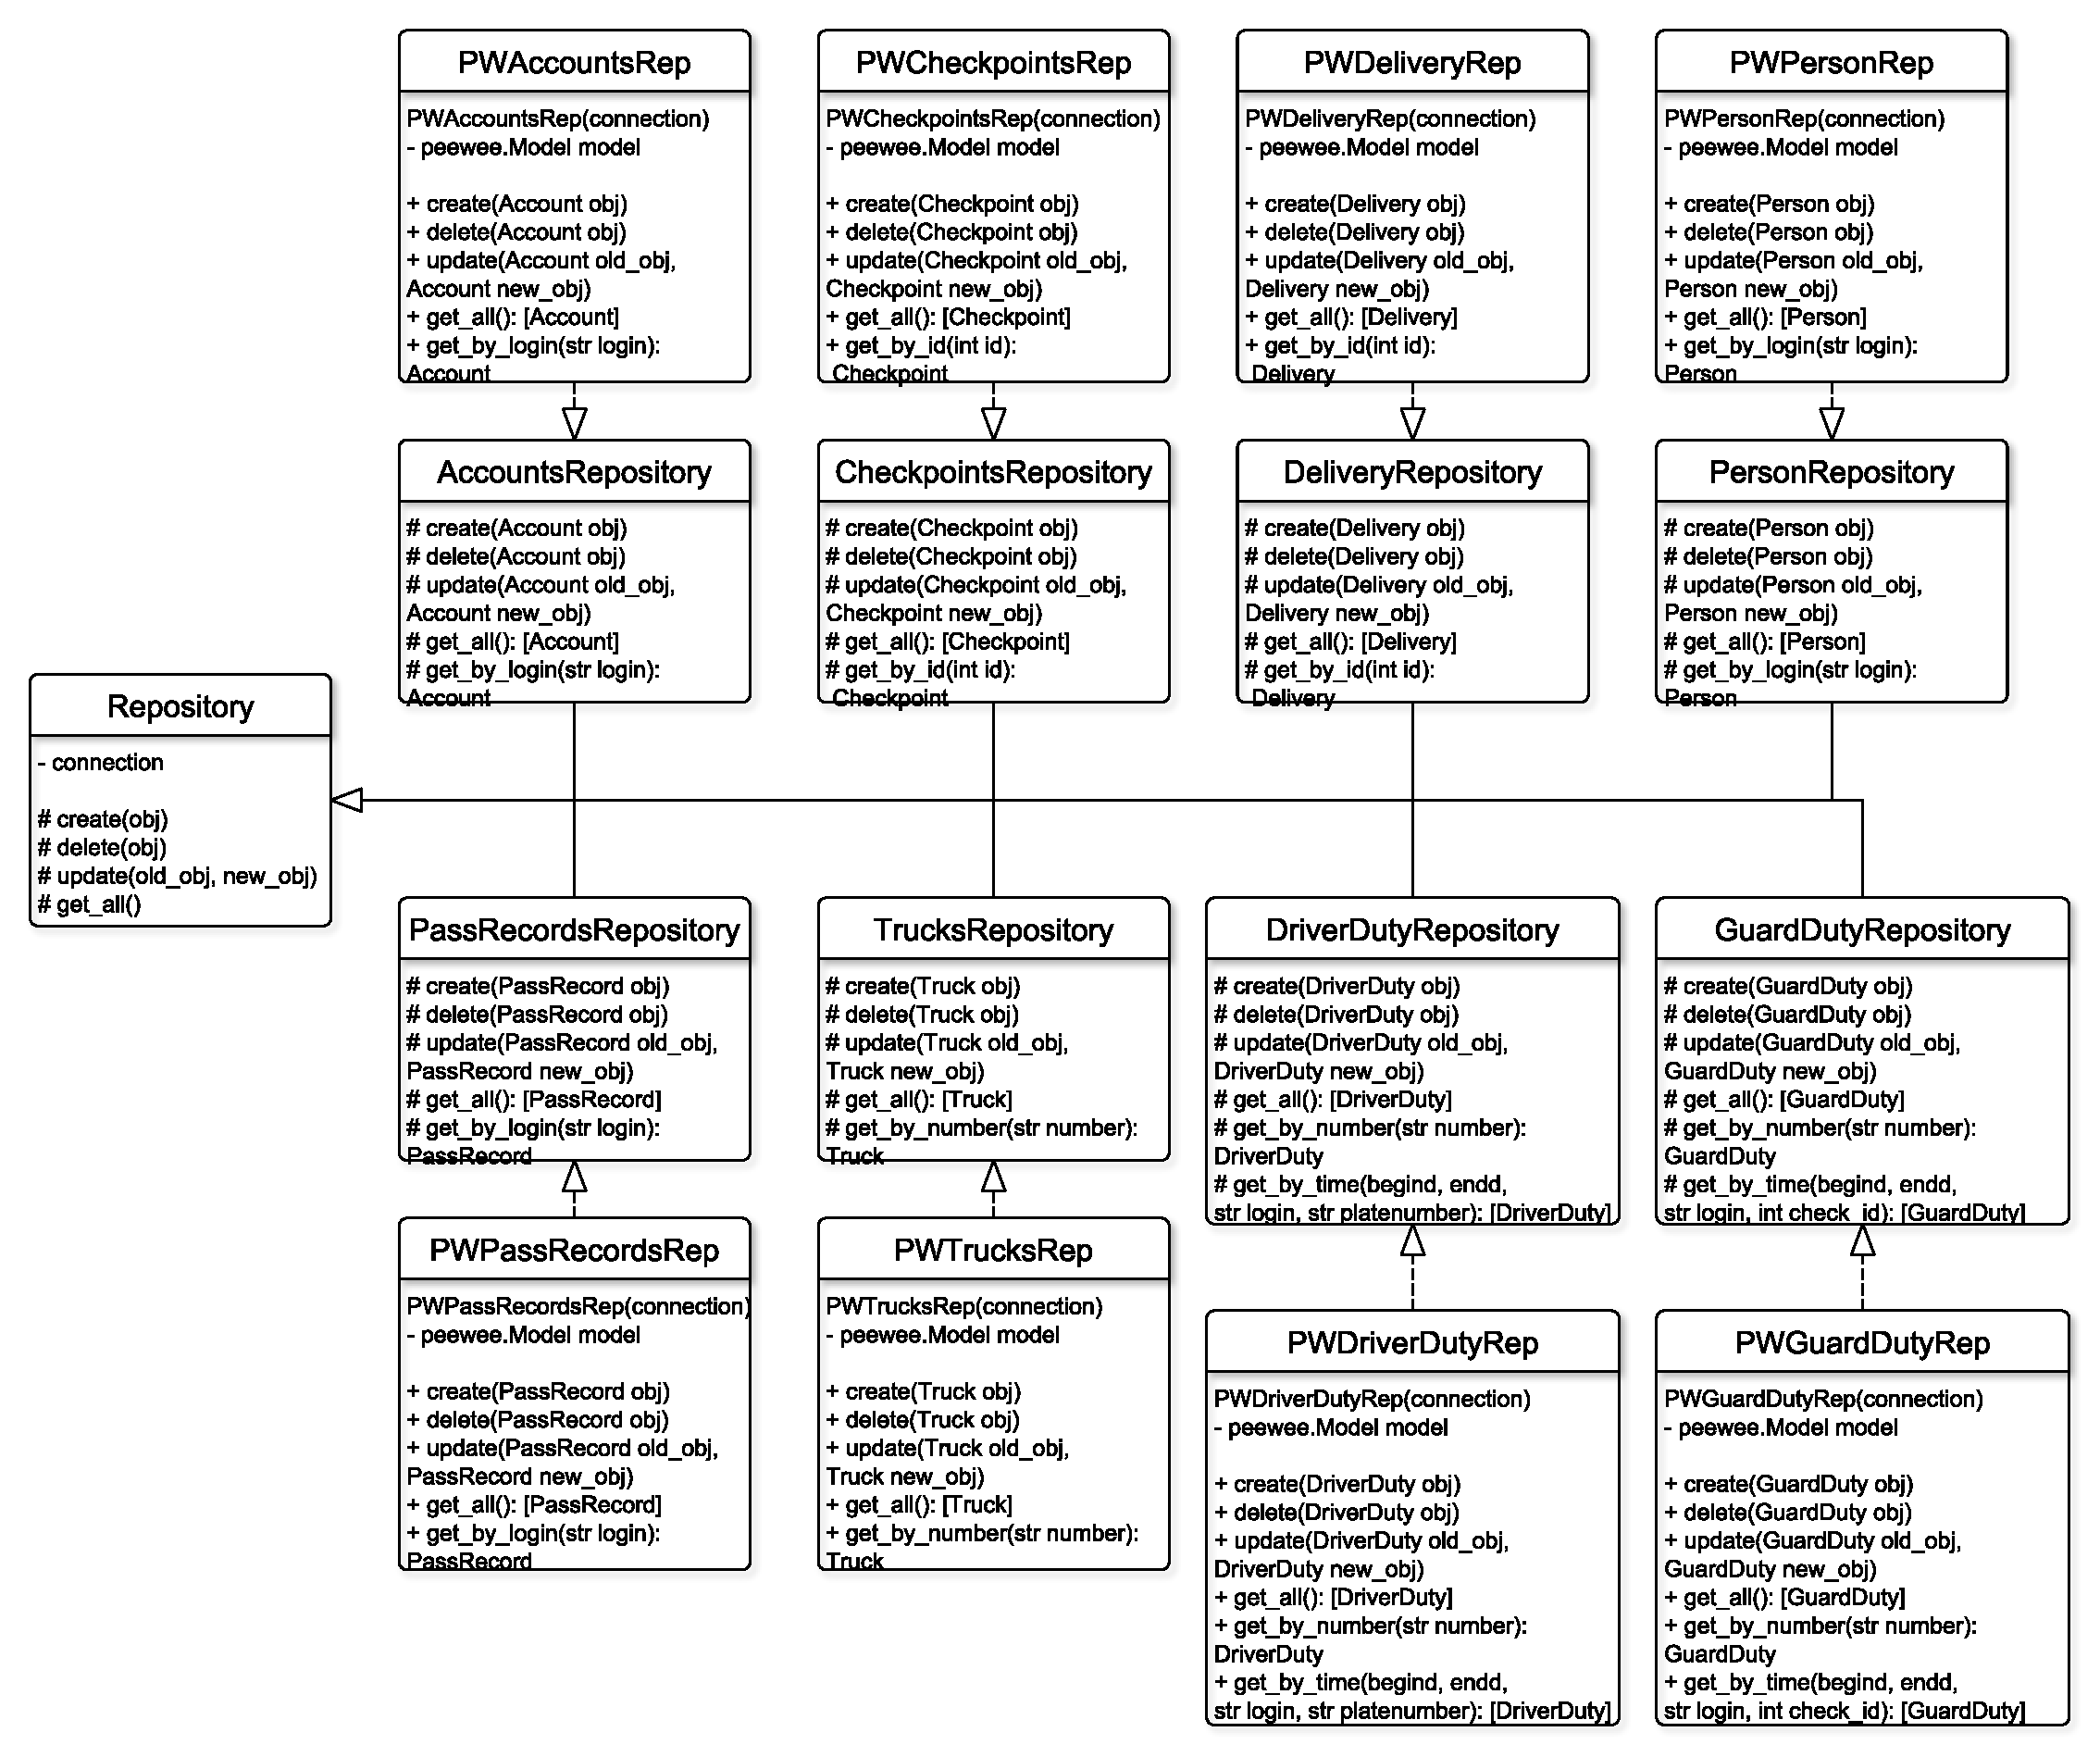
\includegraphics[height=14cm, width = 14cm]{uml/repsoitory.pdf}}
		{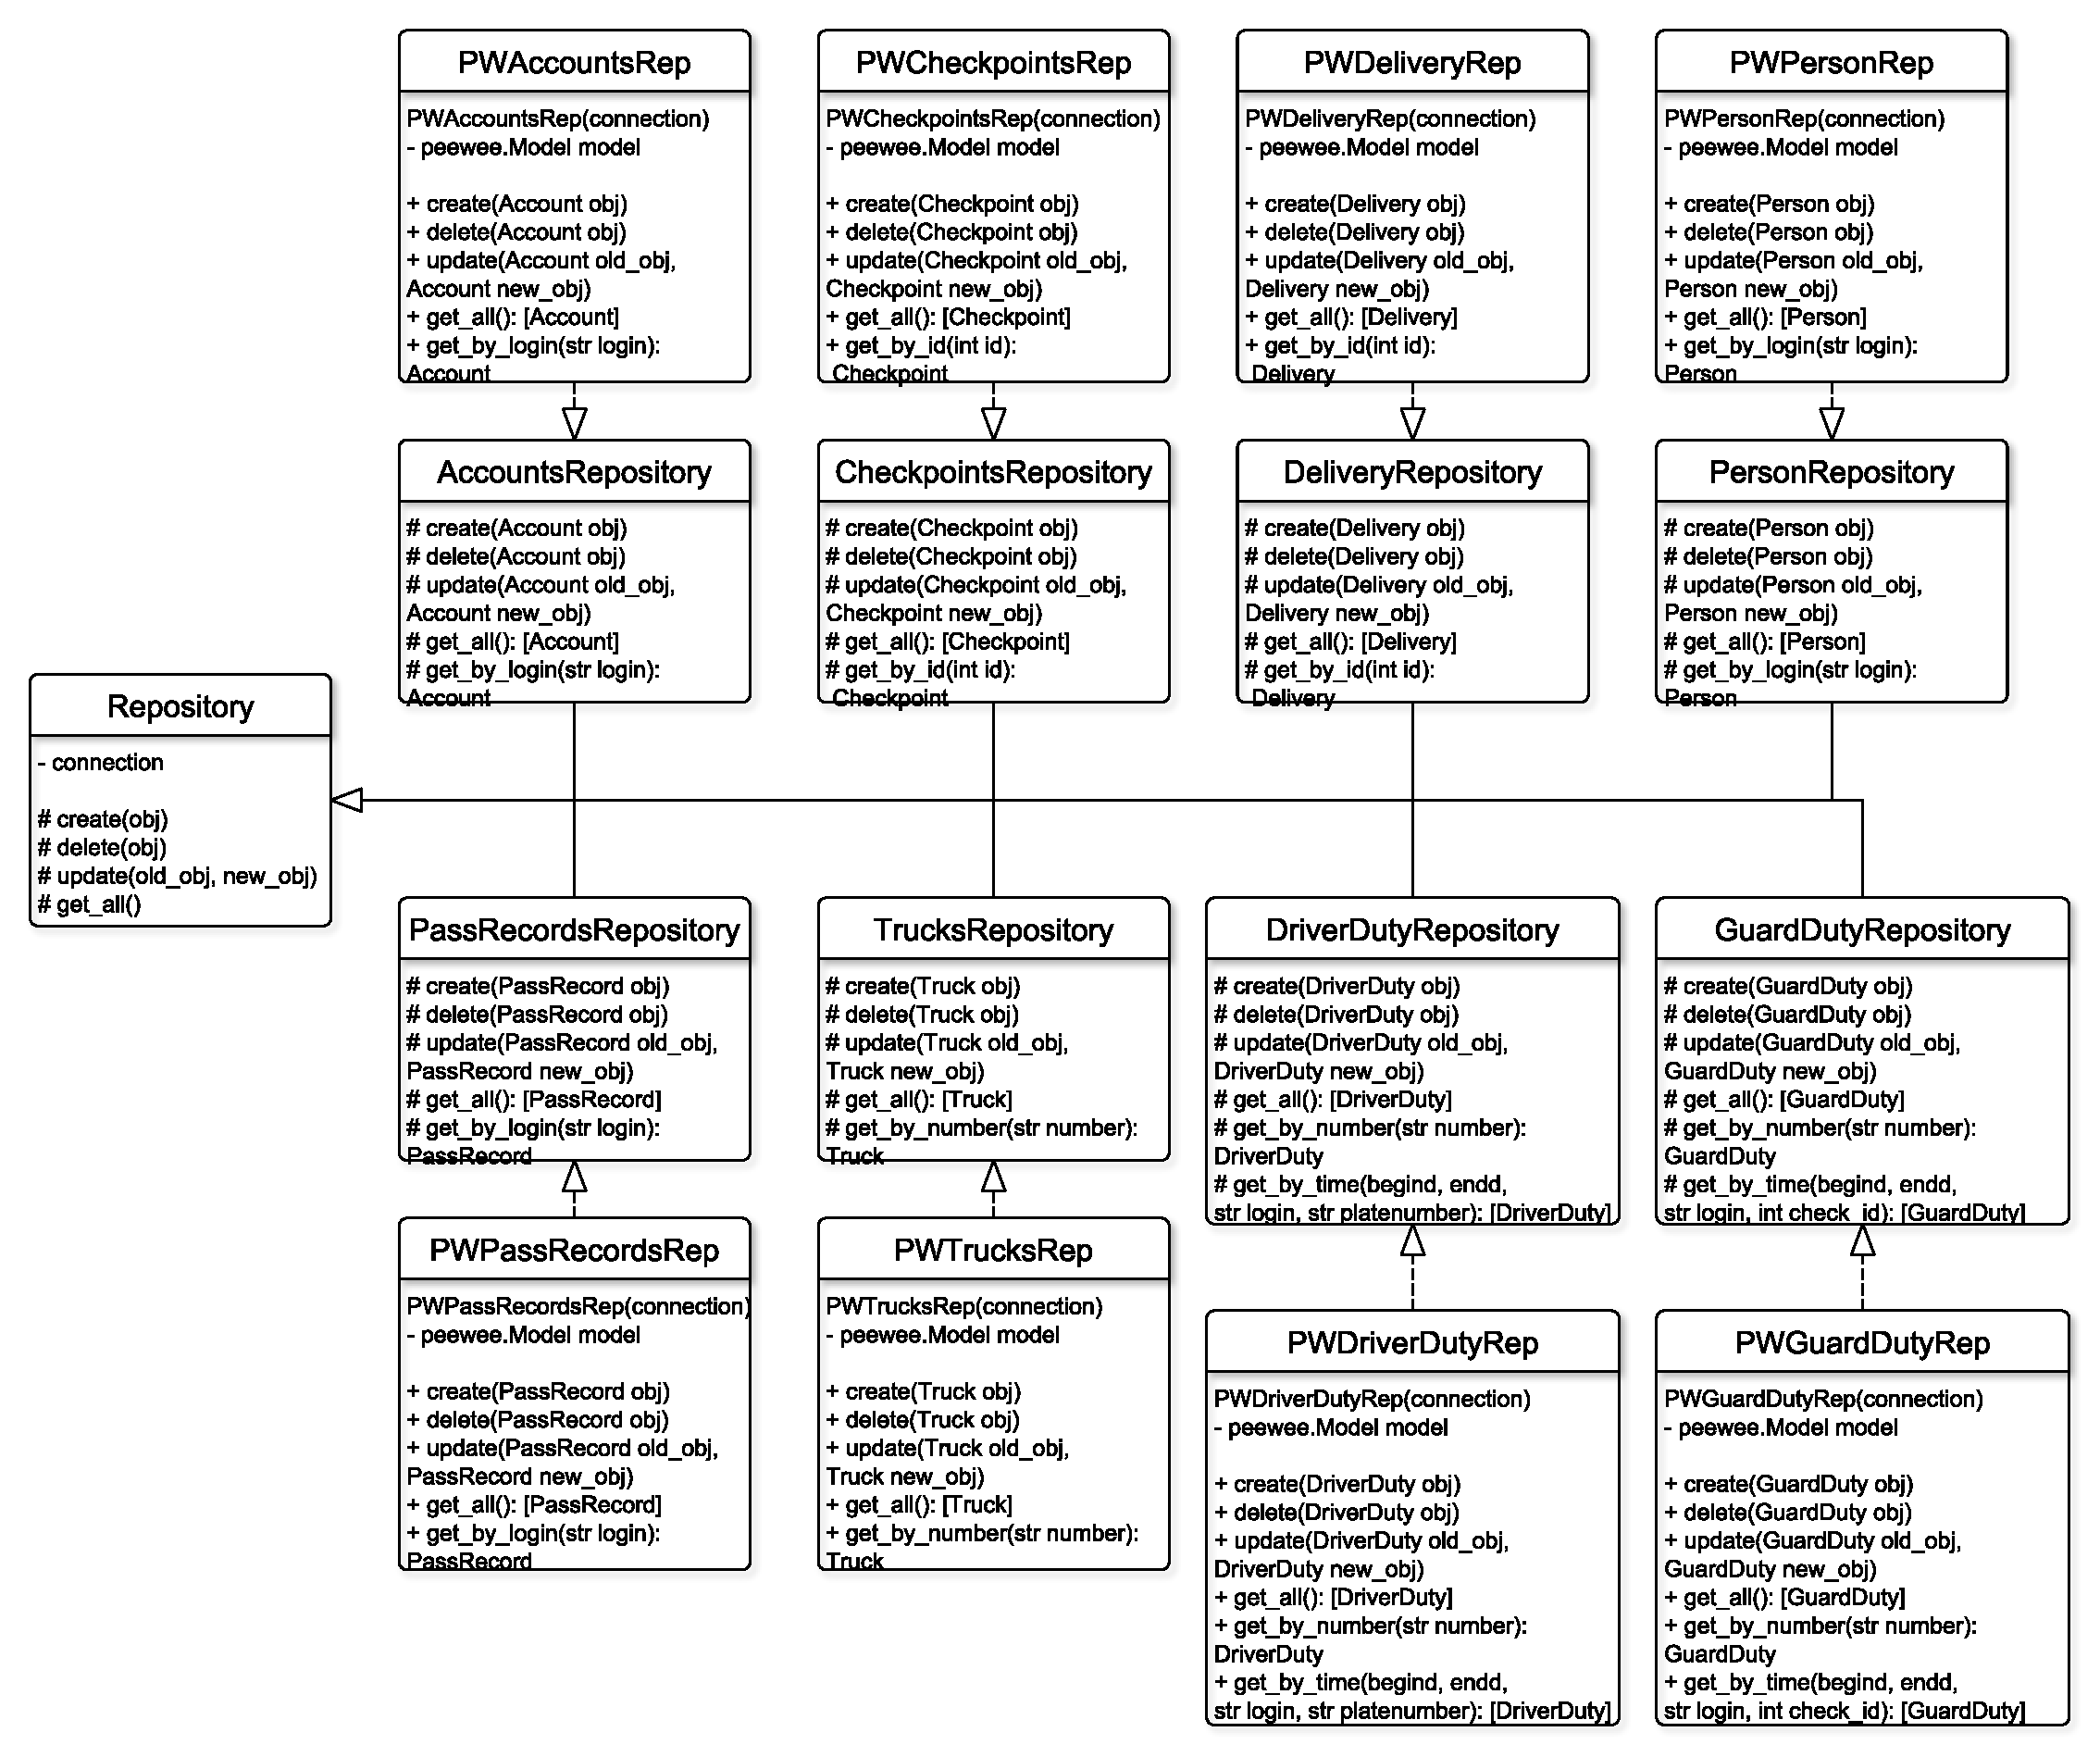
\includegraphics[scale=0.4, angle=0]{uml/repsoitory.pdf}}
		\caption{UML-диаграмма компонента доступа к данным}
	\end{center}
\end{figure}

\newpage
\subsection{Компонент бизнес-логики}
В соответствии с подходом MVC был создан компонент бизнес-логики, выполняющий основную обработку данных, UML диаграмма которого представленна на рисунке \hyperref[model_pic]{3.2}  

\begin{figure}[h!] \label{model_pic}
	\begin{center}
		%		{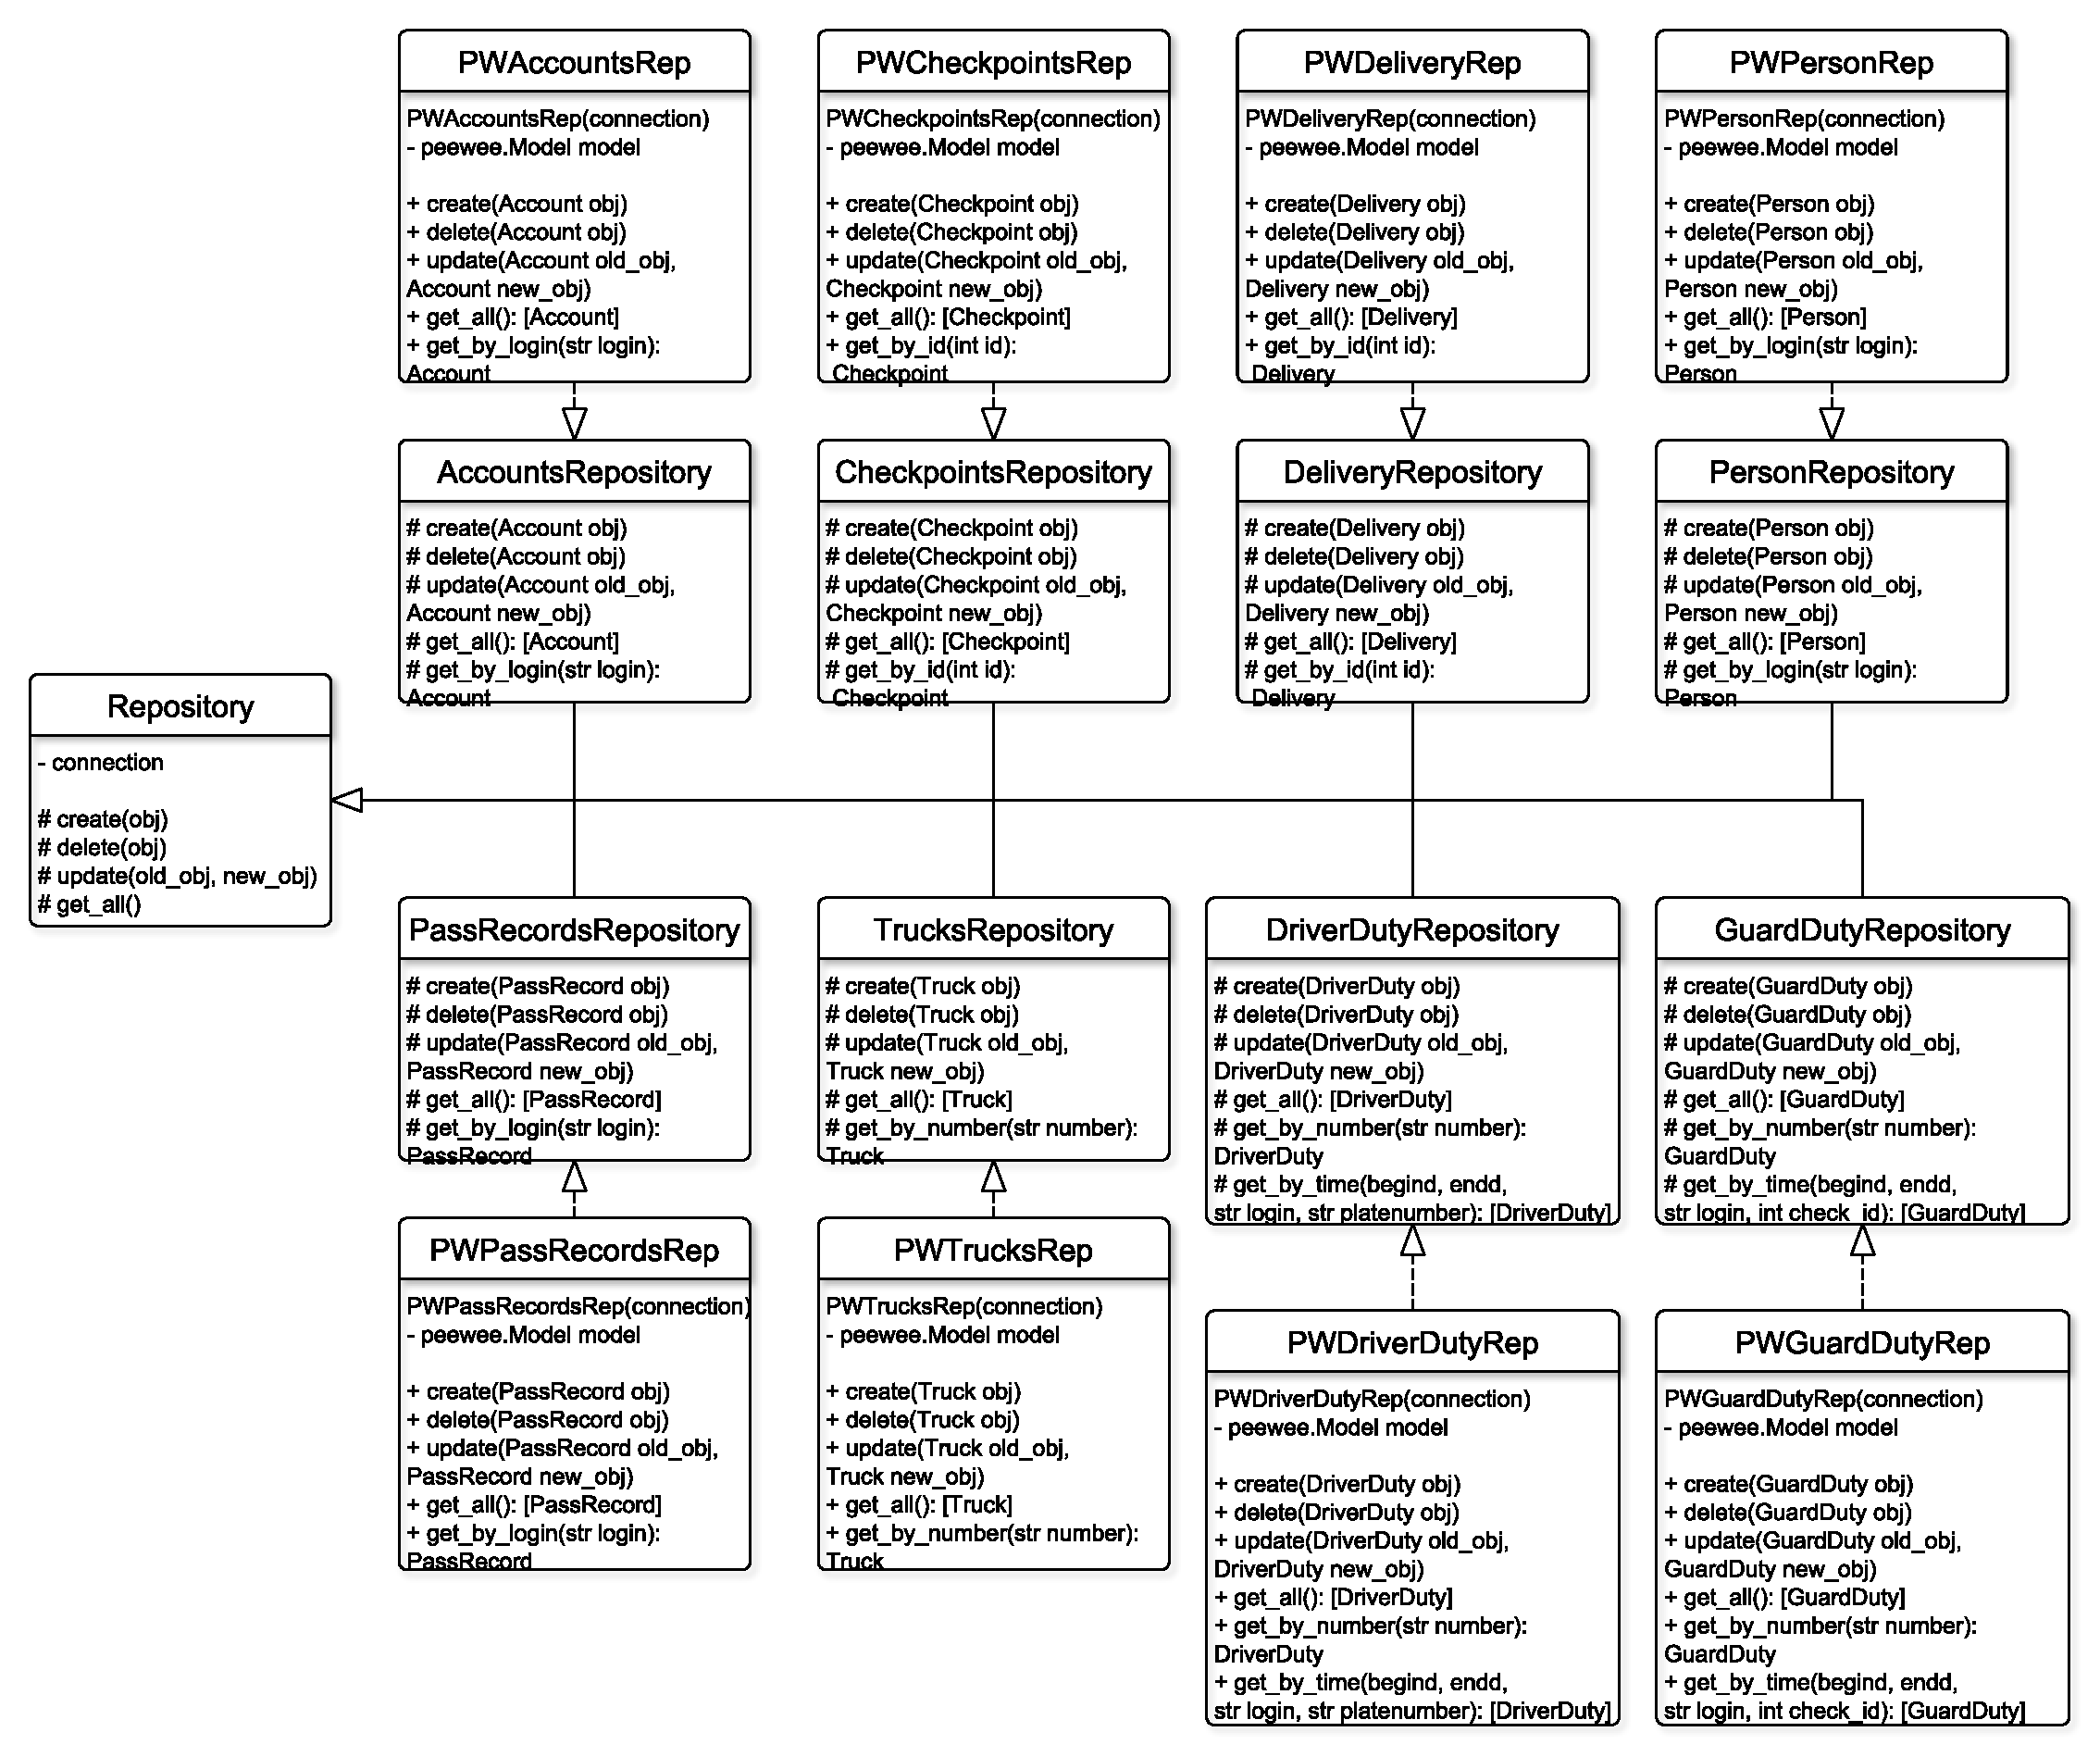
\includegraphics[height=14cm, width = 14cm]{uml/repsoitory.pdf}}
		{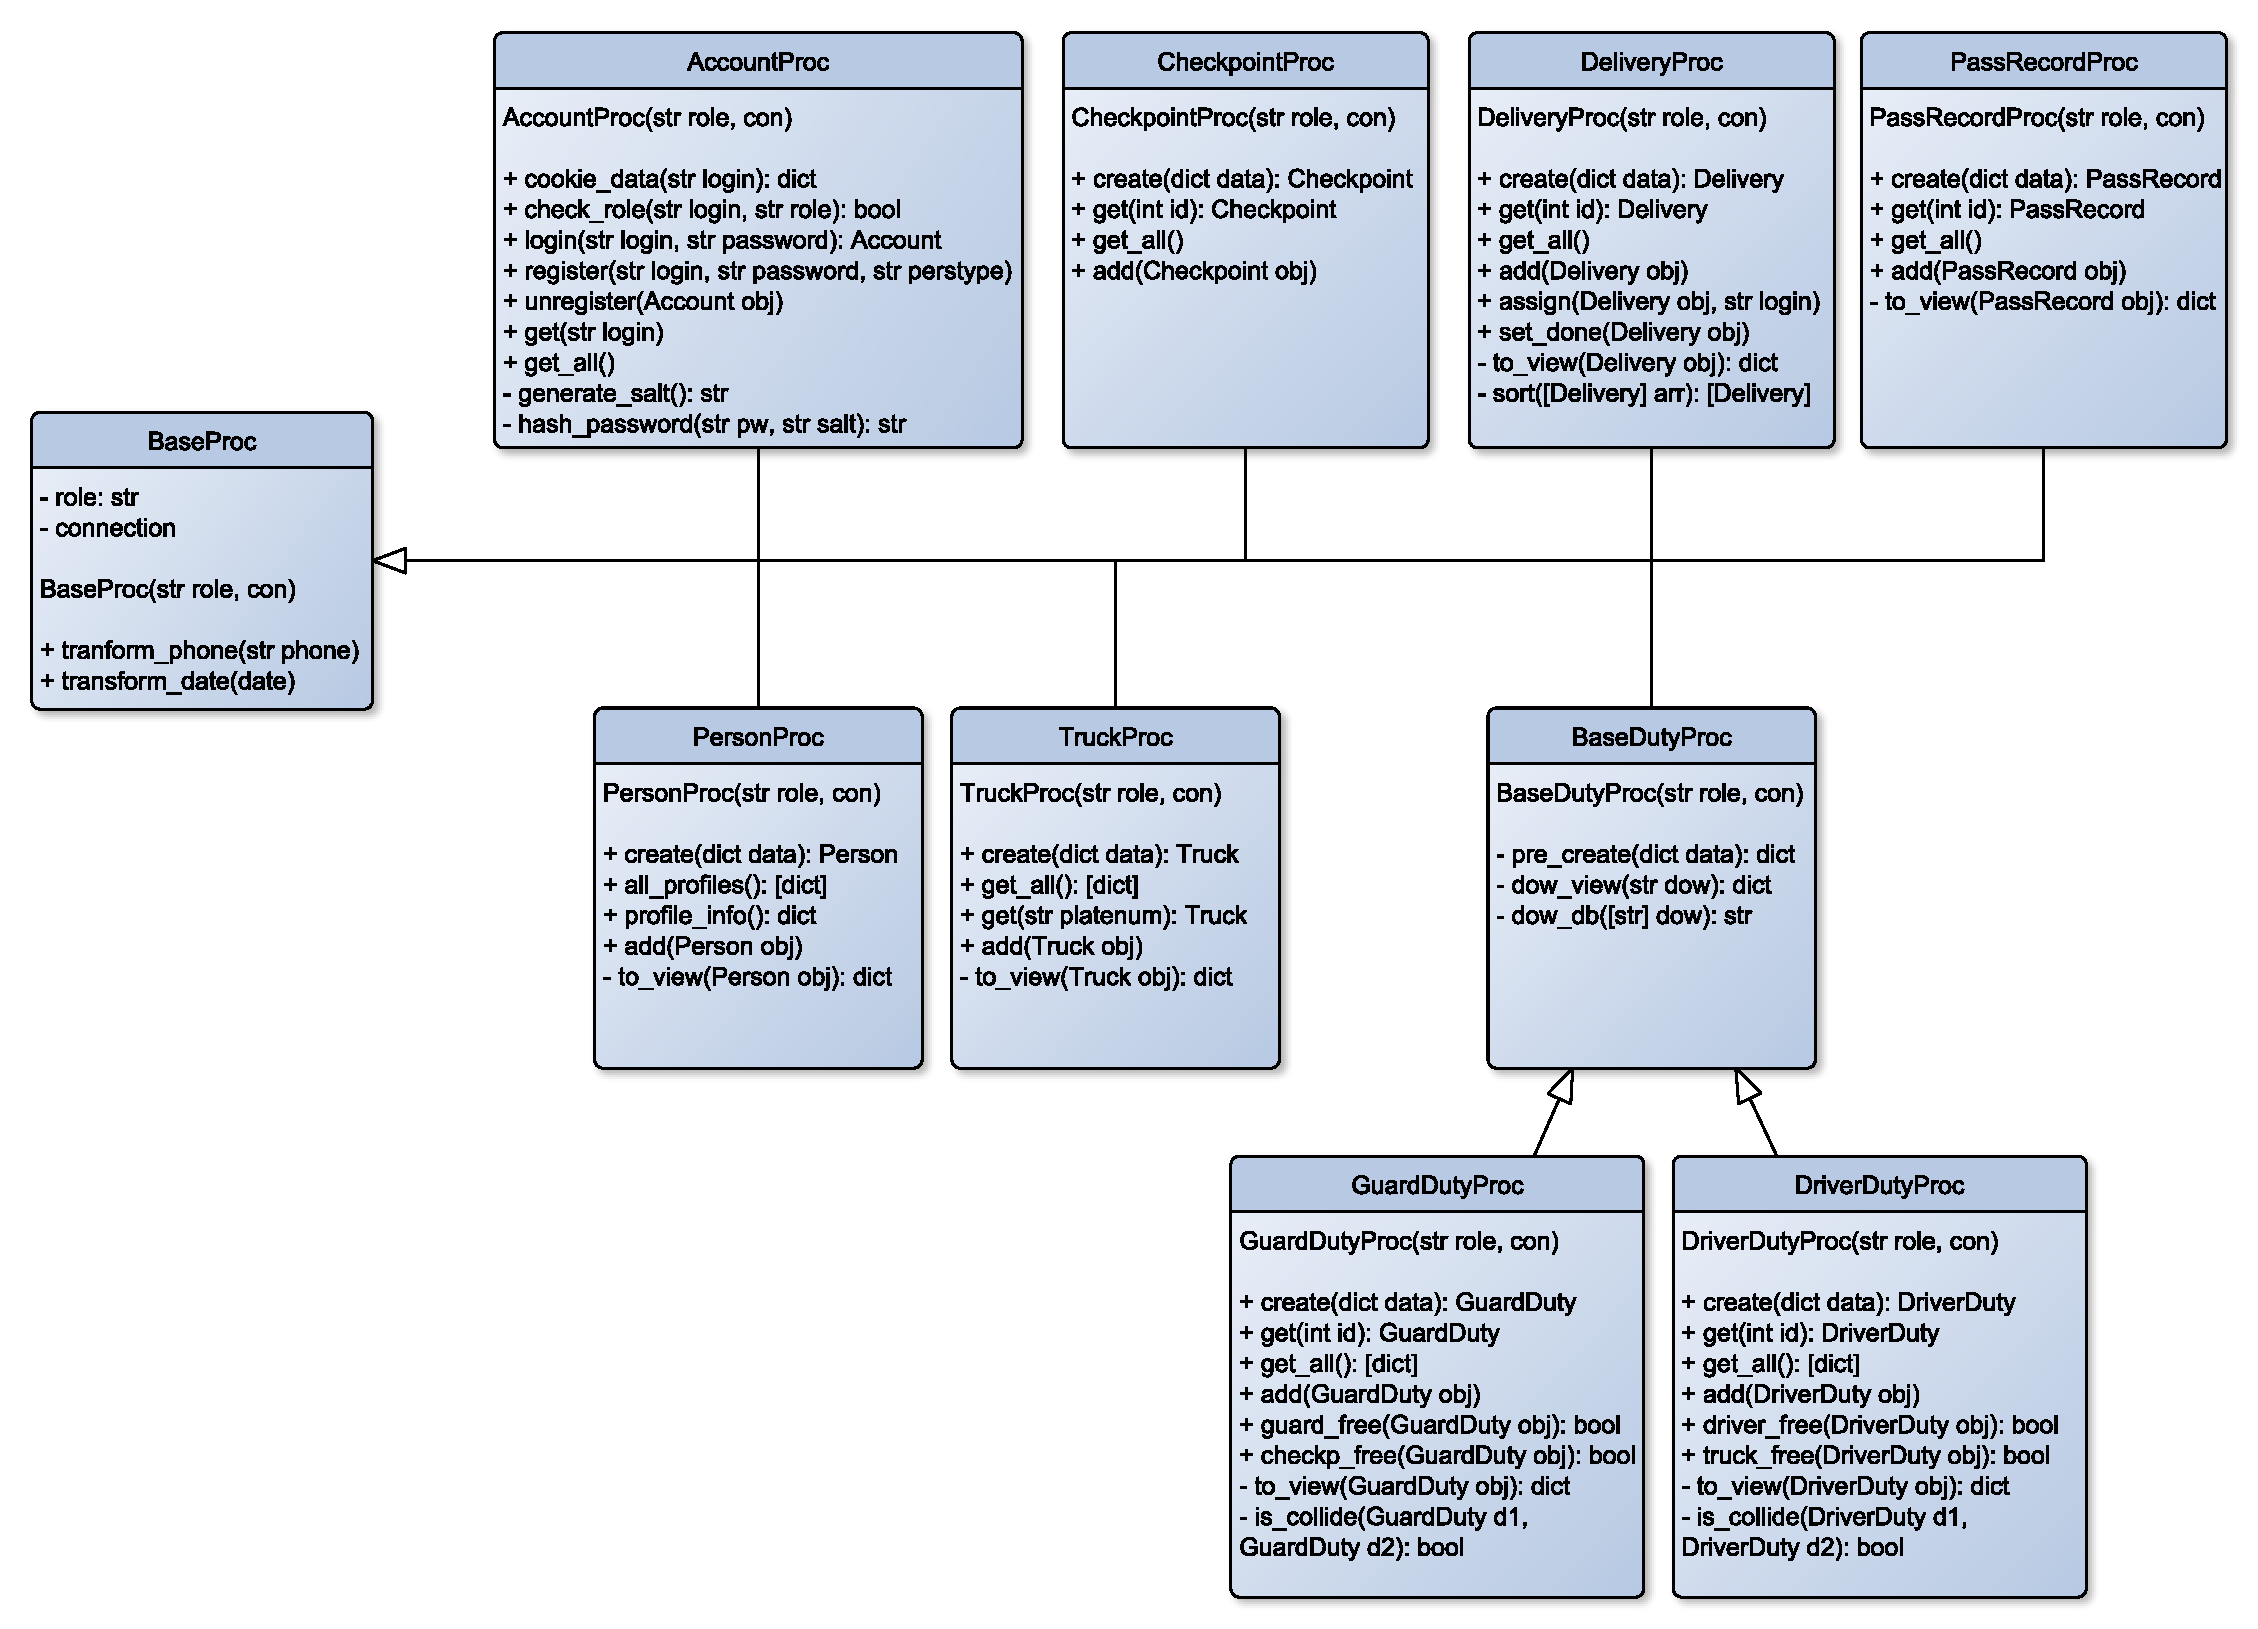
\includegraphics[scale=0.5, angle=0]{uml/business_models.pdf}}
		\caption{UML-диаграмма компонента бизнес-логики}
	\end{center}
\end{figure}

\newpage
\subsection{Компонент представления}
Также создан компонент представления, выполняющий отображение web-страниц в ответ на запросы пользователя, UML диаграмма которого представленна на рисунке \hyperref[view_pic]{3.3}. Помимо этого был реализован технический компонент представления, отображающий информацию в символьном виде, для возможности тестирования компонента бизнес-логики.

\begin{figure}[h!] \label{view_pic}
	\begin{center}
		%		{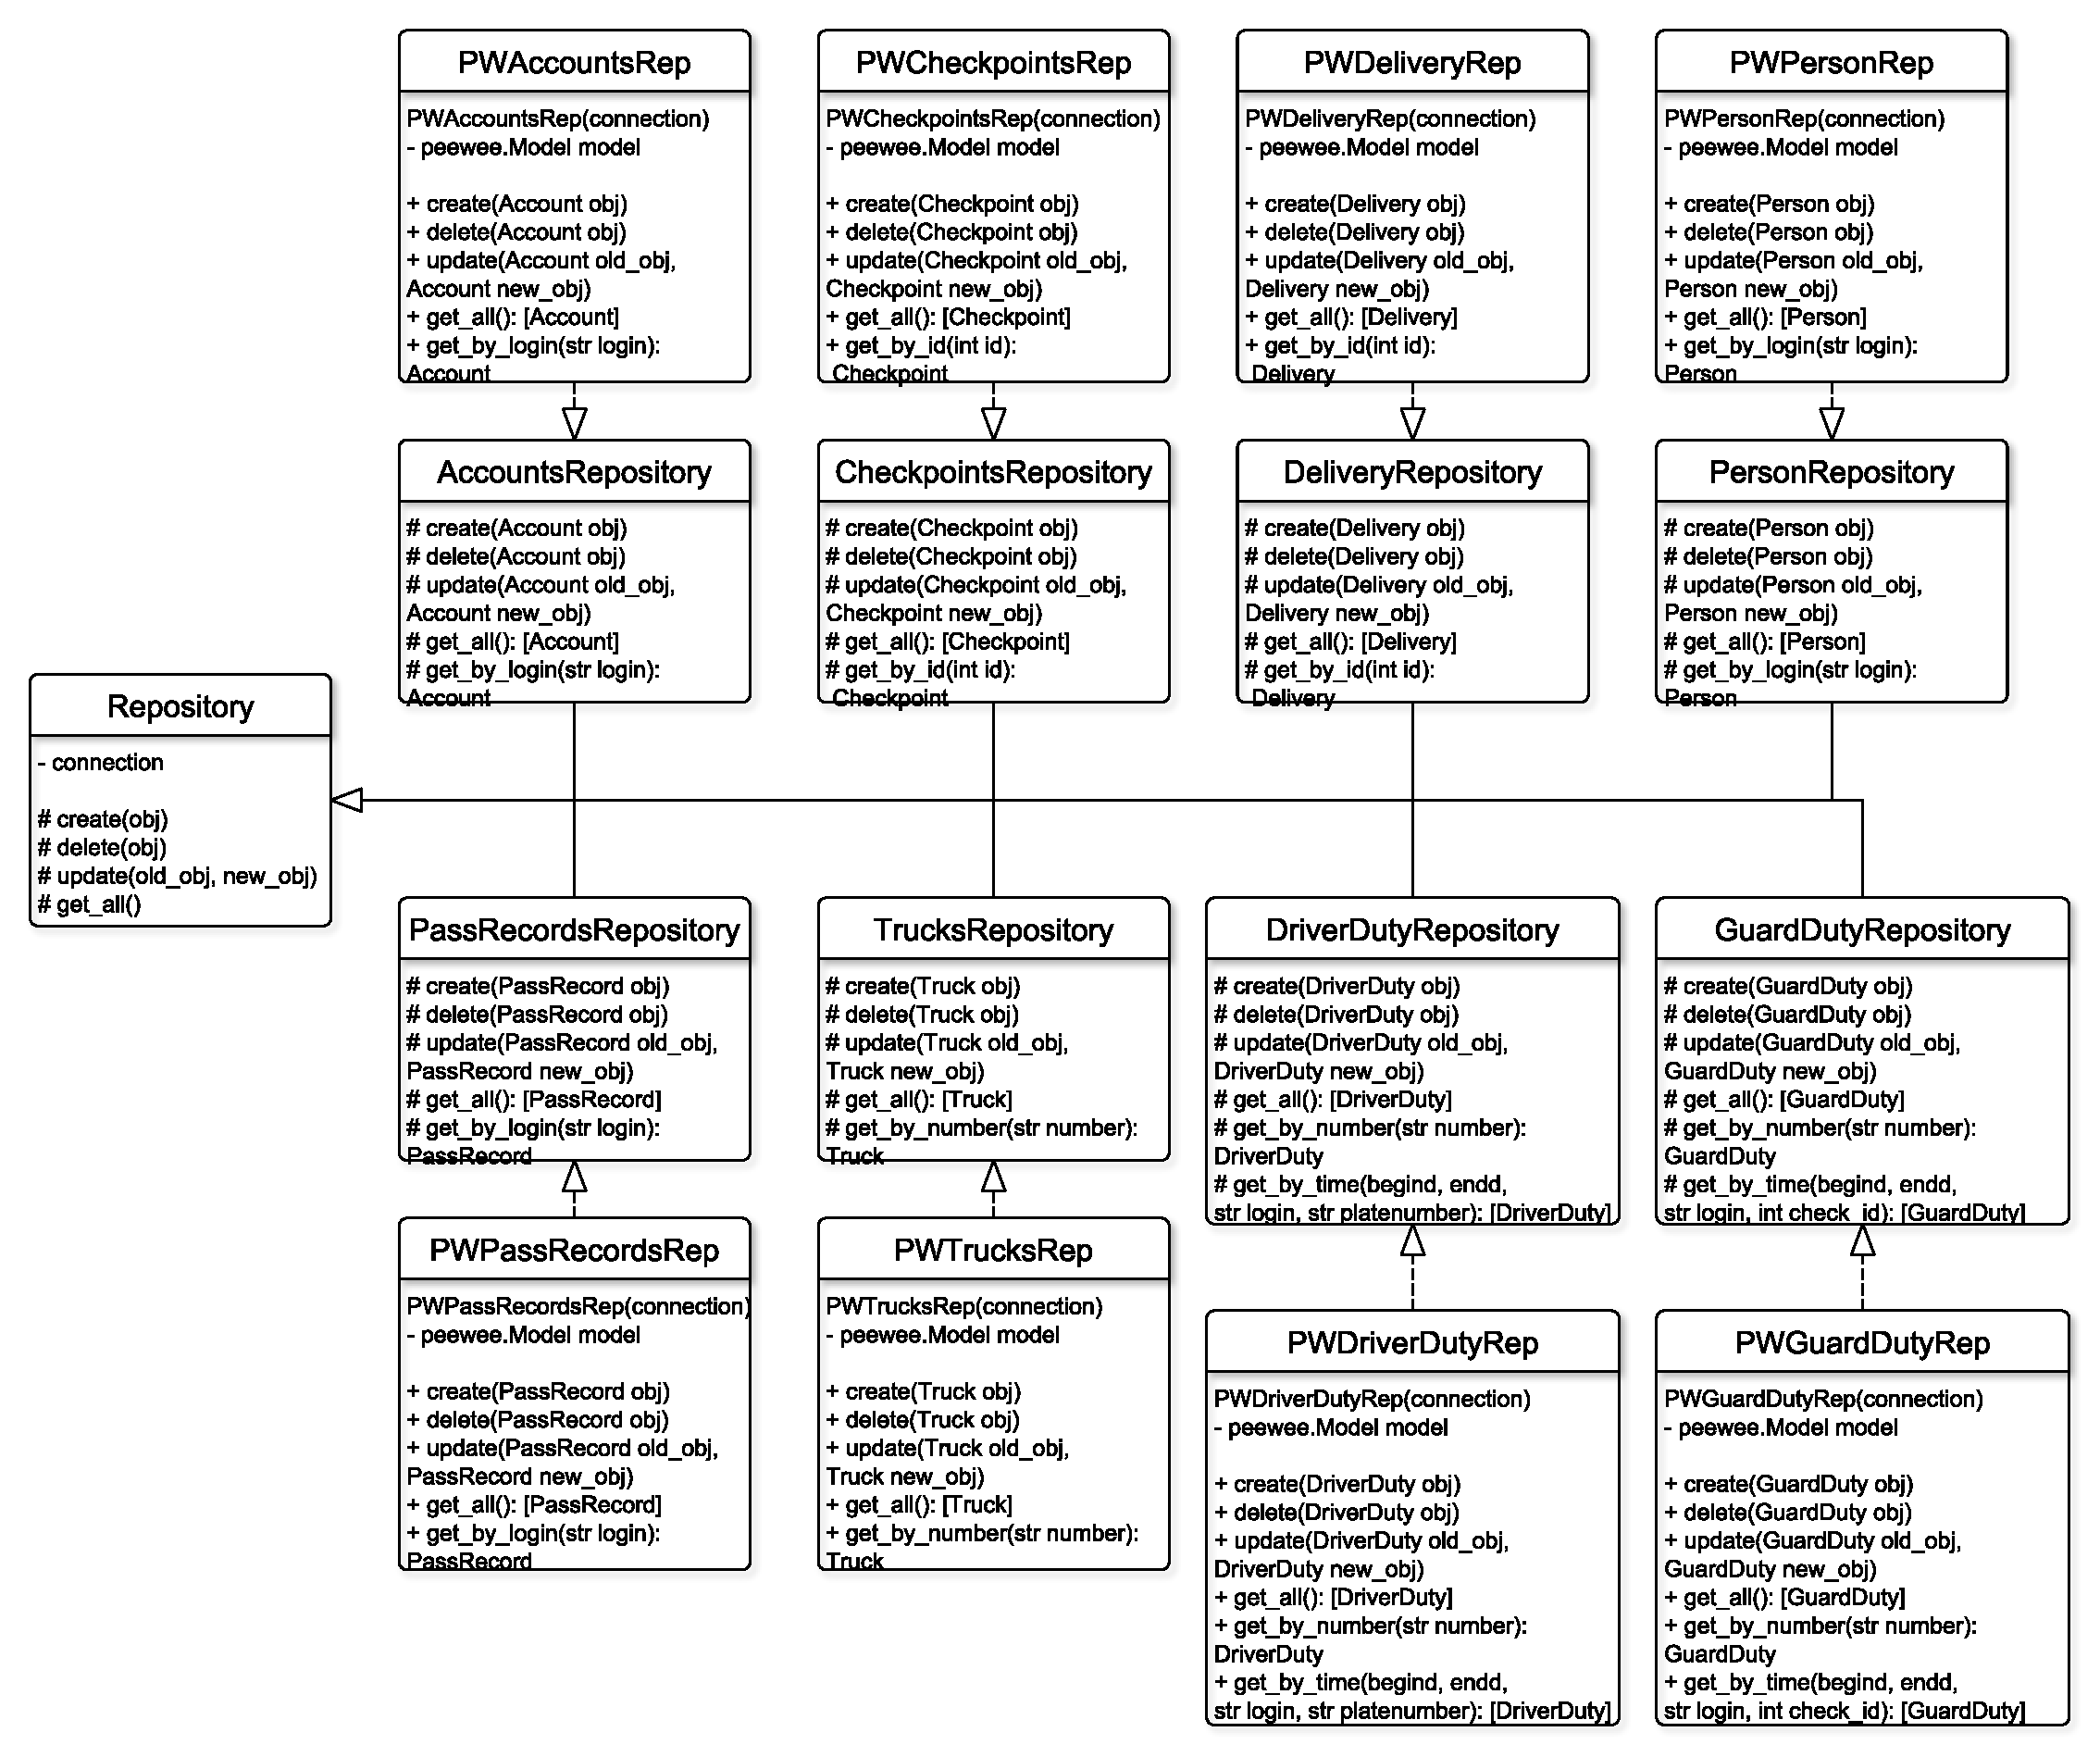
\includegraphics[height=14cm, width = 14cm]{uml/repsoitory.pdf}}
		{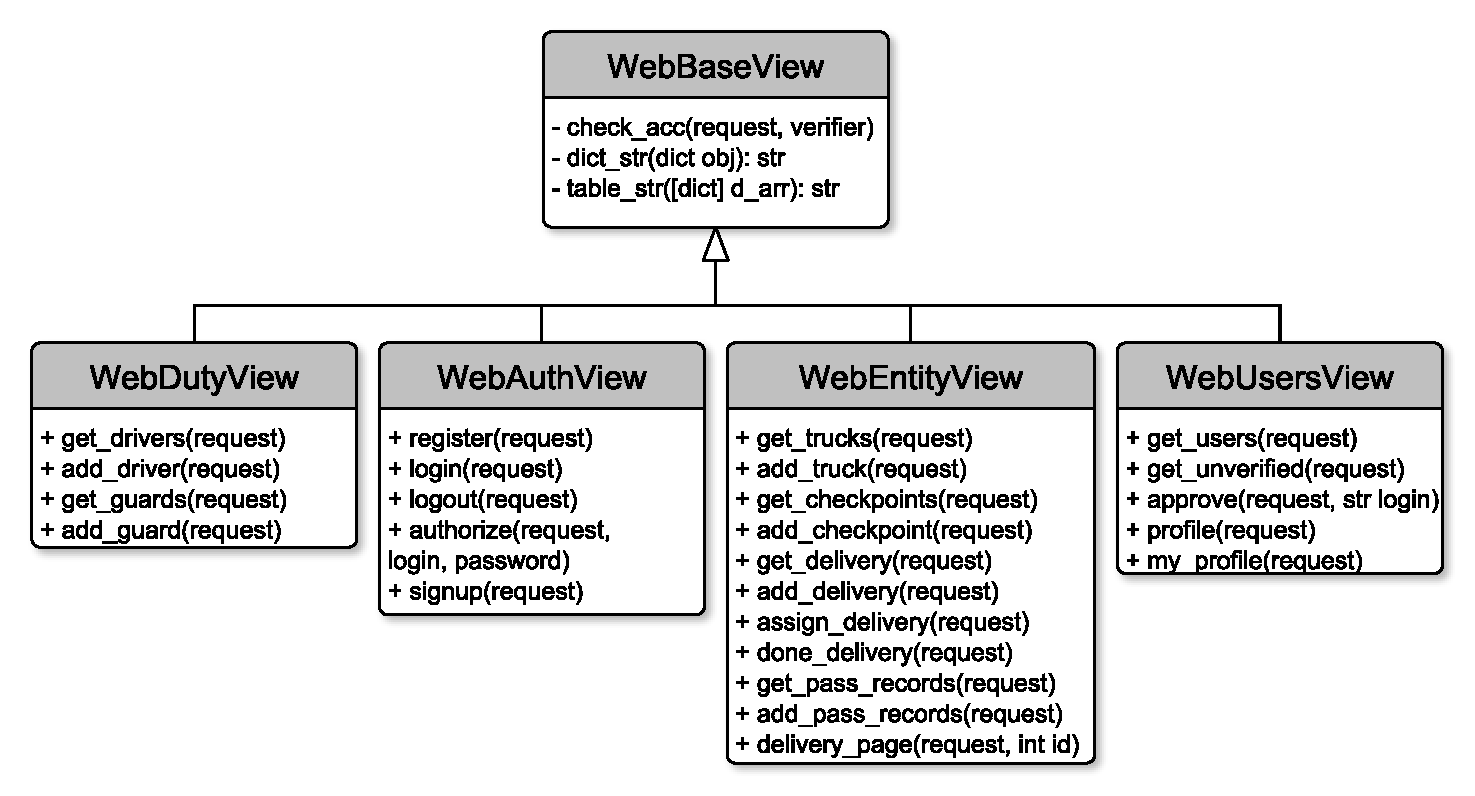
\includegraphics[scale=0.5, angle=0]{uml/webGUI.pdf}}
		\caption{UML-диаграмма компонента web-представления}
	\end{center}
\end{figure}

\newpage
\subsection{Диаграмма приложения}
Все перечисленные компоненты можно объединить в одну UML-диаграмму всего приложения на рисунке \hyperref[alluml_pic]{3.4}

\begin{figure}[h!] \label{alluml_pic}
	\begin{center}
		%		{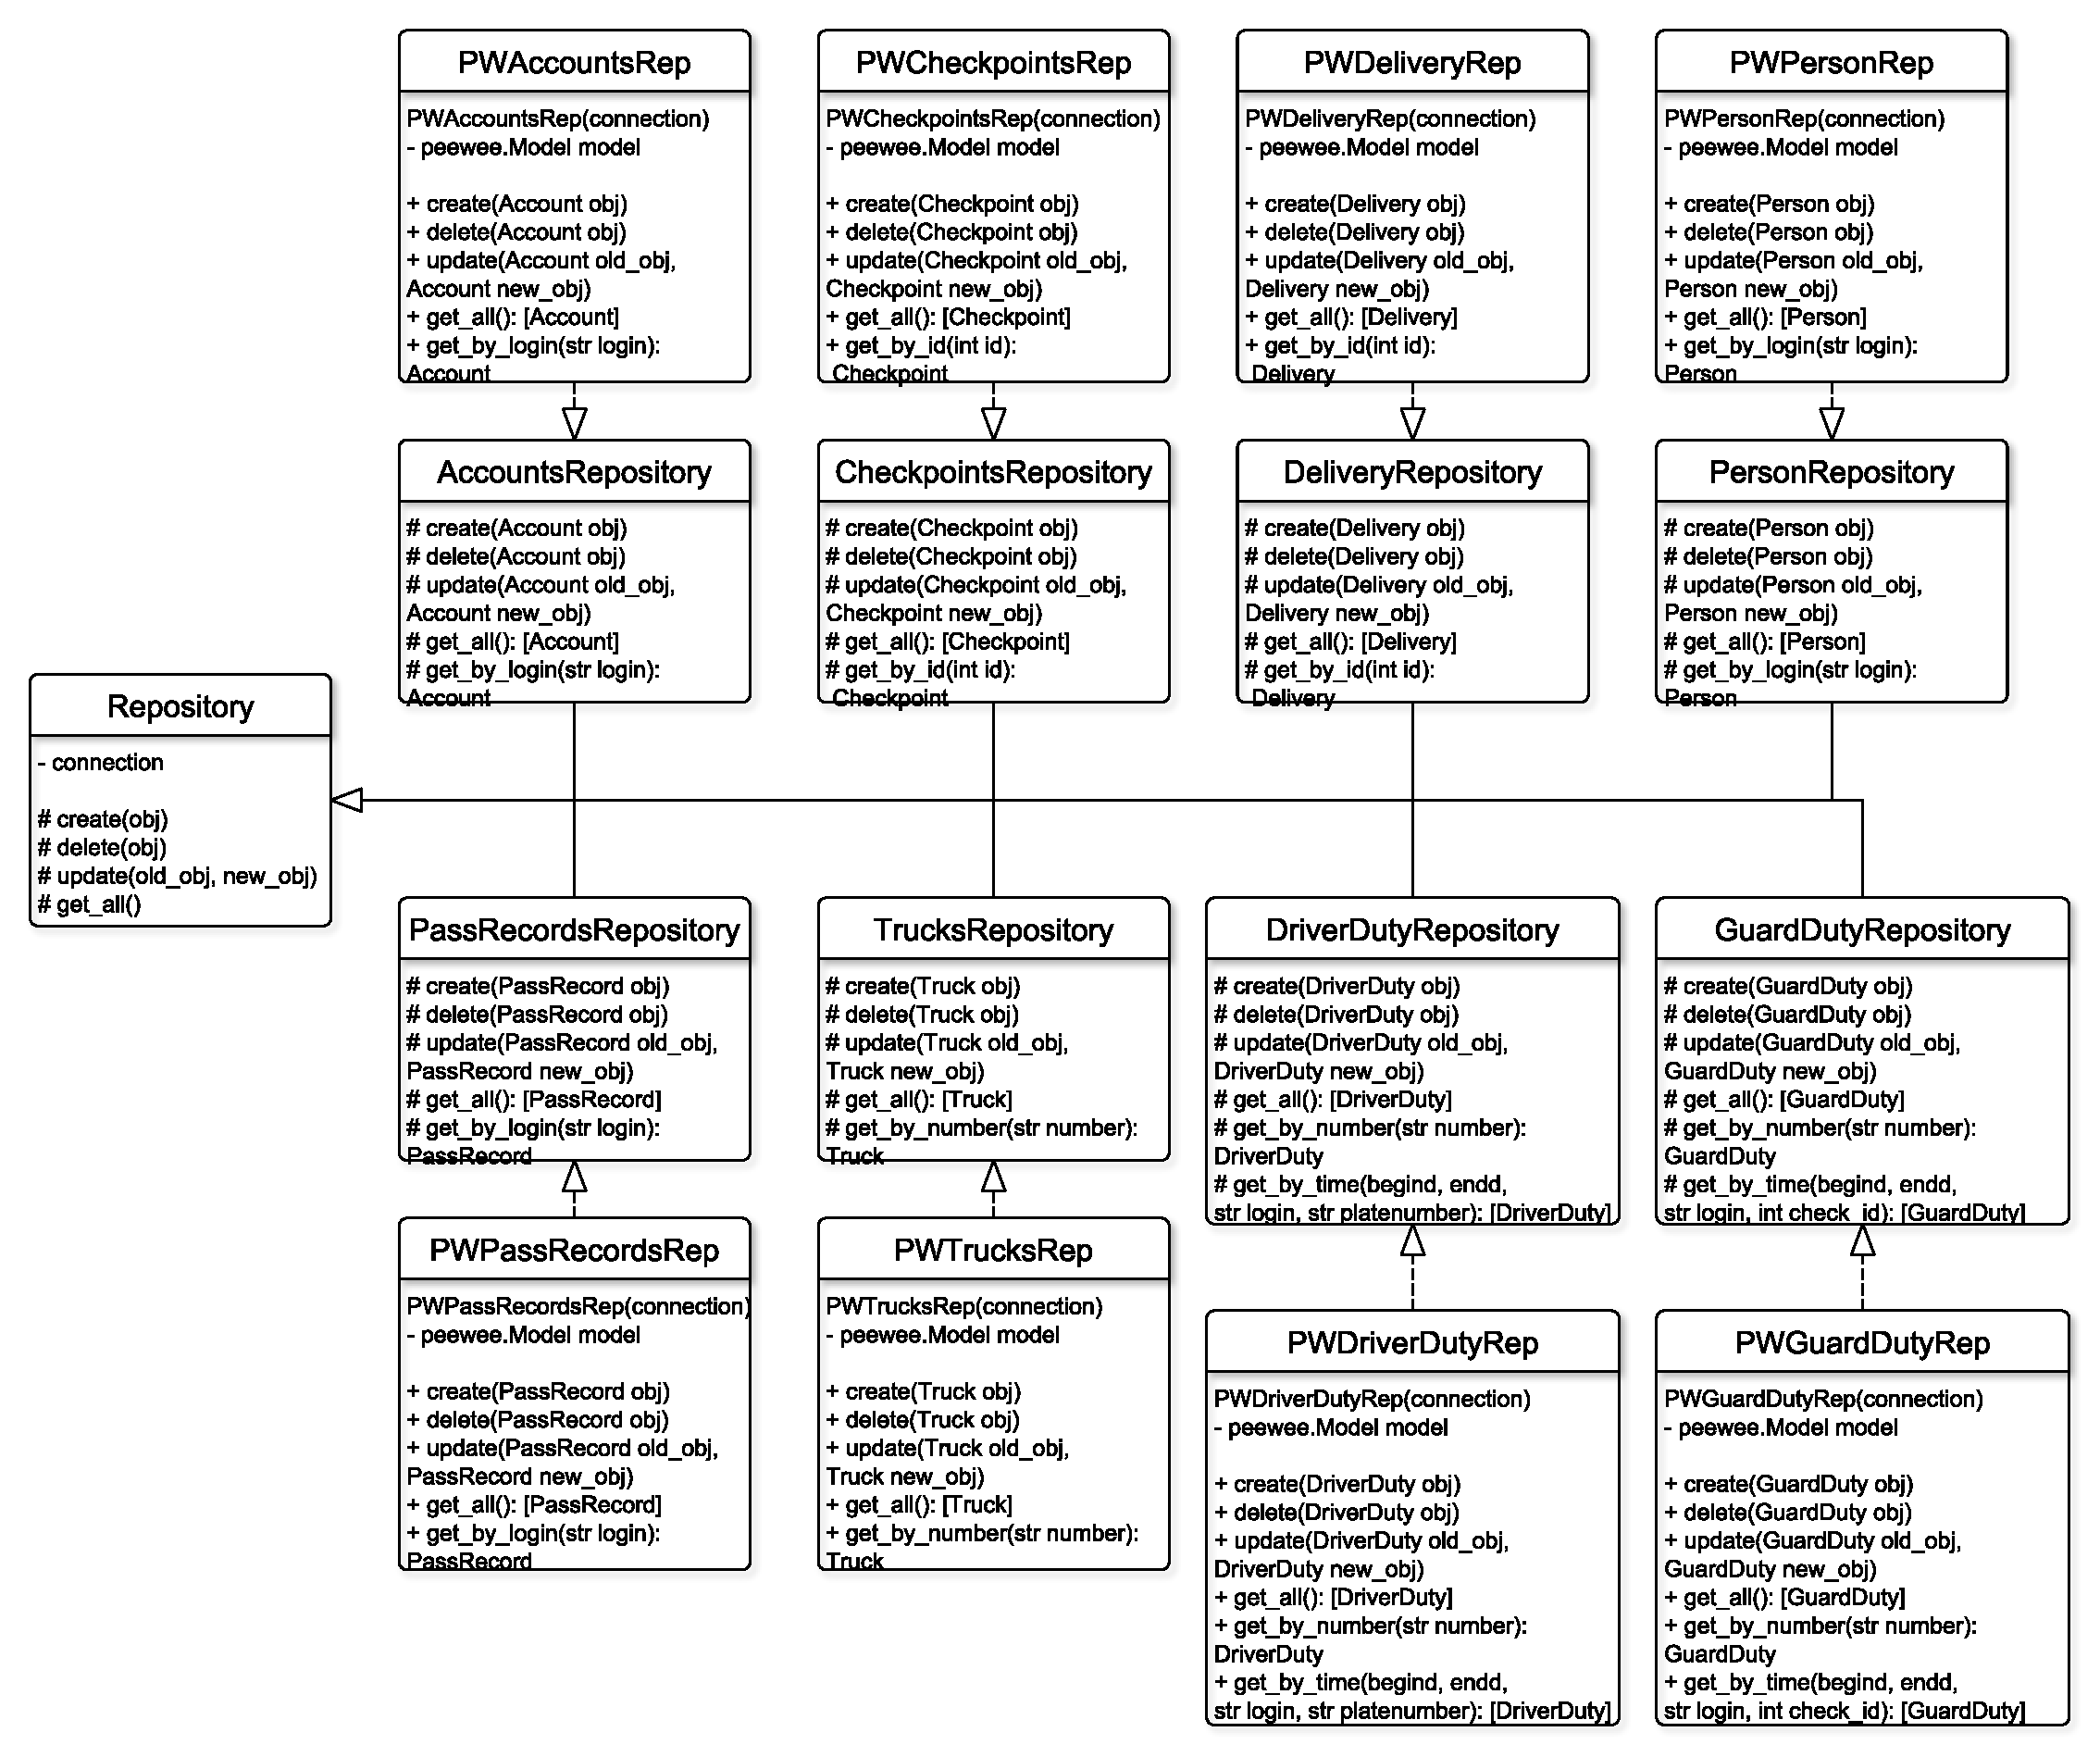
\includegraphics[height=14cm, width = 14cm]{uml/repsoitory.pdf}}
		{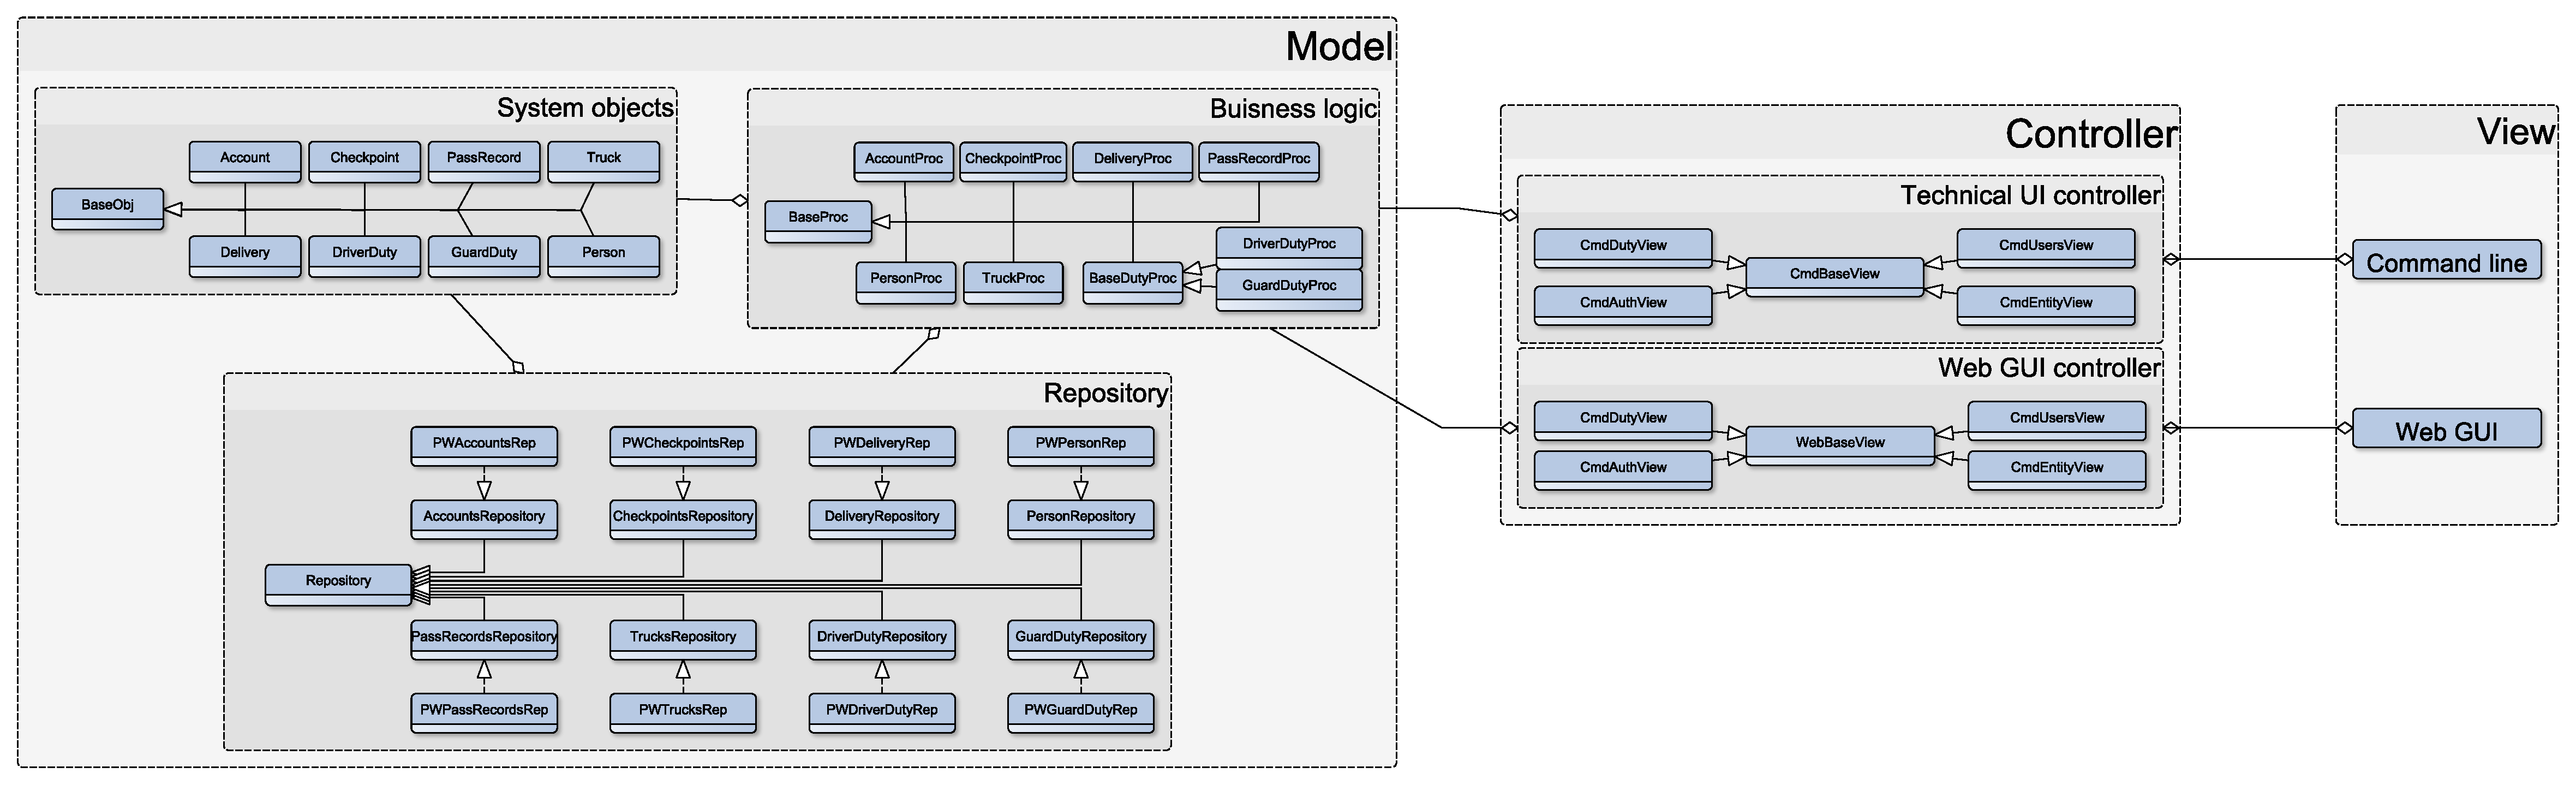
\includegraphics[scale=0.36, angle=-90]{uml/components.pdf}}
		\caption{UML-диаграмма компонента web-представления}
	\end{center}
\end{figure}


\section{Интерфейс приложения}
Для авторизованного пользователя в заголовке каждой страницы содержится панель навигации, предоставляющая возможность перейти на все страницы, функционально соответствующие его роли. Данная панель изображена на примере администратора на рисунке \hyperref[navbar_sc]{3.5}. Некоторые пункты меню являются выпадающими, их можно открыть наведением мыши. Также в левом углу панели присутствует элемент информационного или ошибочного сообщения.

На рисунках \hyperref[navbar_sc]{3.5}-\hyperref[trucks_sc]{3.11} приведена демонстрация ключевых страниц для роли администратора. На рисунках \hyperref[pick_delivery_sc]{3.12}, \hyperref[driver_profile_sc]{3.13} и \hyperref[guard_duty_sc]{3.14}, \hyperref[guard_duty_sc]{3.15} приведены страницы, уникальные для ролей водителя и охранника соотвественно.

\begin{figure}[h!] \label{navbar_sc}
	\begin{center}
		%		{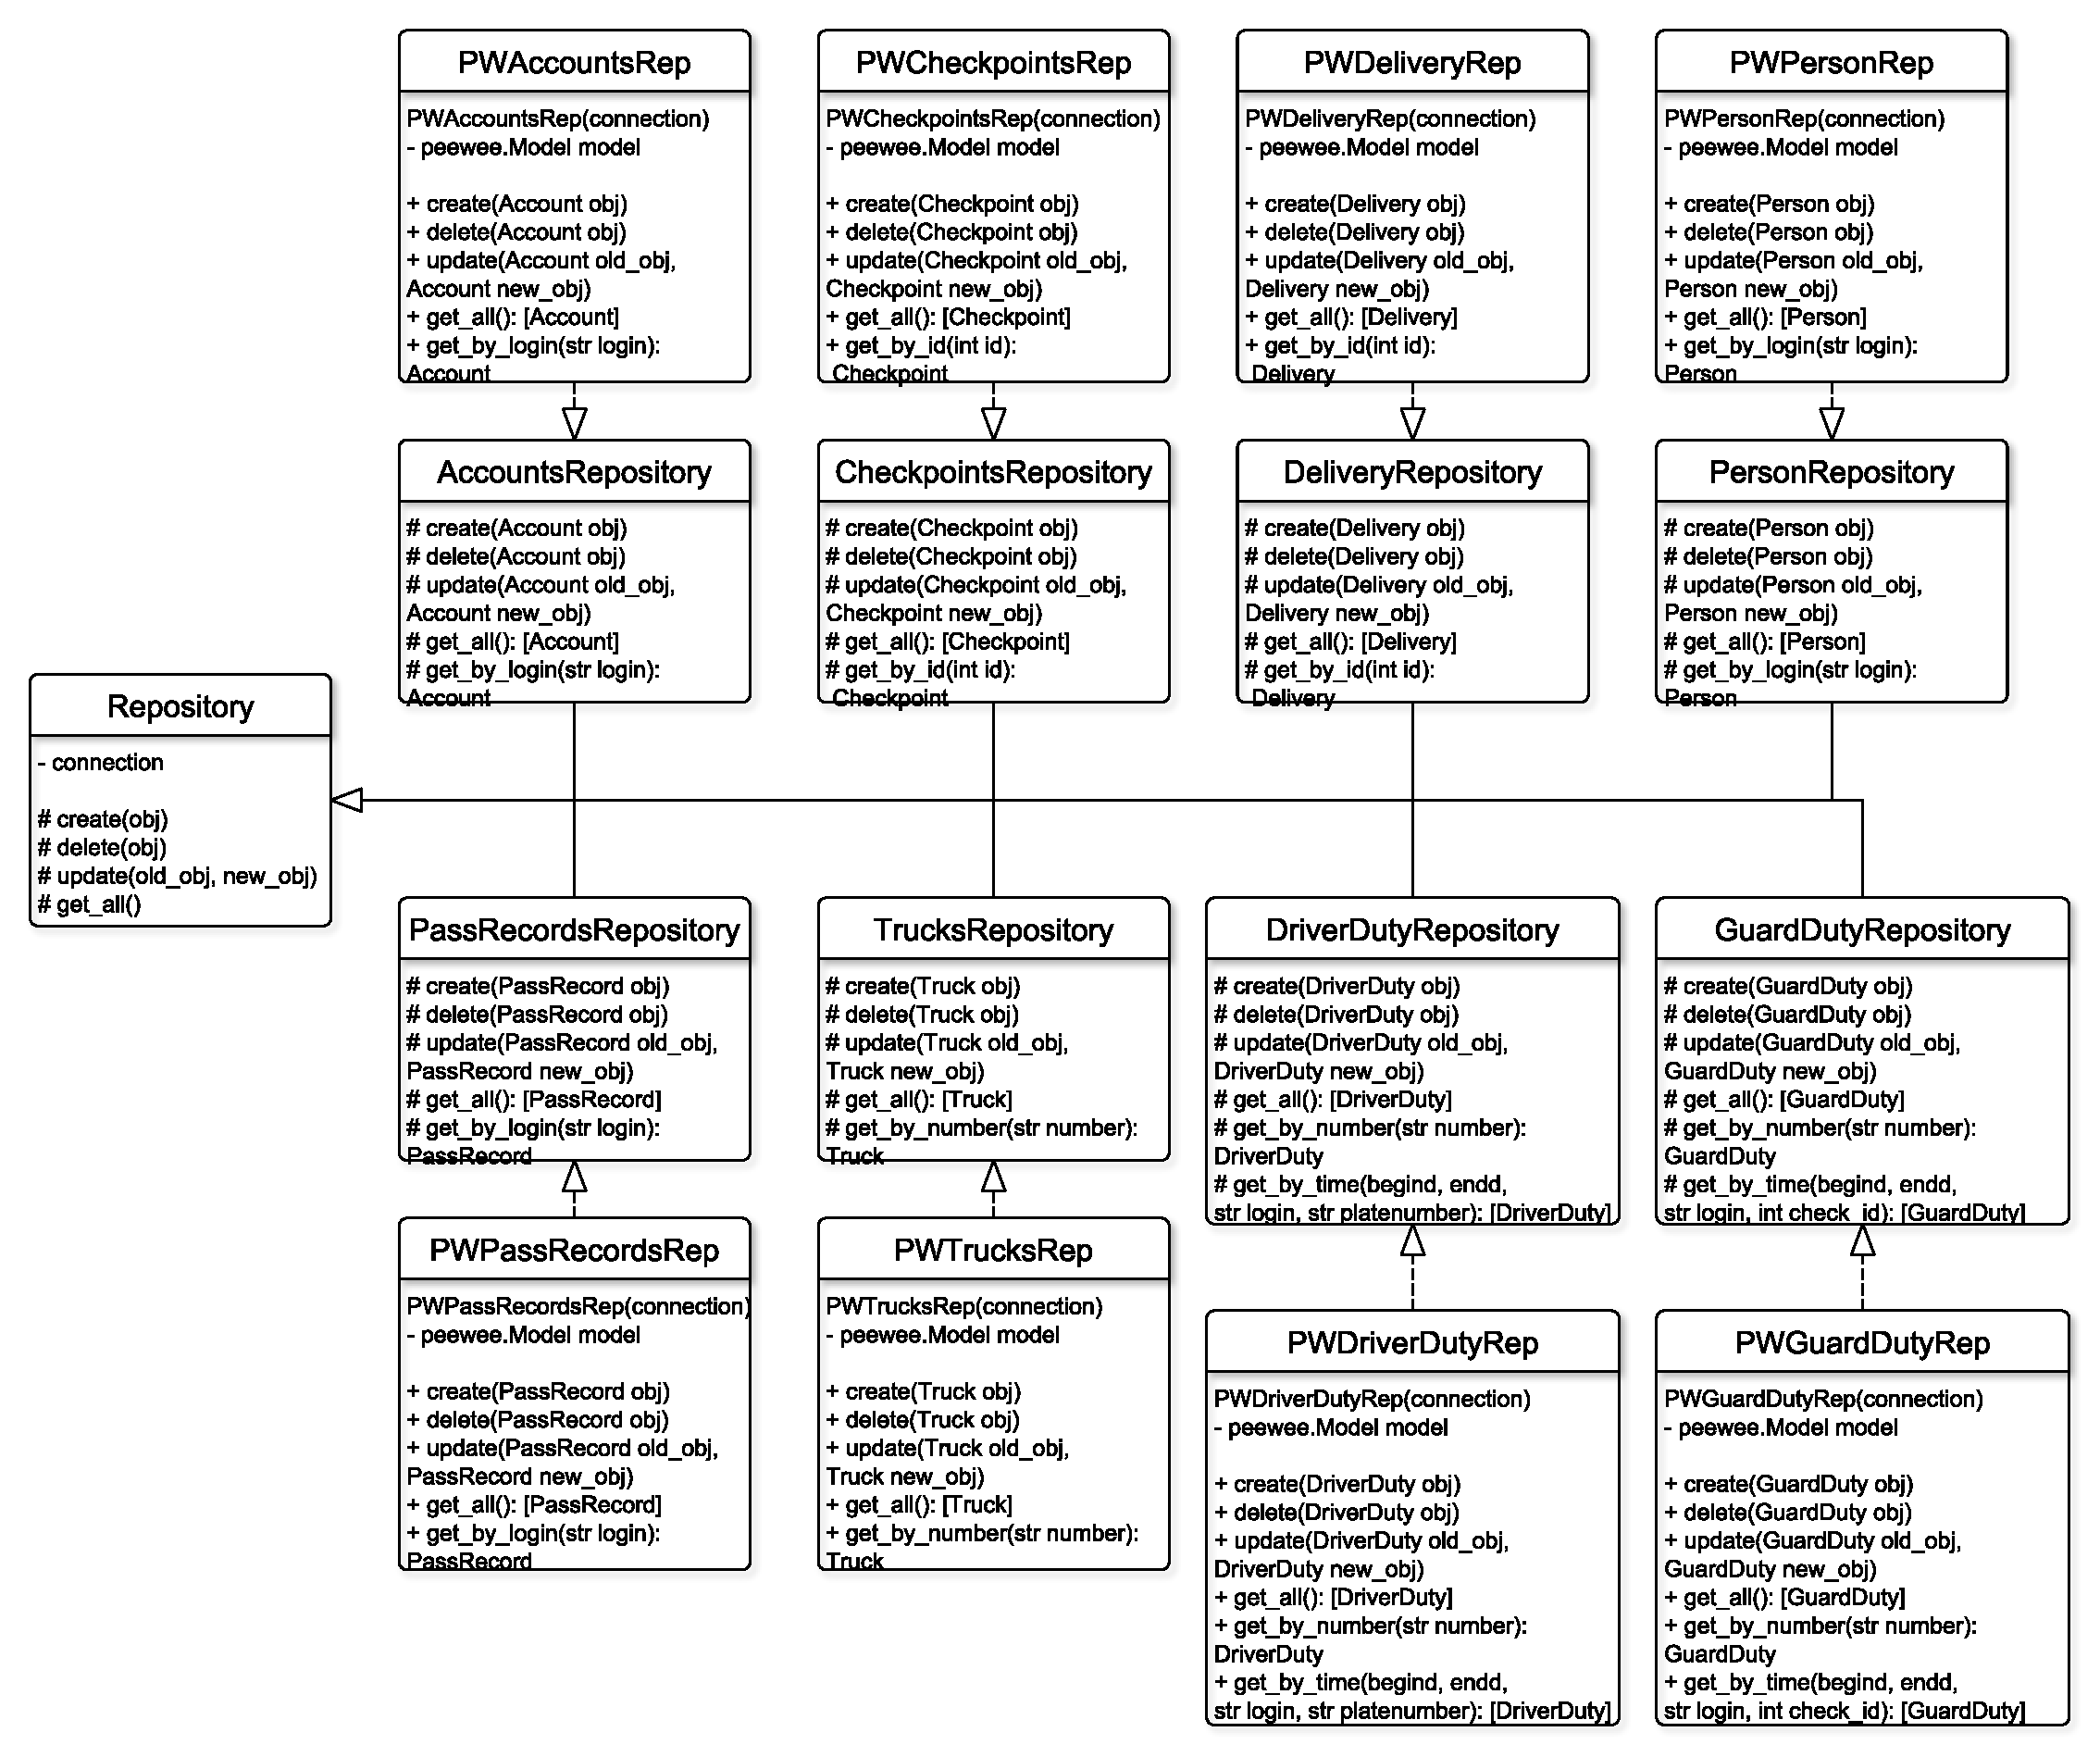
\includegraphics[height=14cm, width = 14cm]{uml/repsoitory.pdf}}
		{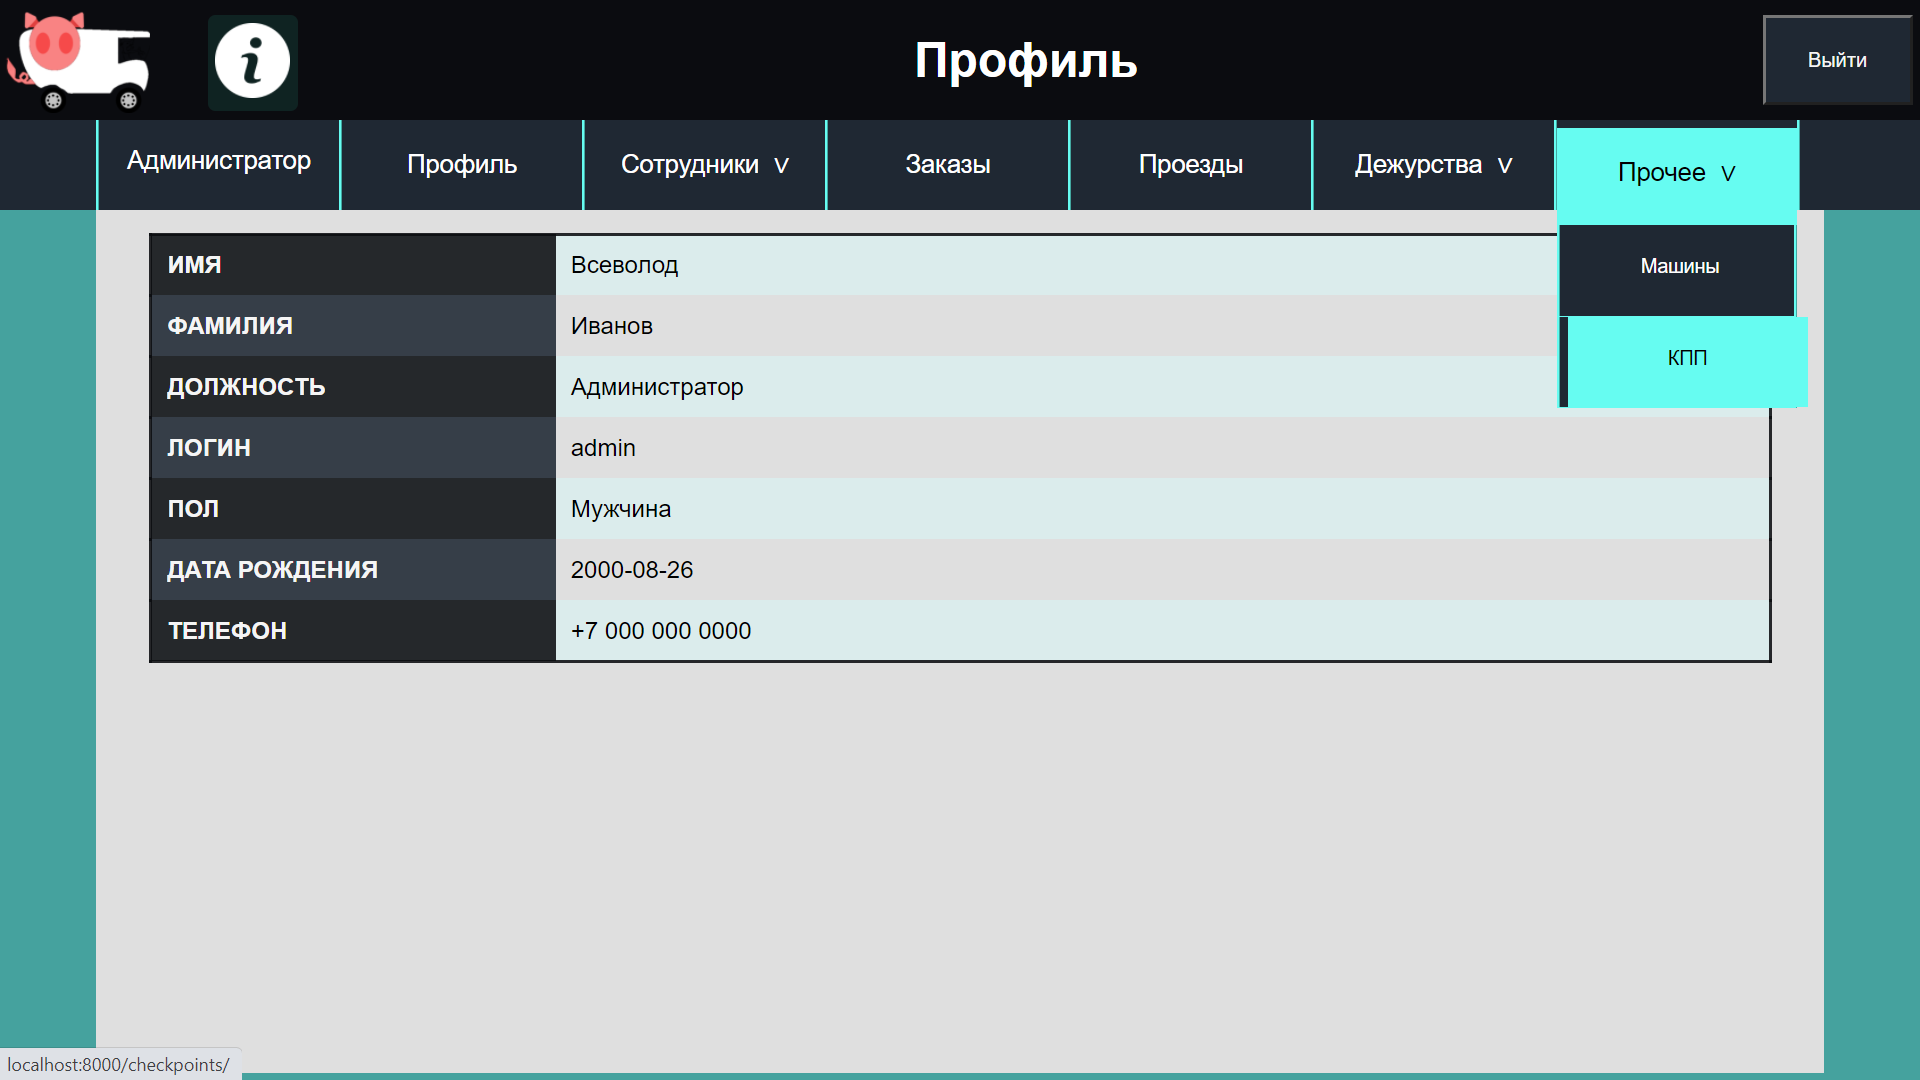
\includegraphics[scale=0.45, angle=0]{sc/admin_profile}}
		\caption{Страница профиля администратора}
	\end{center}
\end{figure}

\begin{figure}[h!] \label{all_profiles_sc}
	\begin{center}
		%		{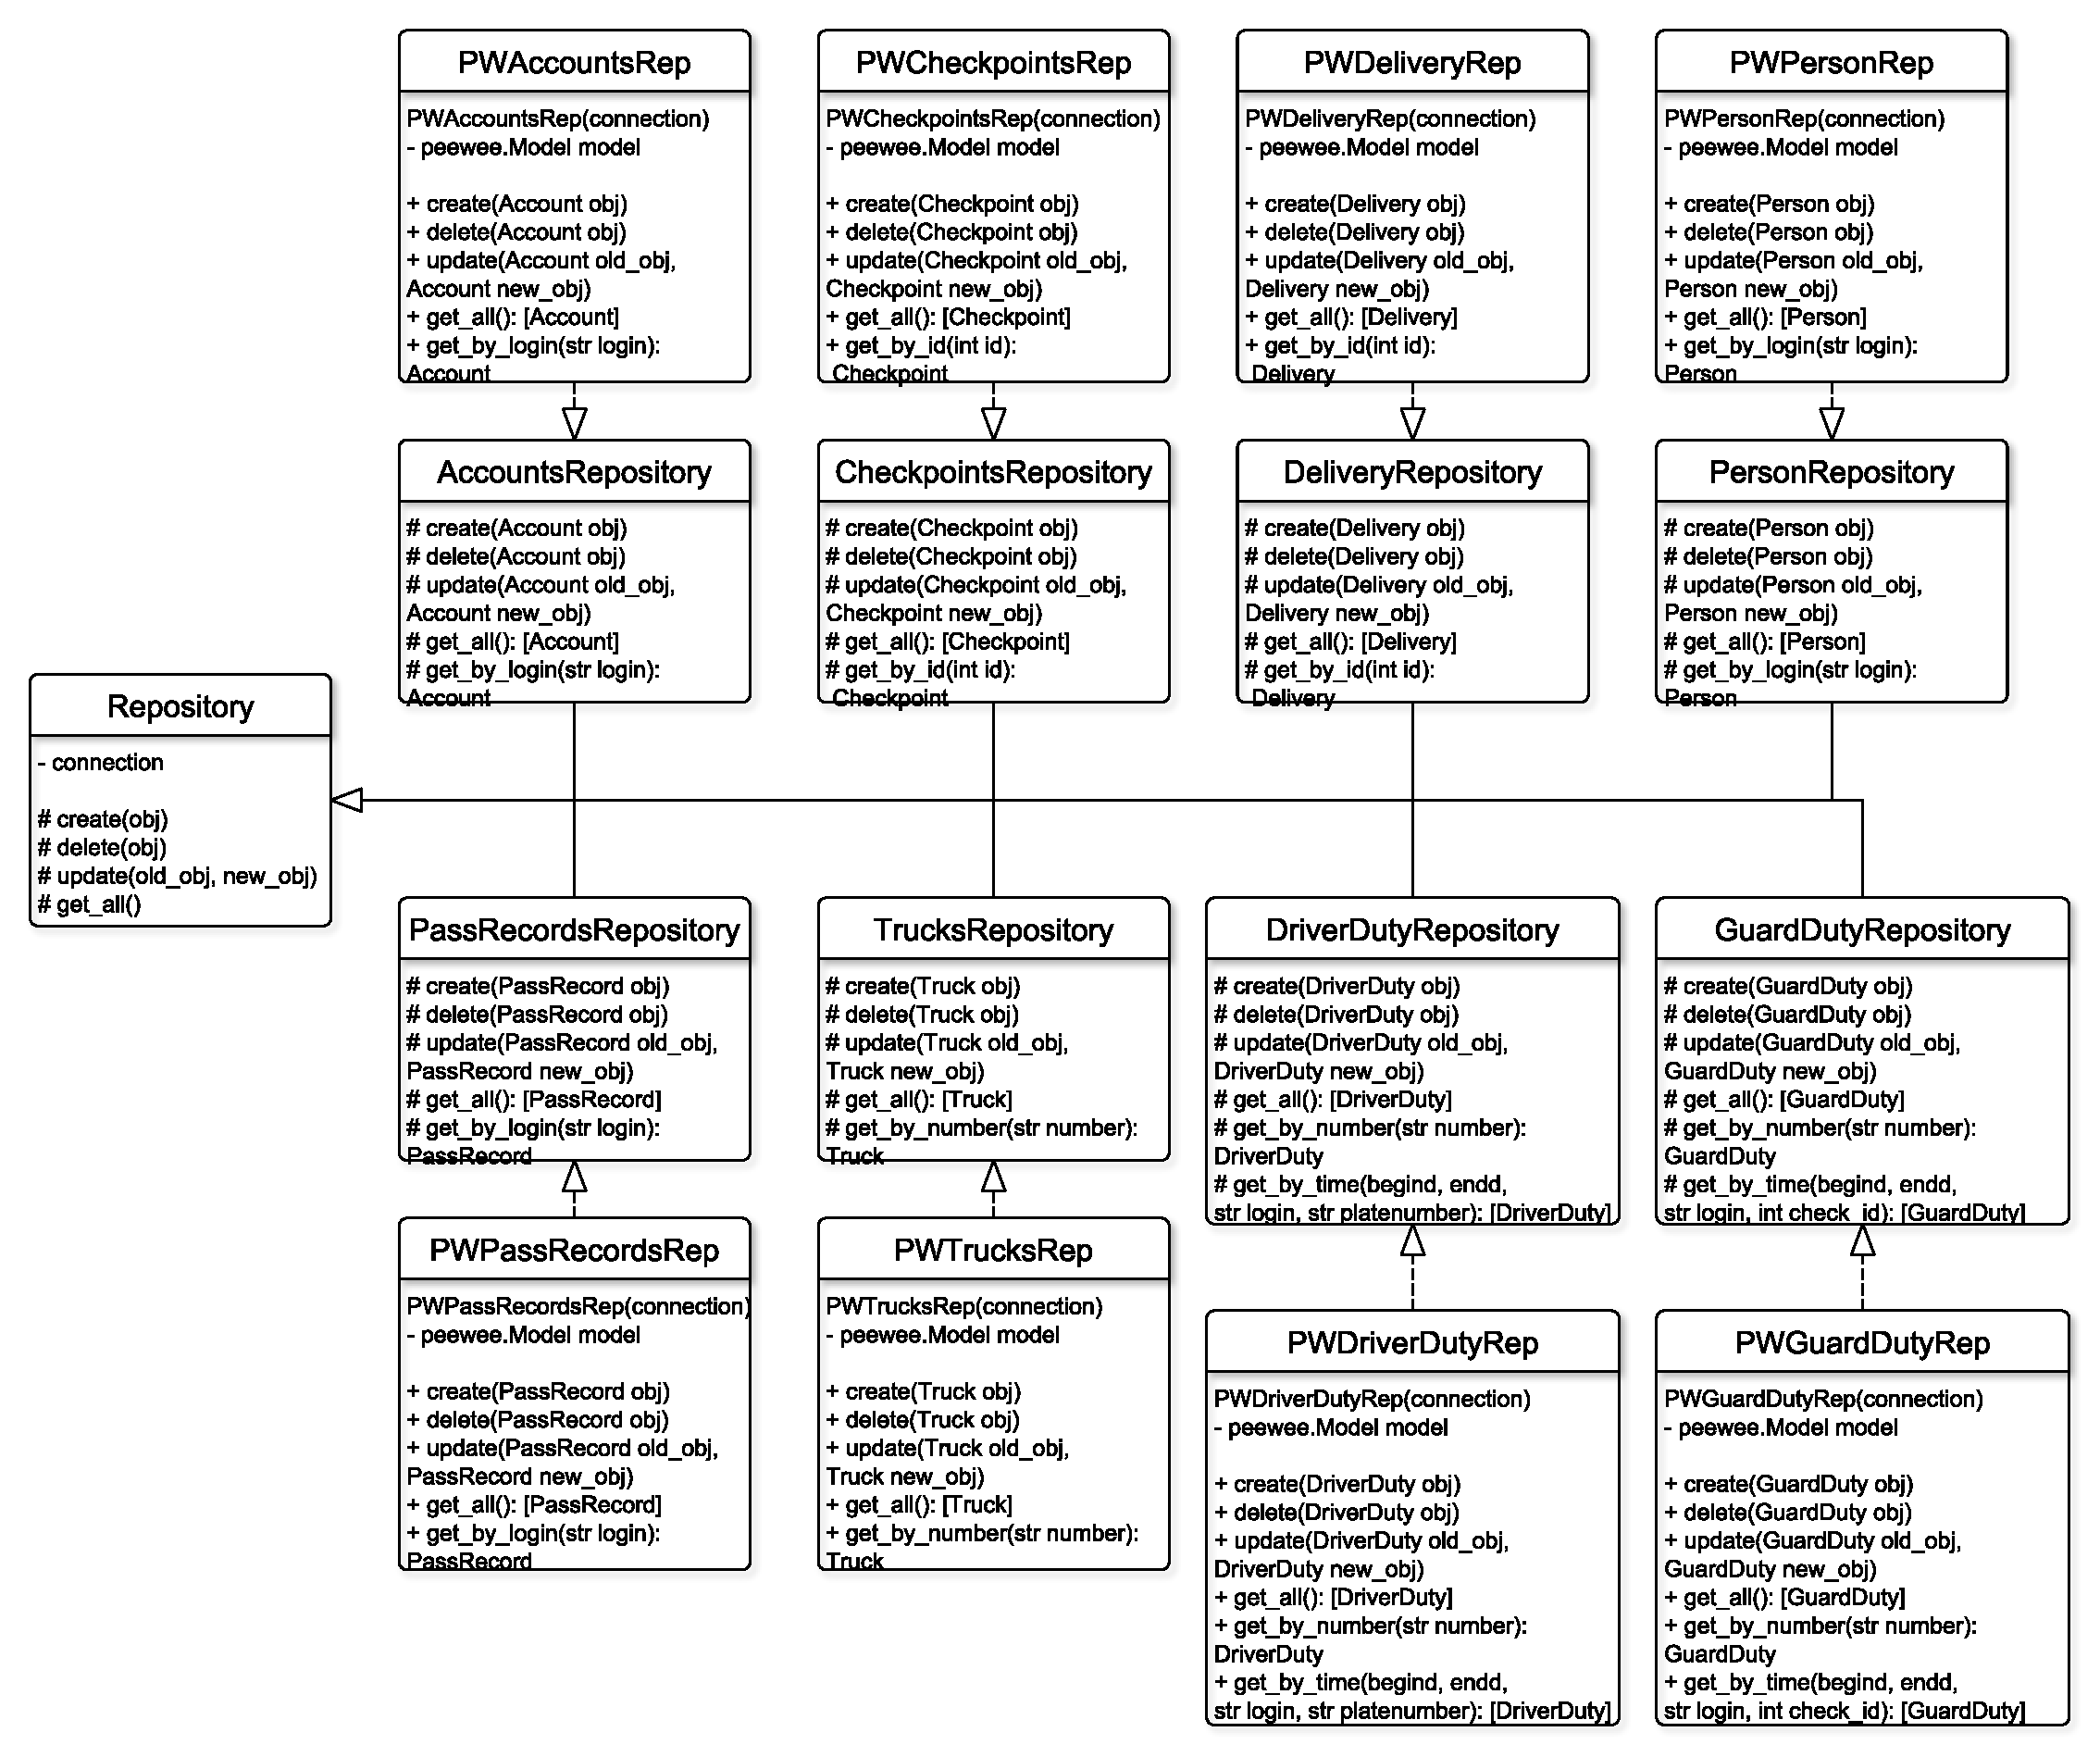
\includegraphics[height=14cm, width = 14cm]{uml/repsoitory.pdf}}
		{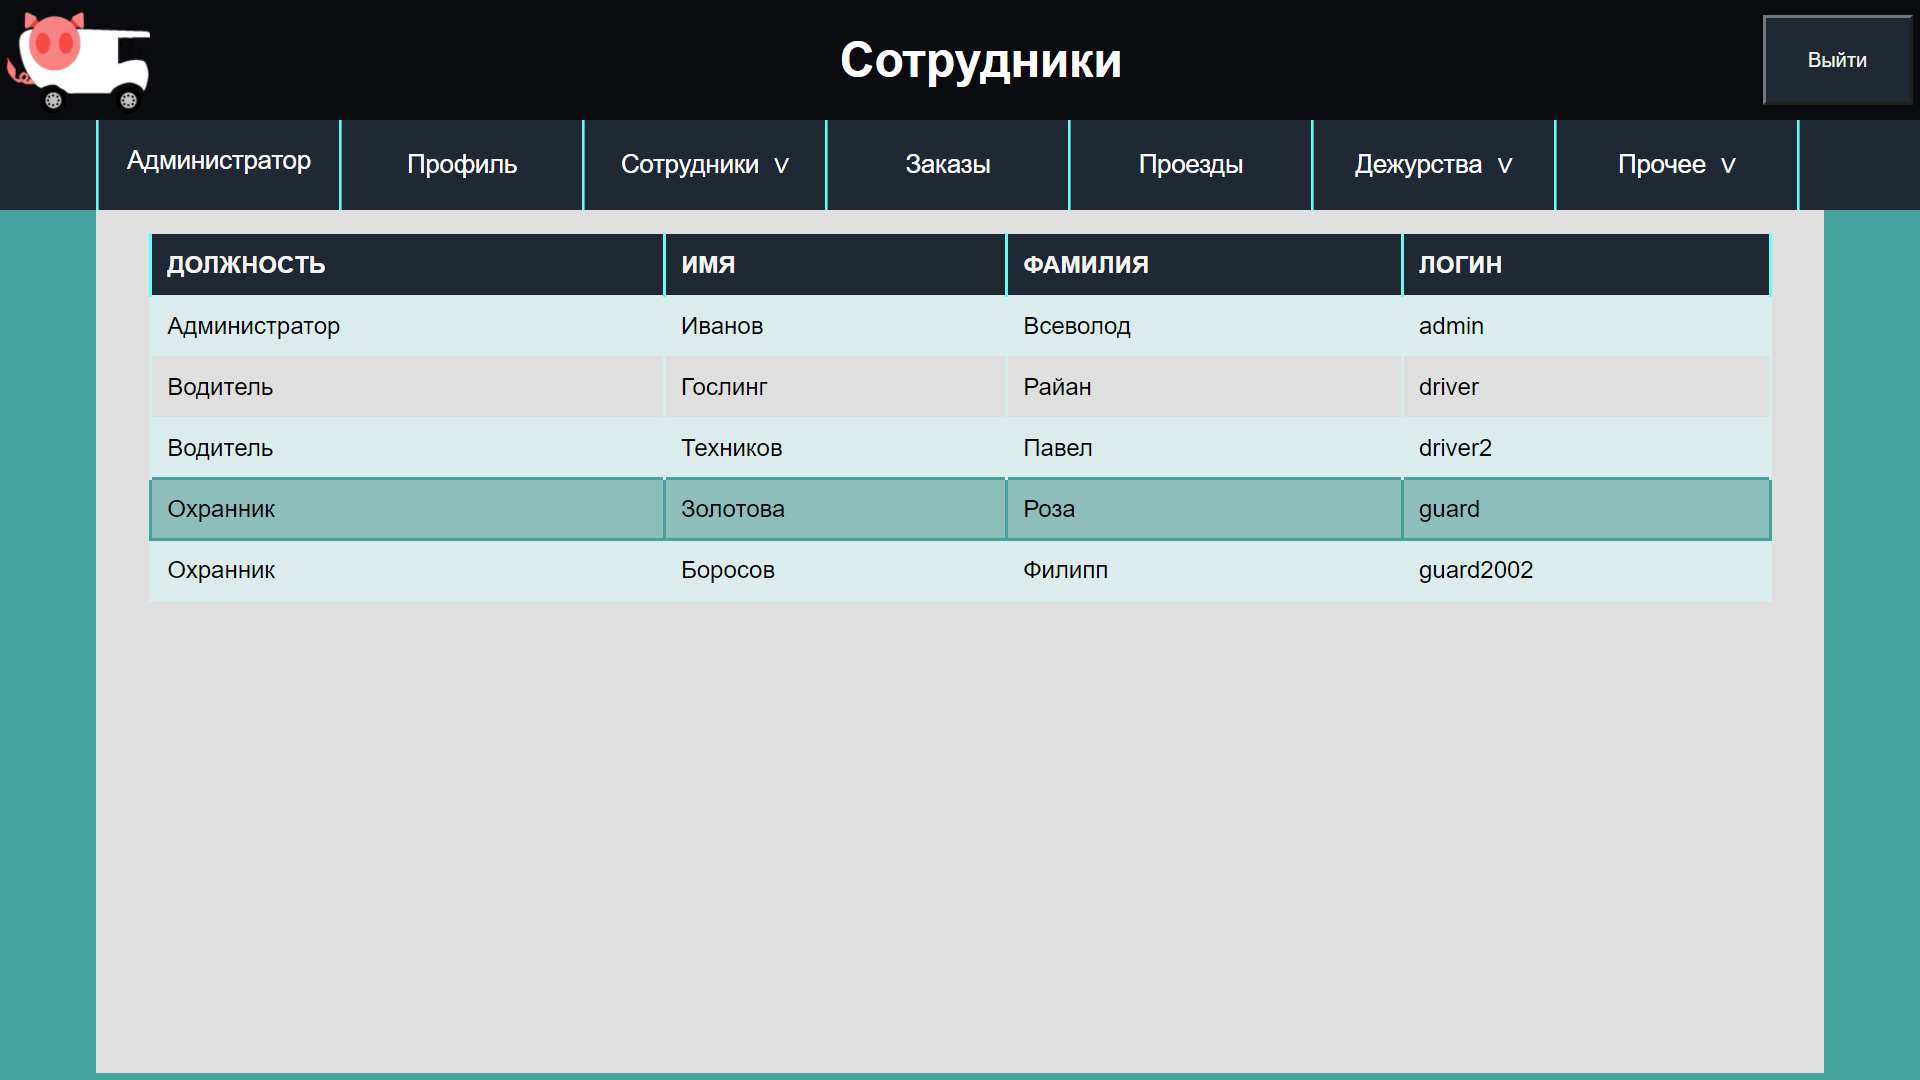
\includegraphics[scale=0.43, angle=0]{sc/all_profiles}}
		\caption{Страница просмотра всех сотрудников}
	\end{center}
\end{figure}

\begin{figure}[h!] \label{unver_sc}
	\begin{center}
		%		{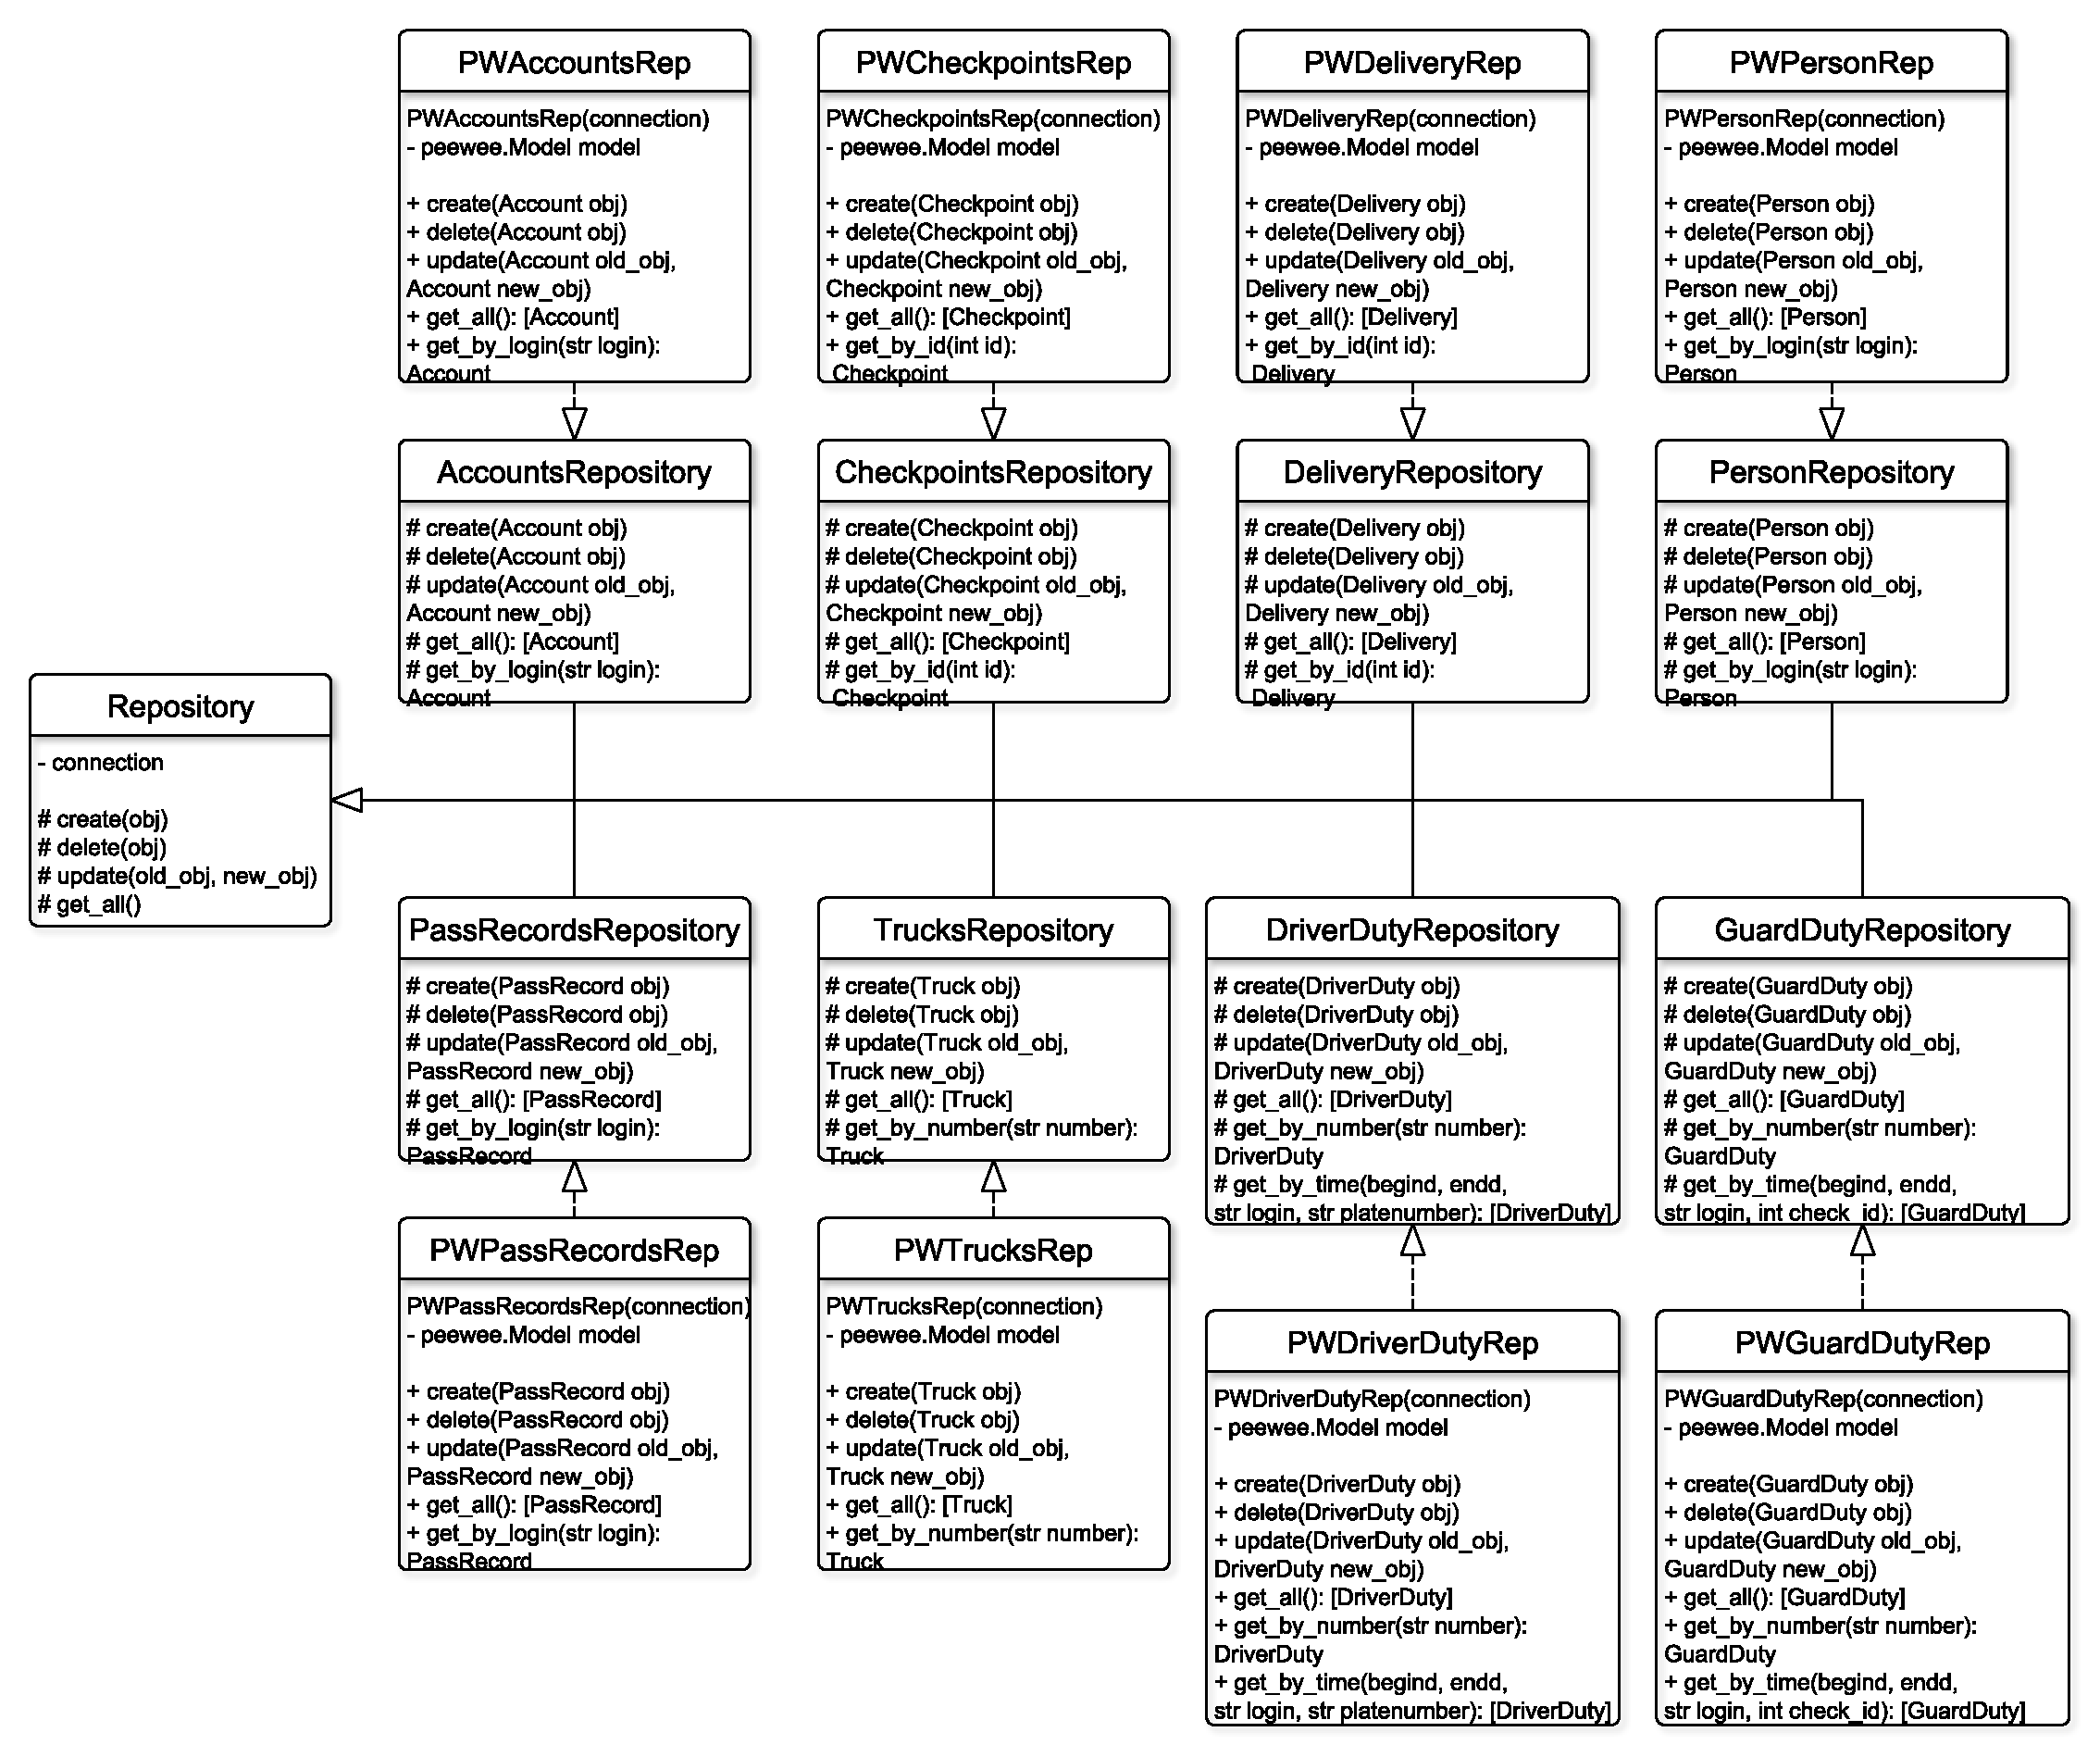
\includegraphics[height=14cm, width = 14cm]{uml/repsoitory.pdf}}
		{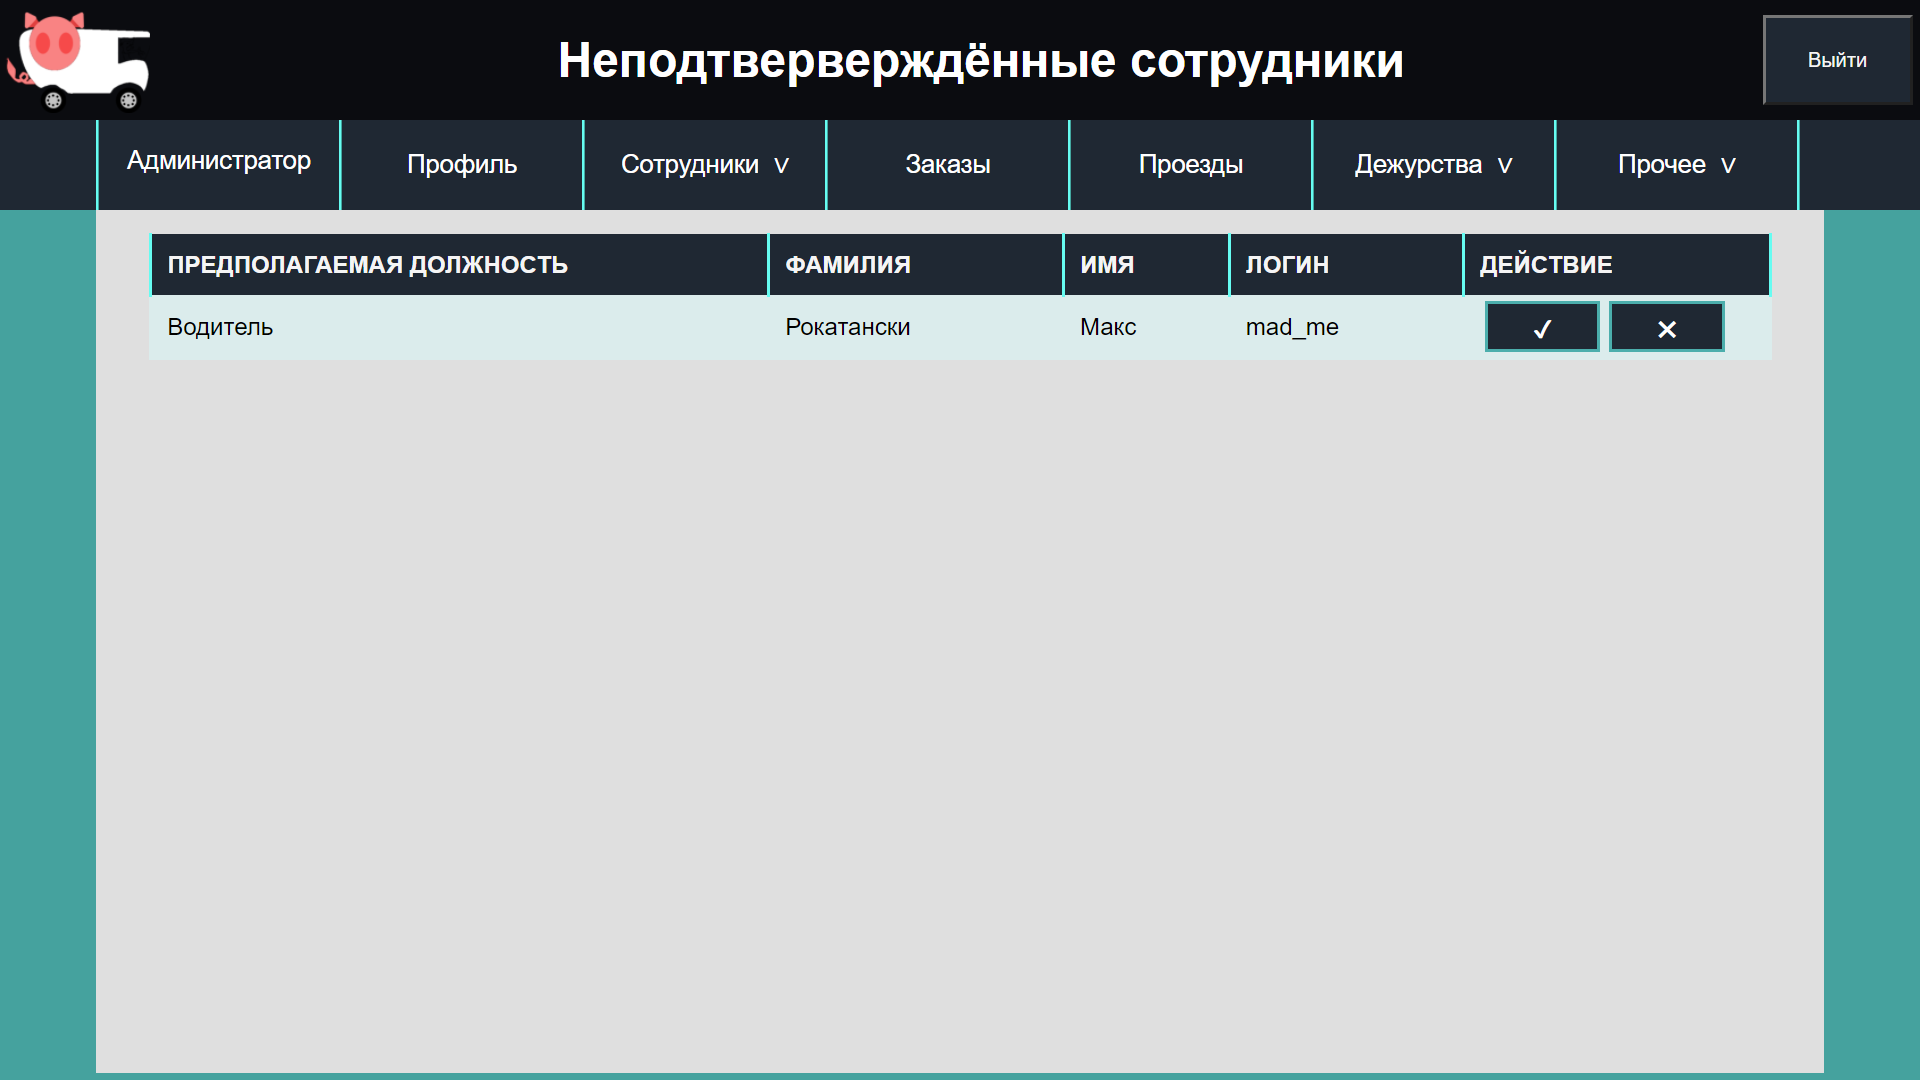
\includegraphics[scale=0.43, angle=0]{sc/unver}}
		\caption{Страница просмотра заявок регистрации}
	\end{center}
\end{figure}

\begin{figure}[h!] \label{all_delivery_sc}
	\begin{center}
		%		{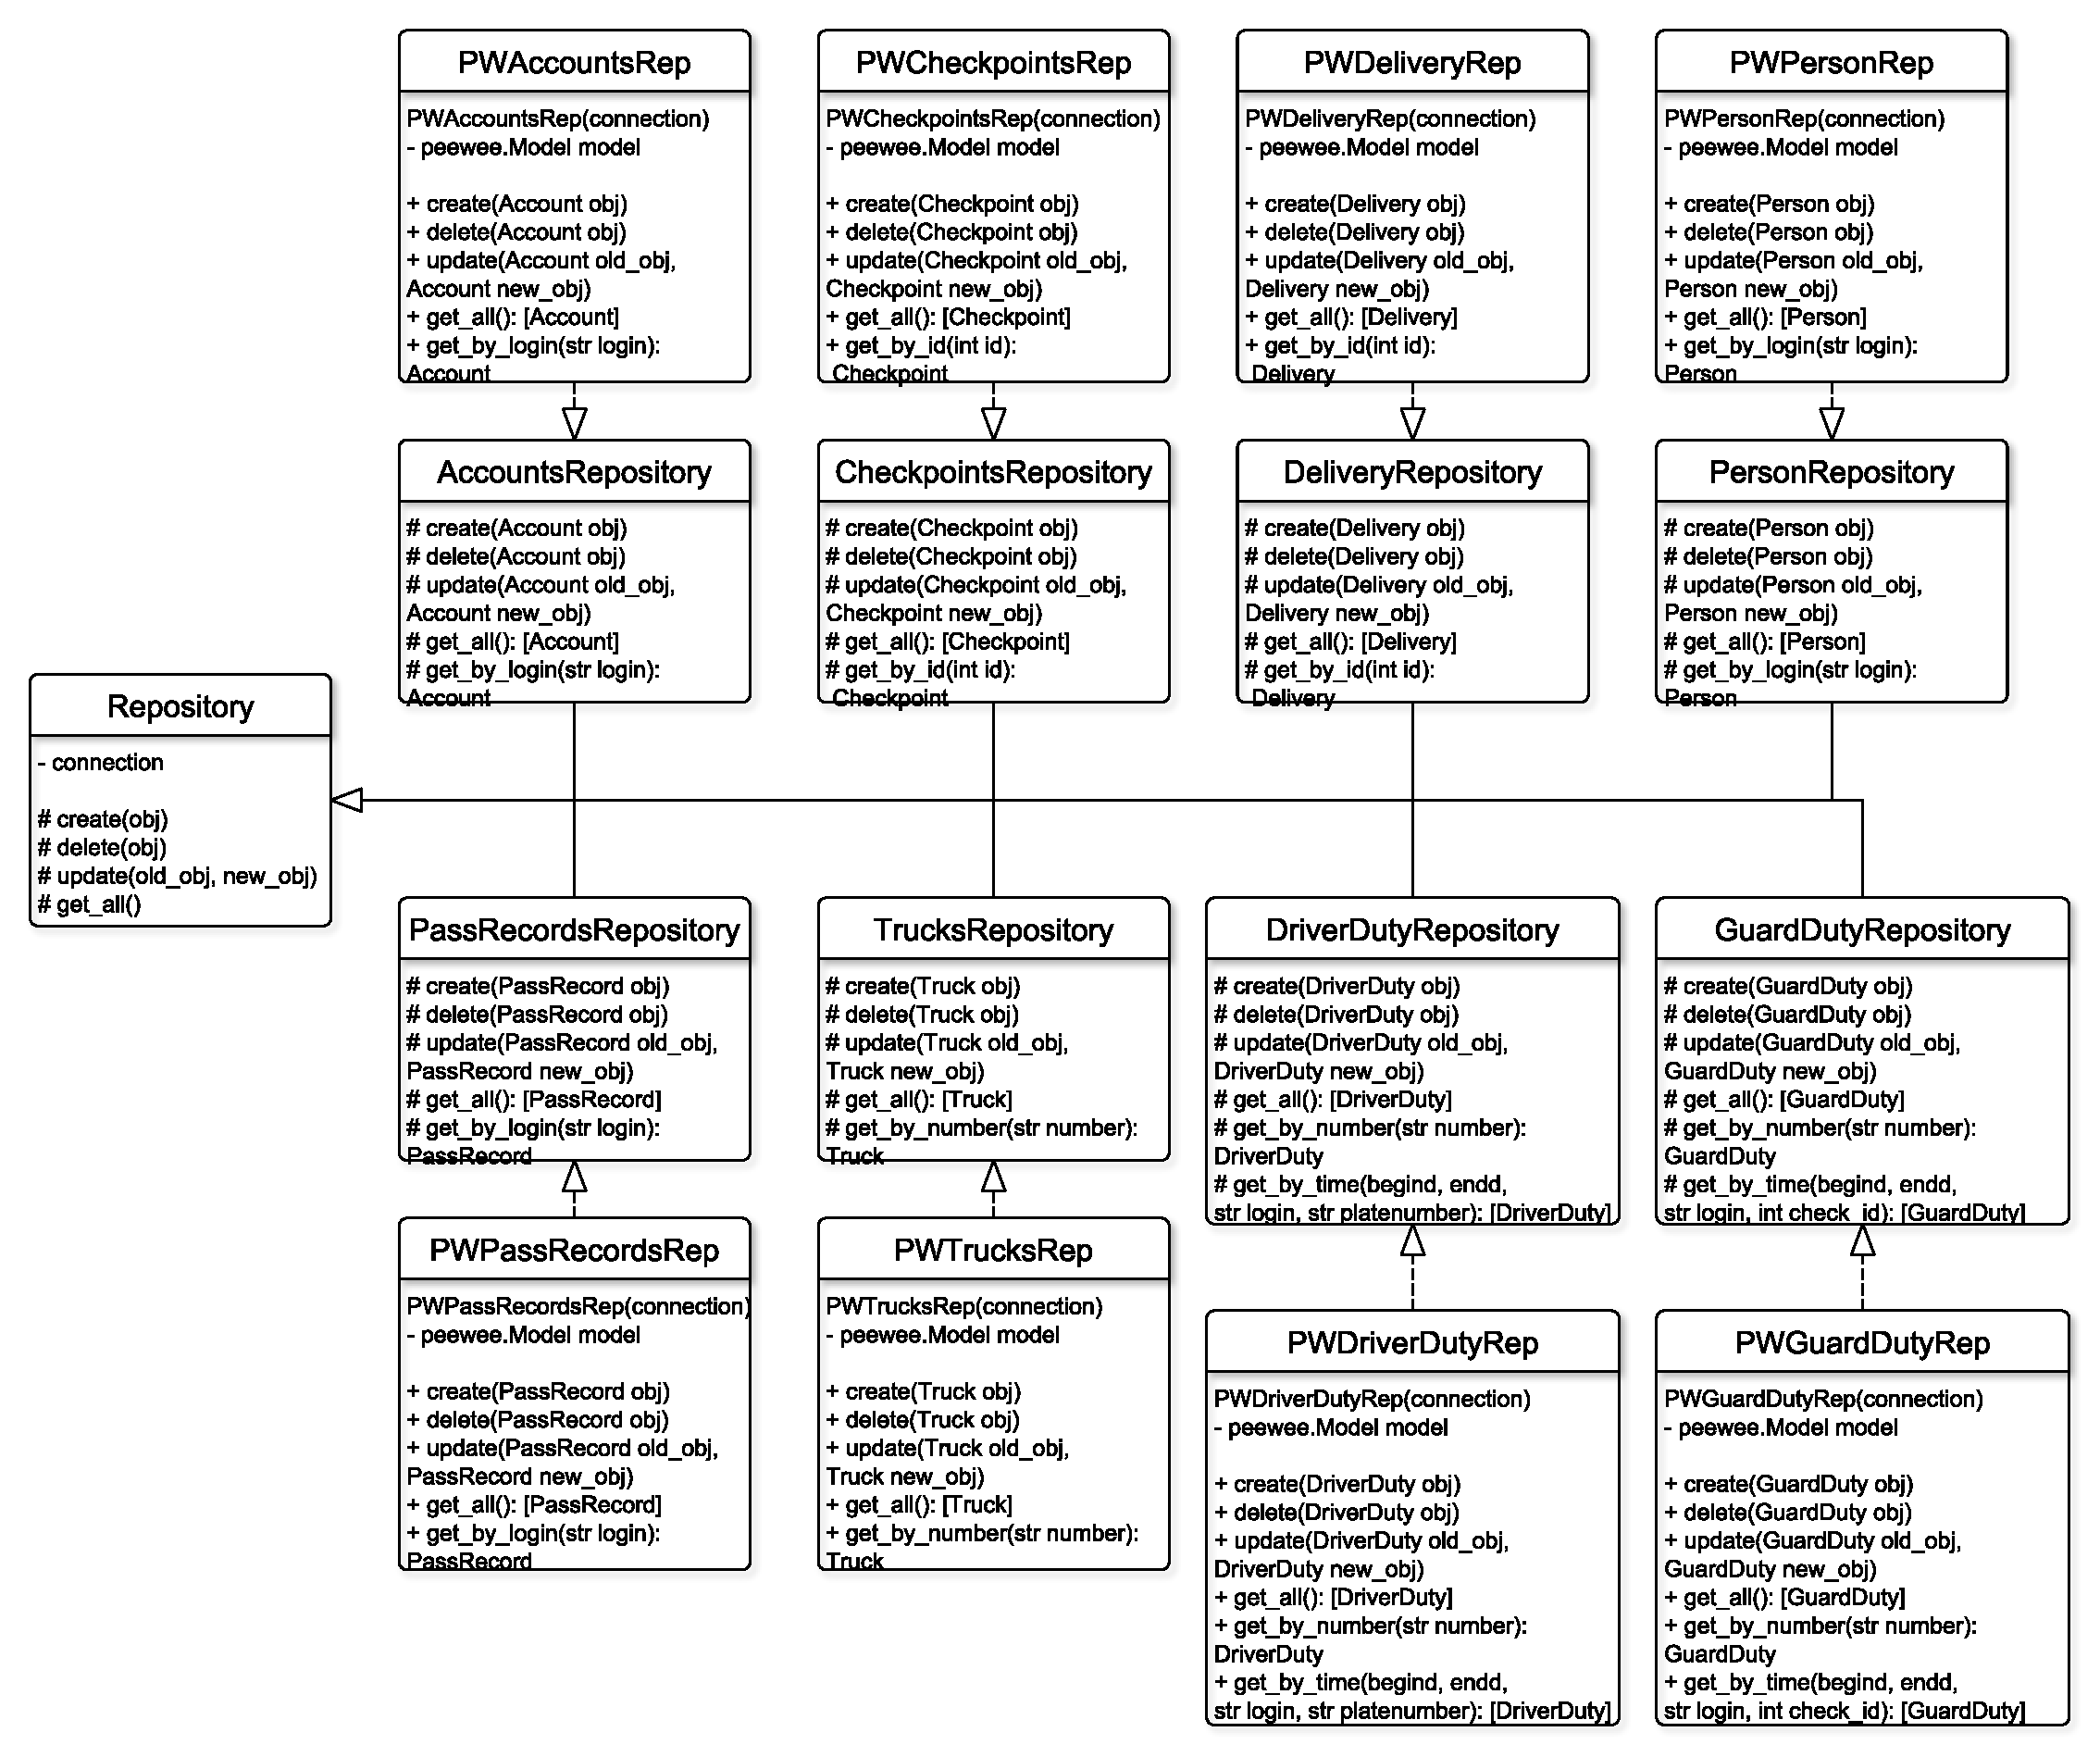
\includegraphics[height=14cm, width = 14cm]{uml/repsoitory.pdf}}
		{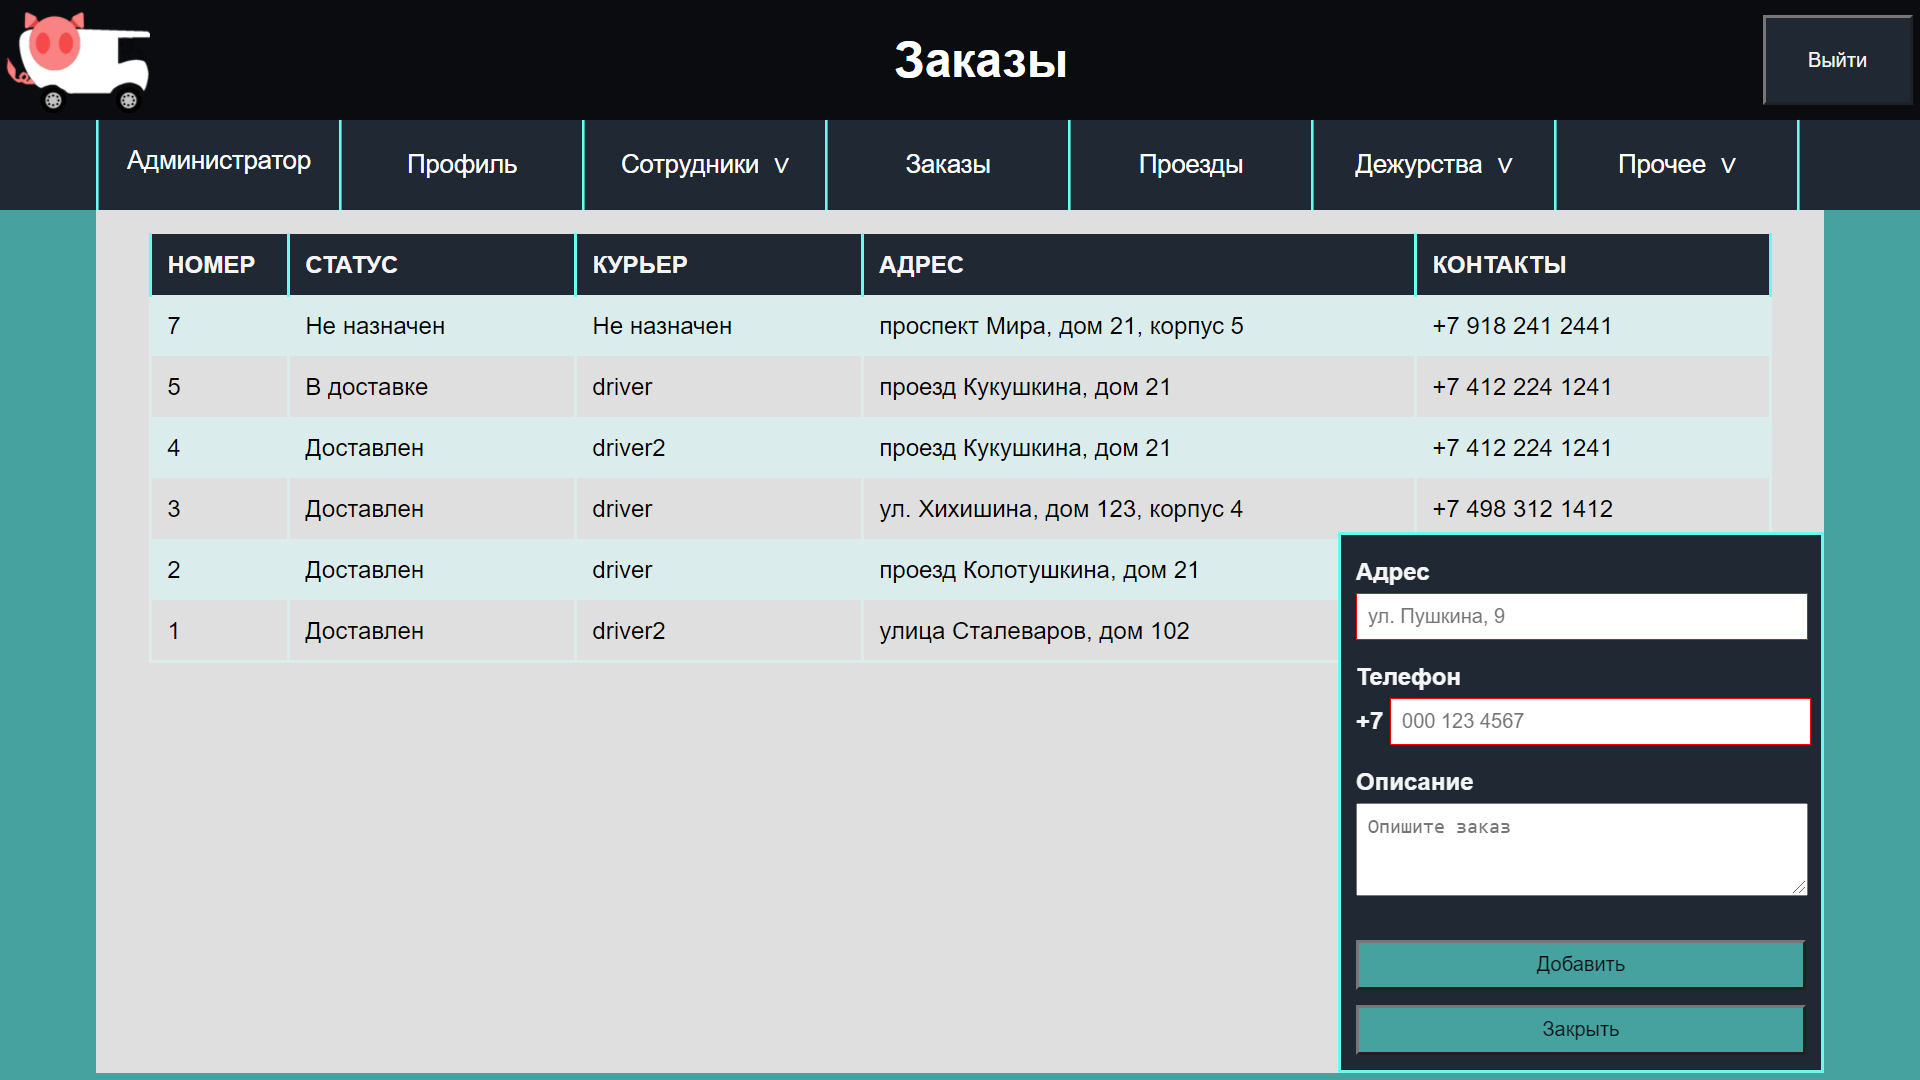
\includegraphics[scale=0.43, angle=0]{sc/all_delivery}}
		\caption{Страница просмотра и создания заказов}
	\end{center}
\end{figure}

\begin{figure}[h!] \label{all_pass_sc}
	\begin{center}
		%		{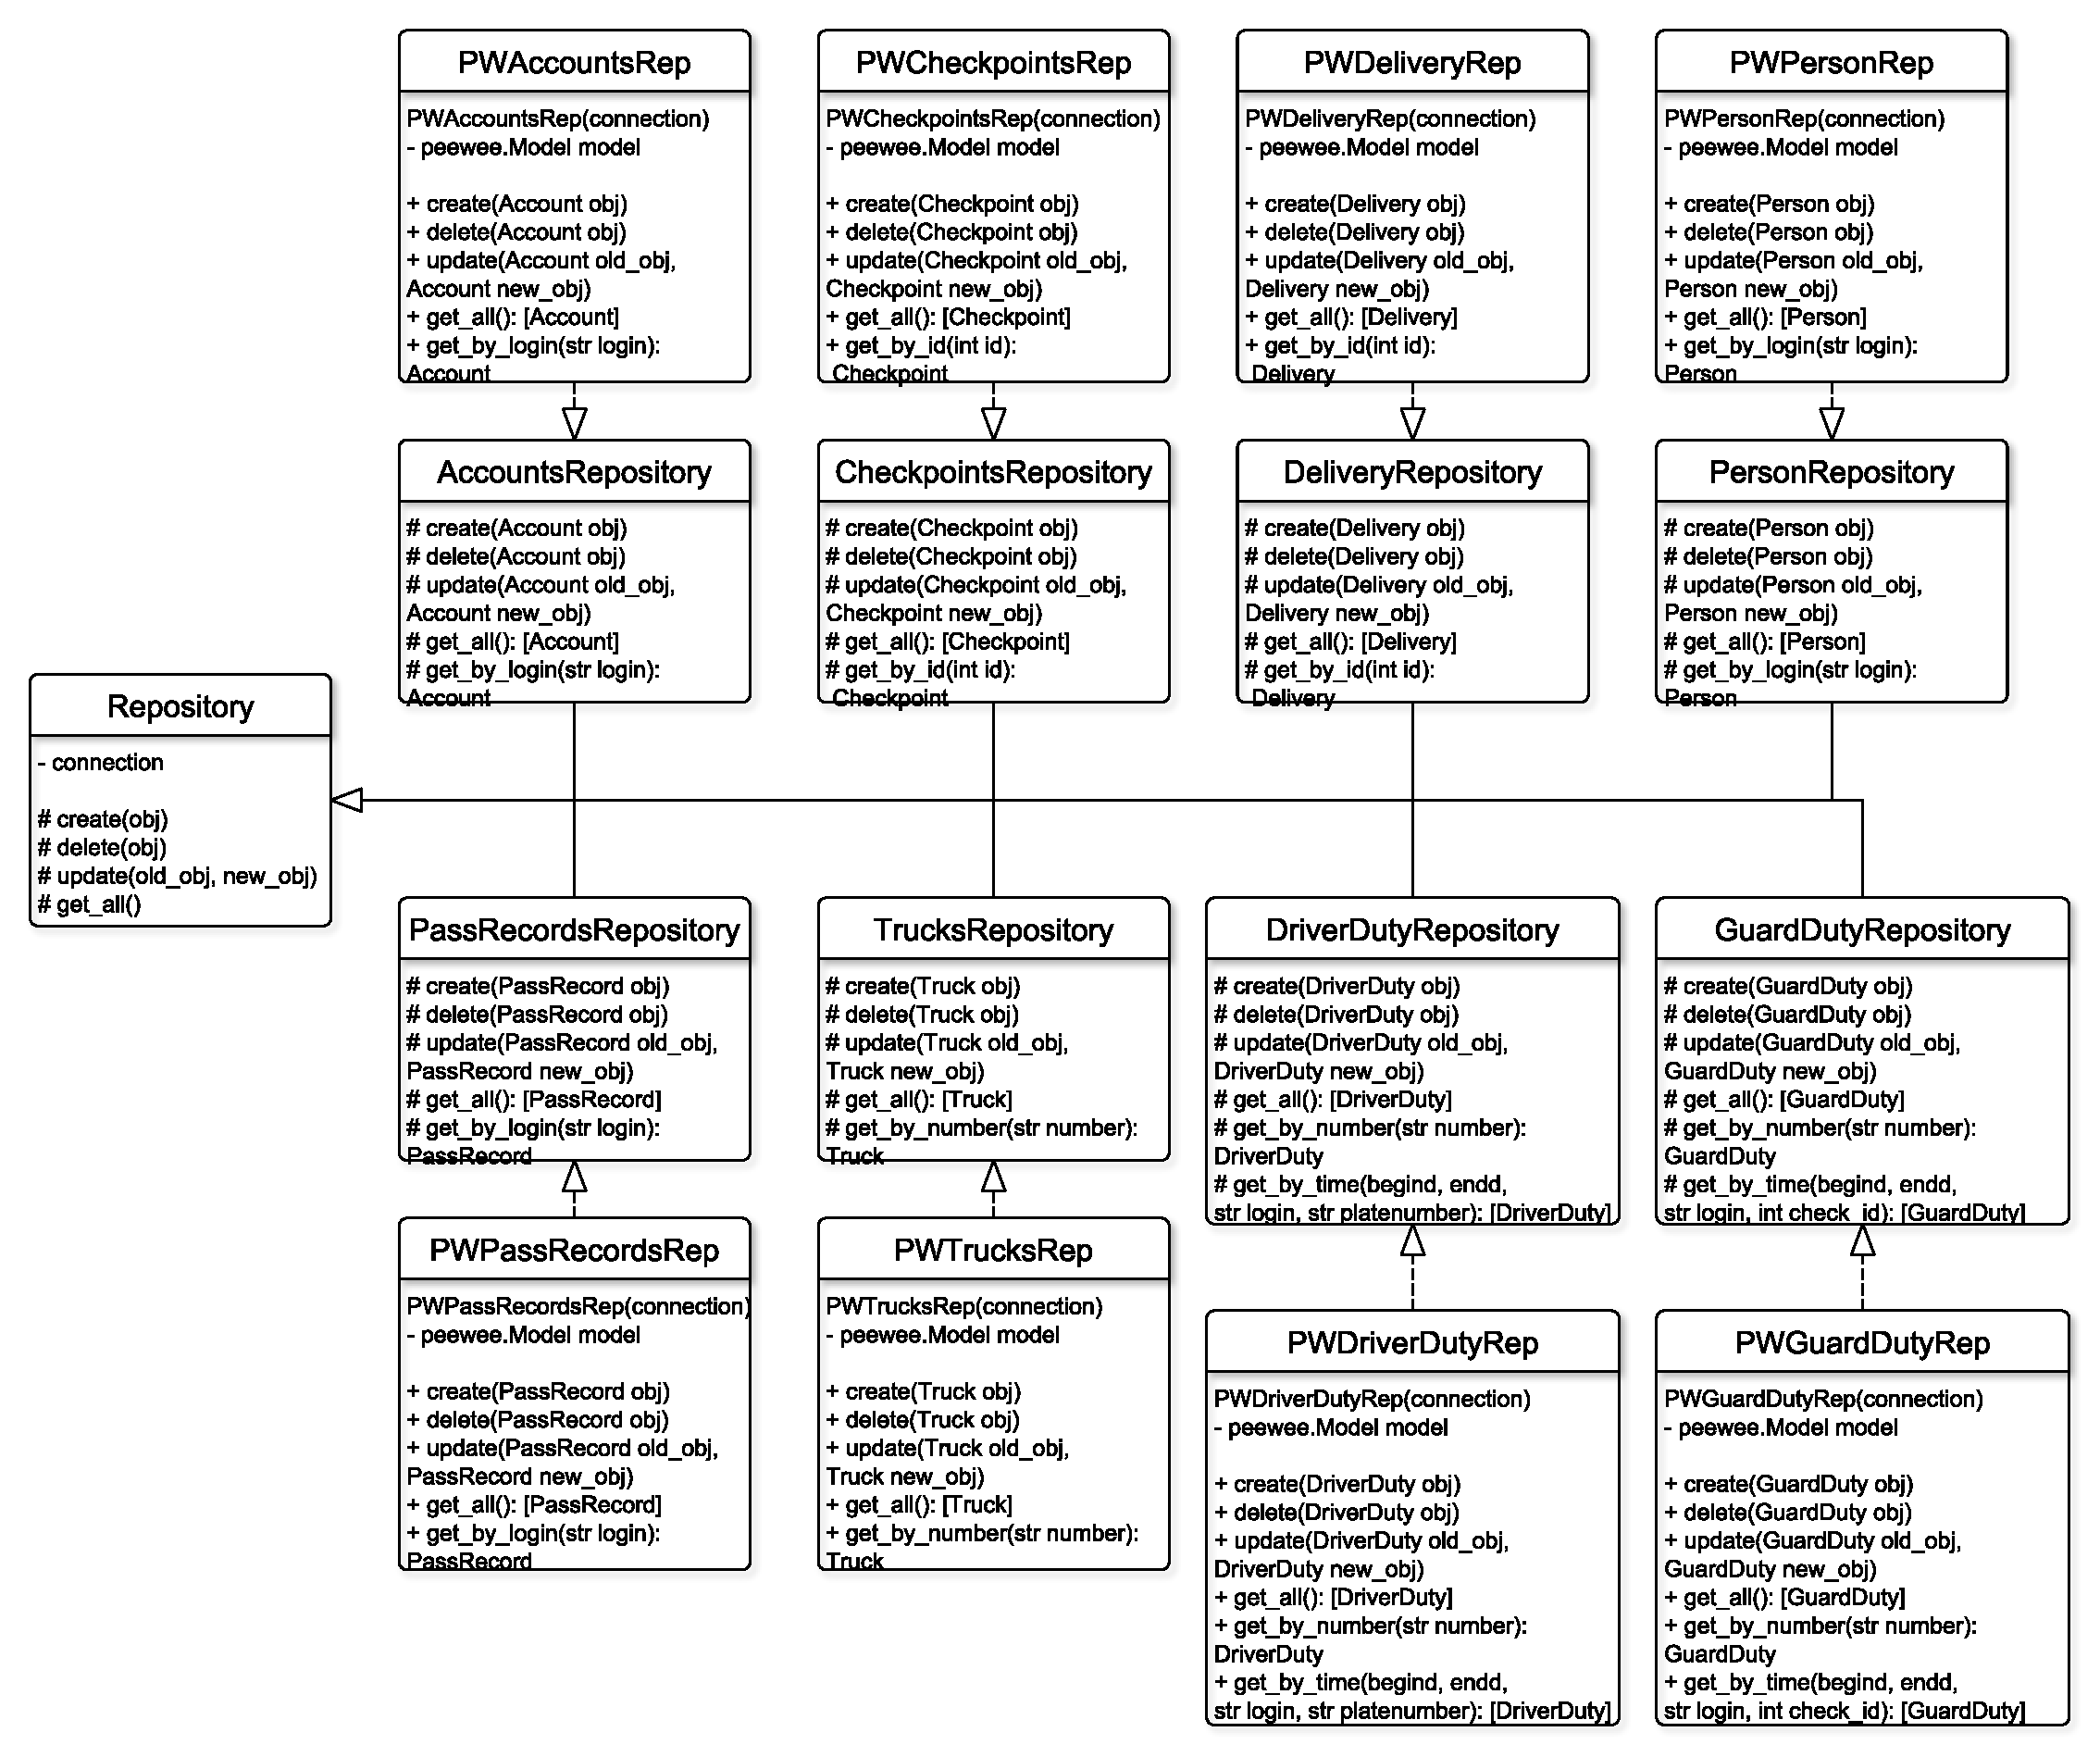
\includegraphics[height=14cm, width = 14cm]{uml/repsoitory.pdf}}
		{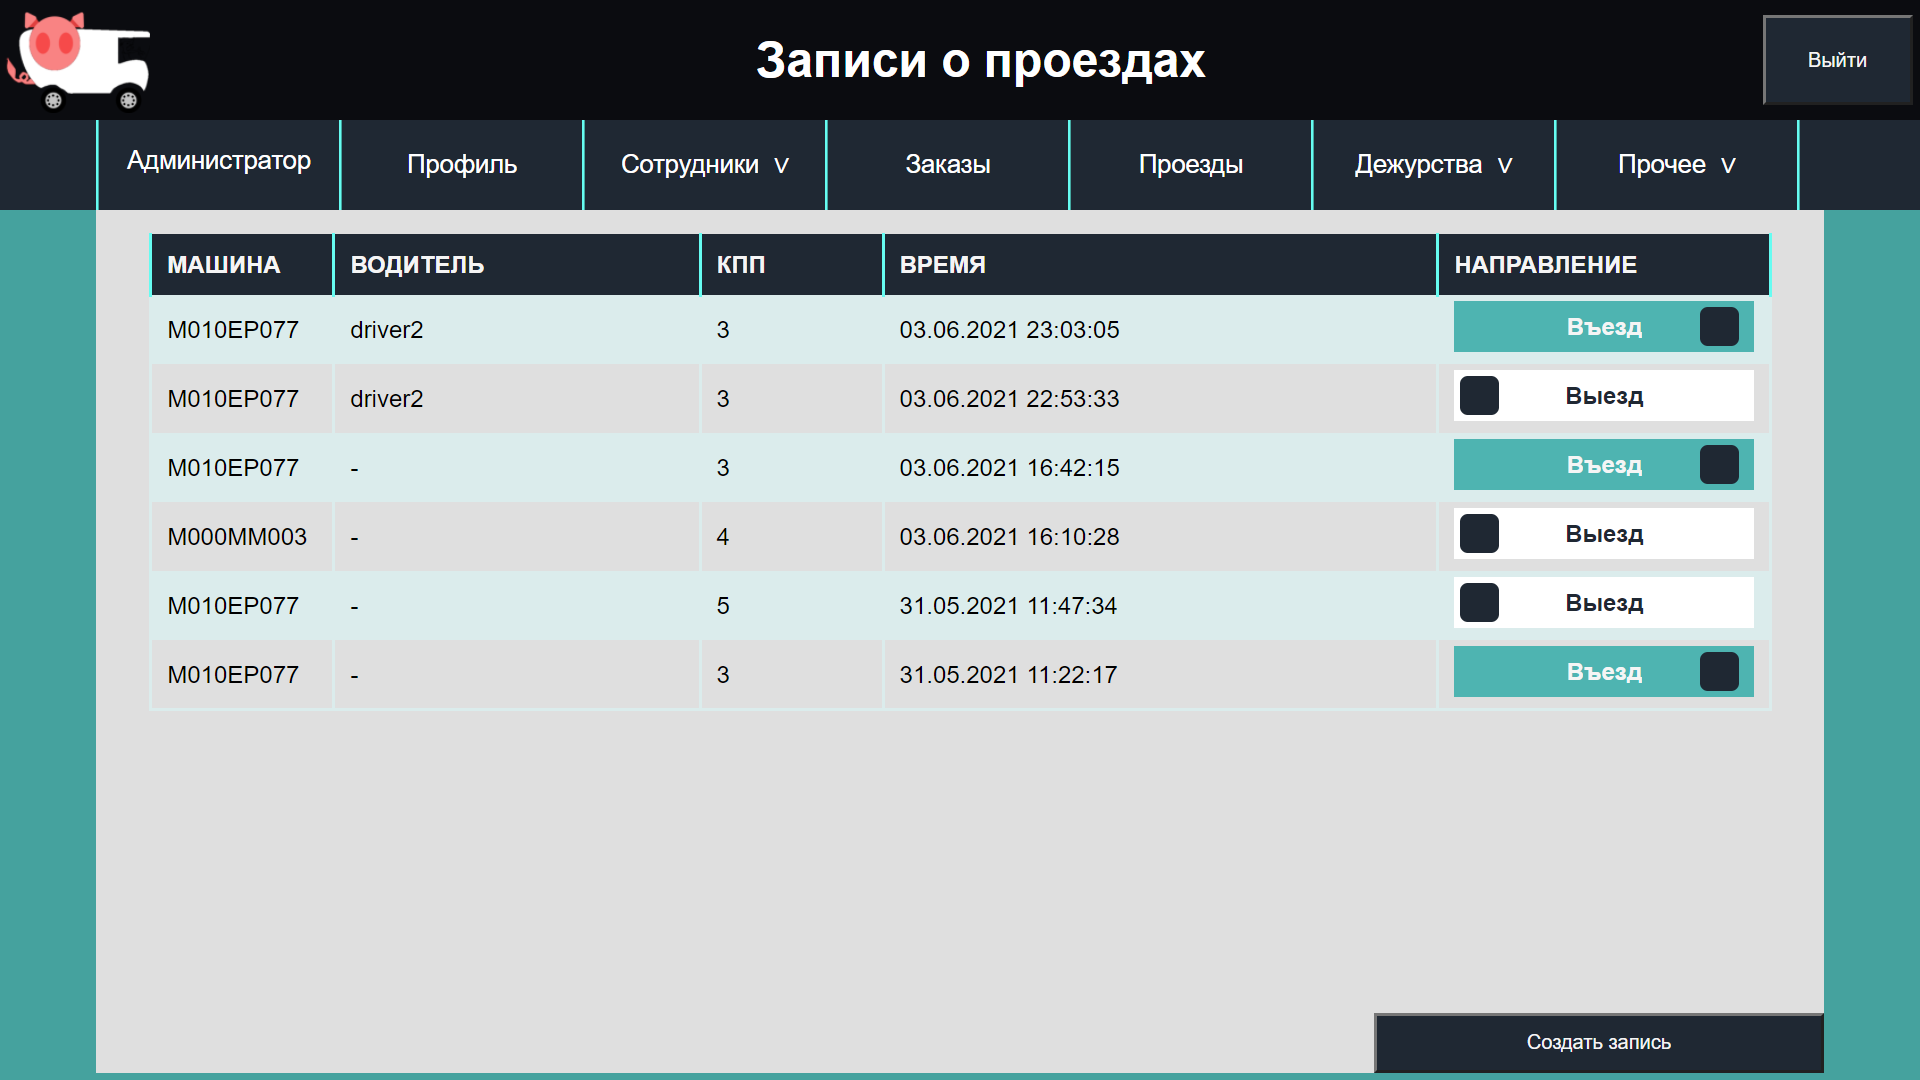
\includegraphics[scale=0.43, angle=0]{sc/all_pass}}
		\caption{Страница просмотра и регистрации записей о проездах}
	\end{center}
\end{figure}

\begin{figure}[h!] \label{driver_duty_sc}
	\begin{center}
		%		{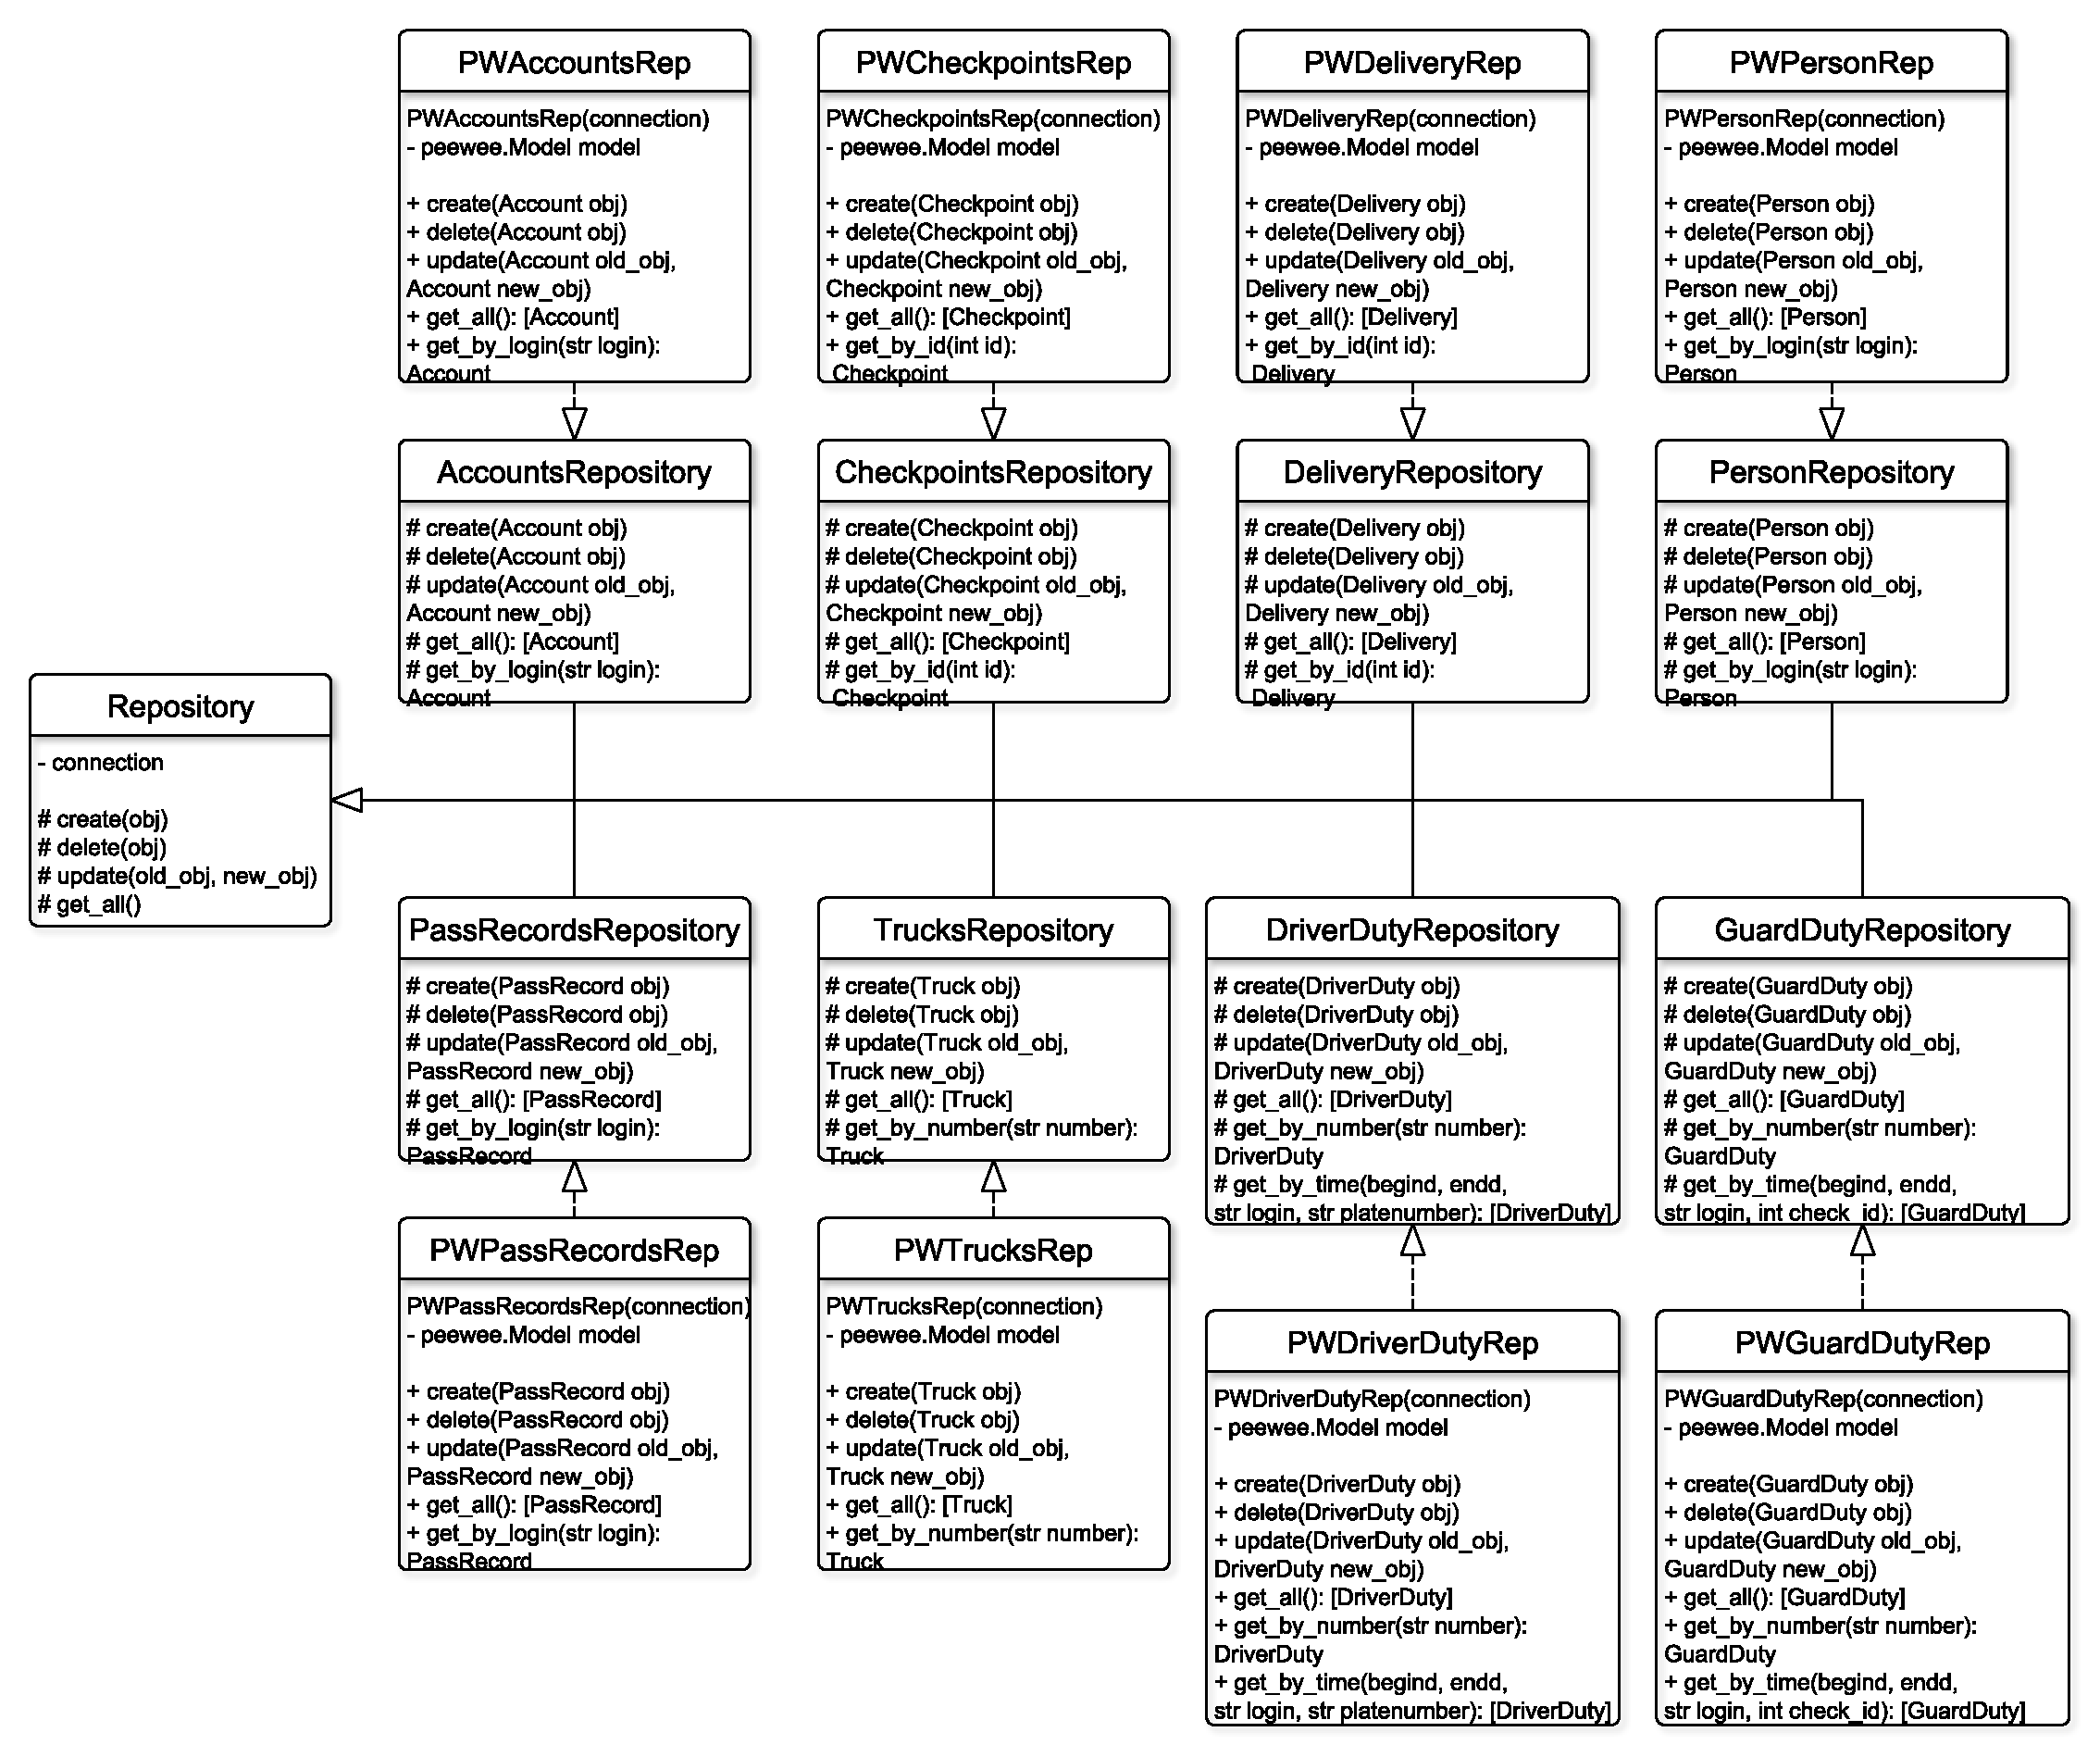
\includegraphics[height=14cm, width = 14cm]{uml/repsoitory.pdf}}
		{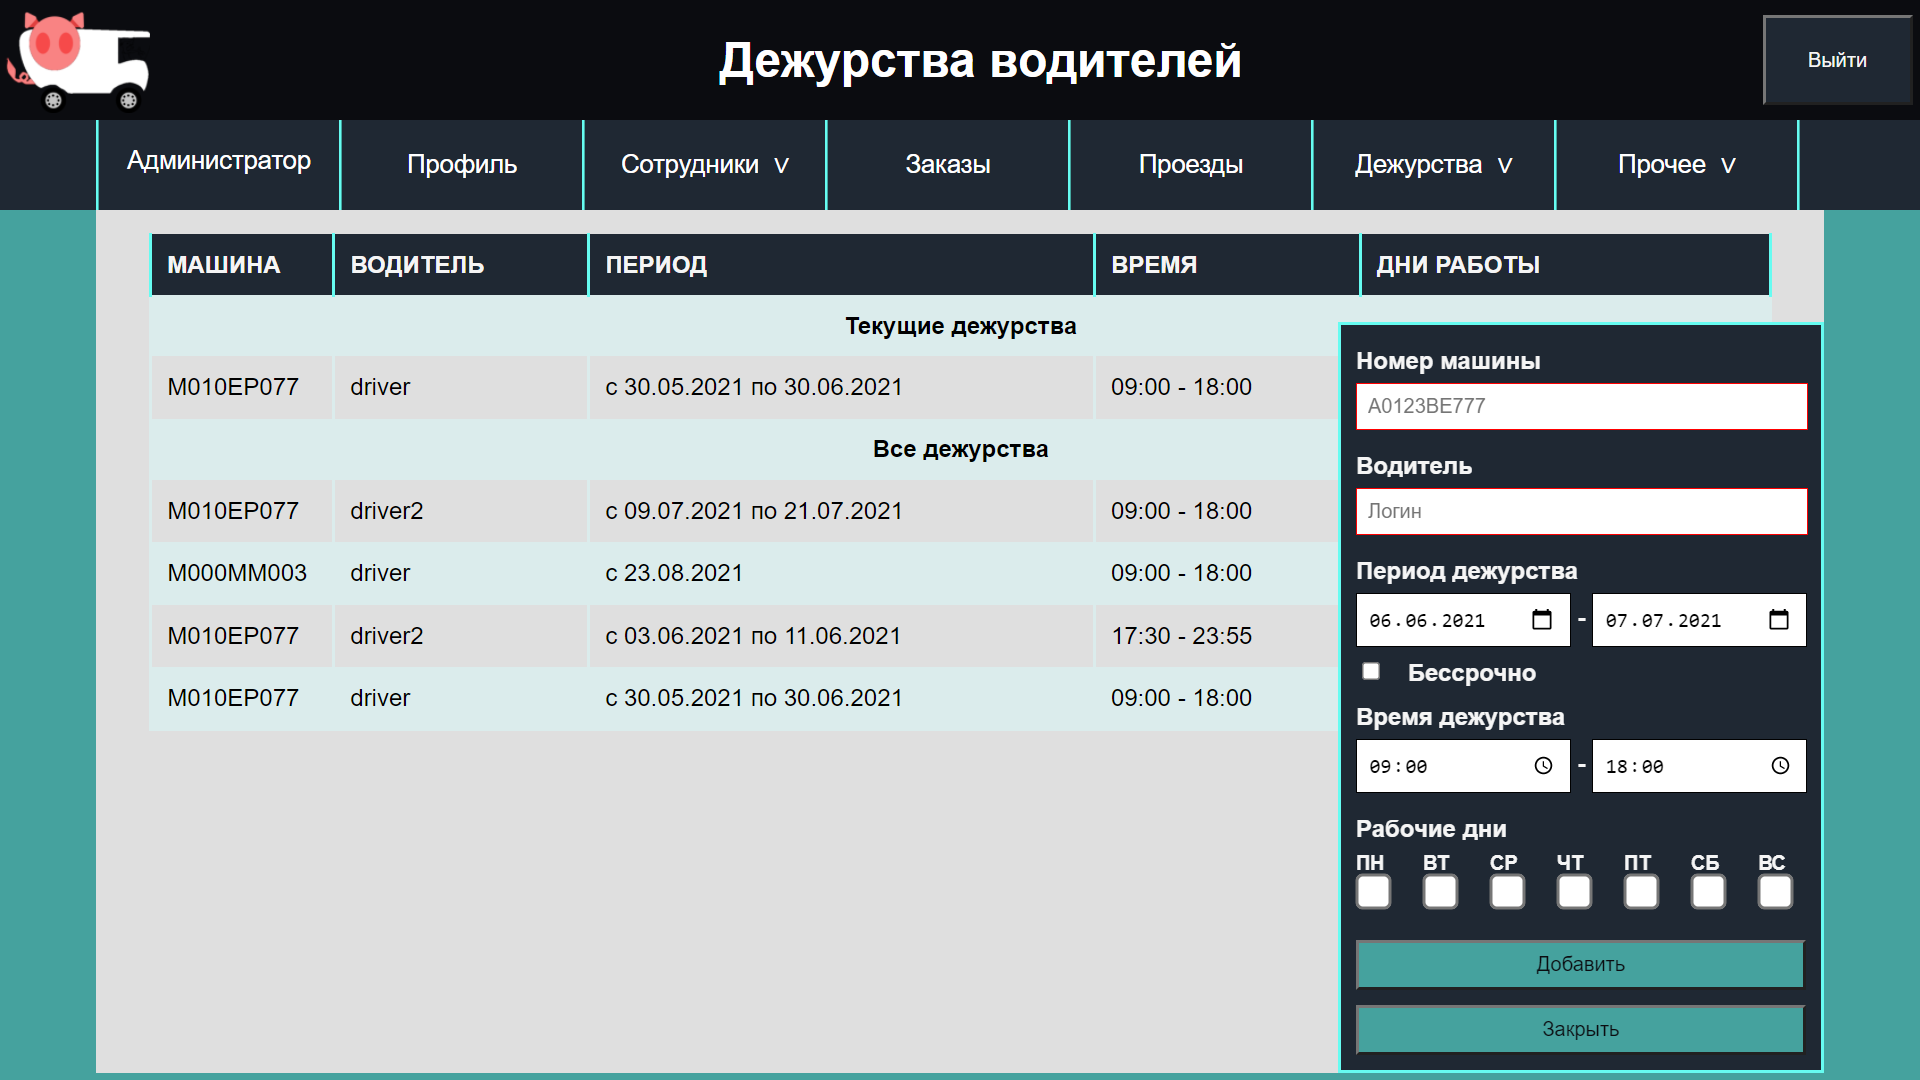
\includegraphics[scale=0.43, angle=0]{sc/driver_duty}}
		\caption{Страница просмотра и назначения дежурств водителей}
	\end{center}
\end{figure}

\begin{figure}[h!] \label{trucks_sc}
	\begin{center}
		%		{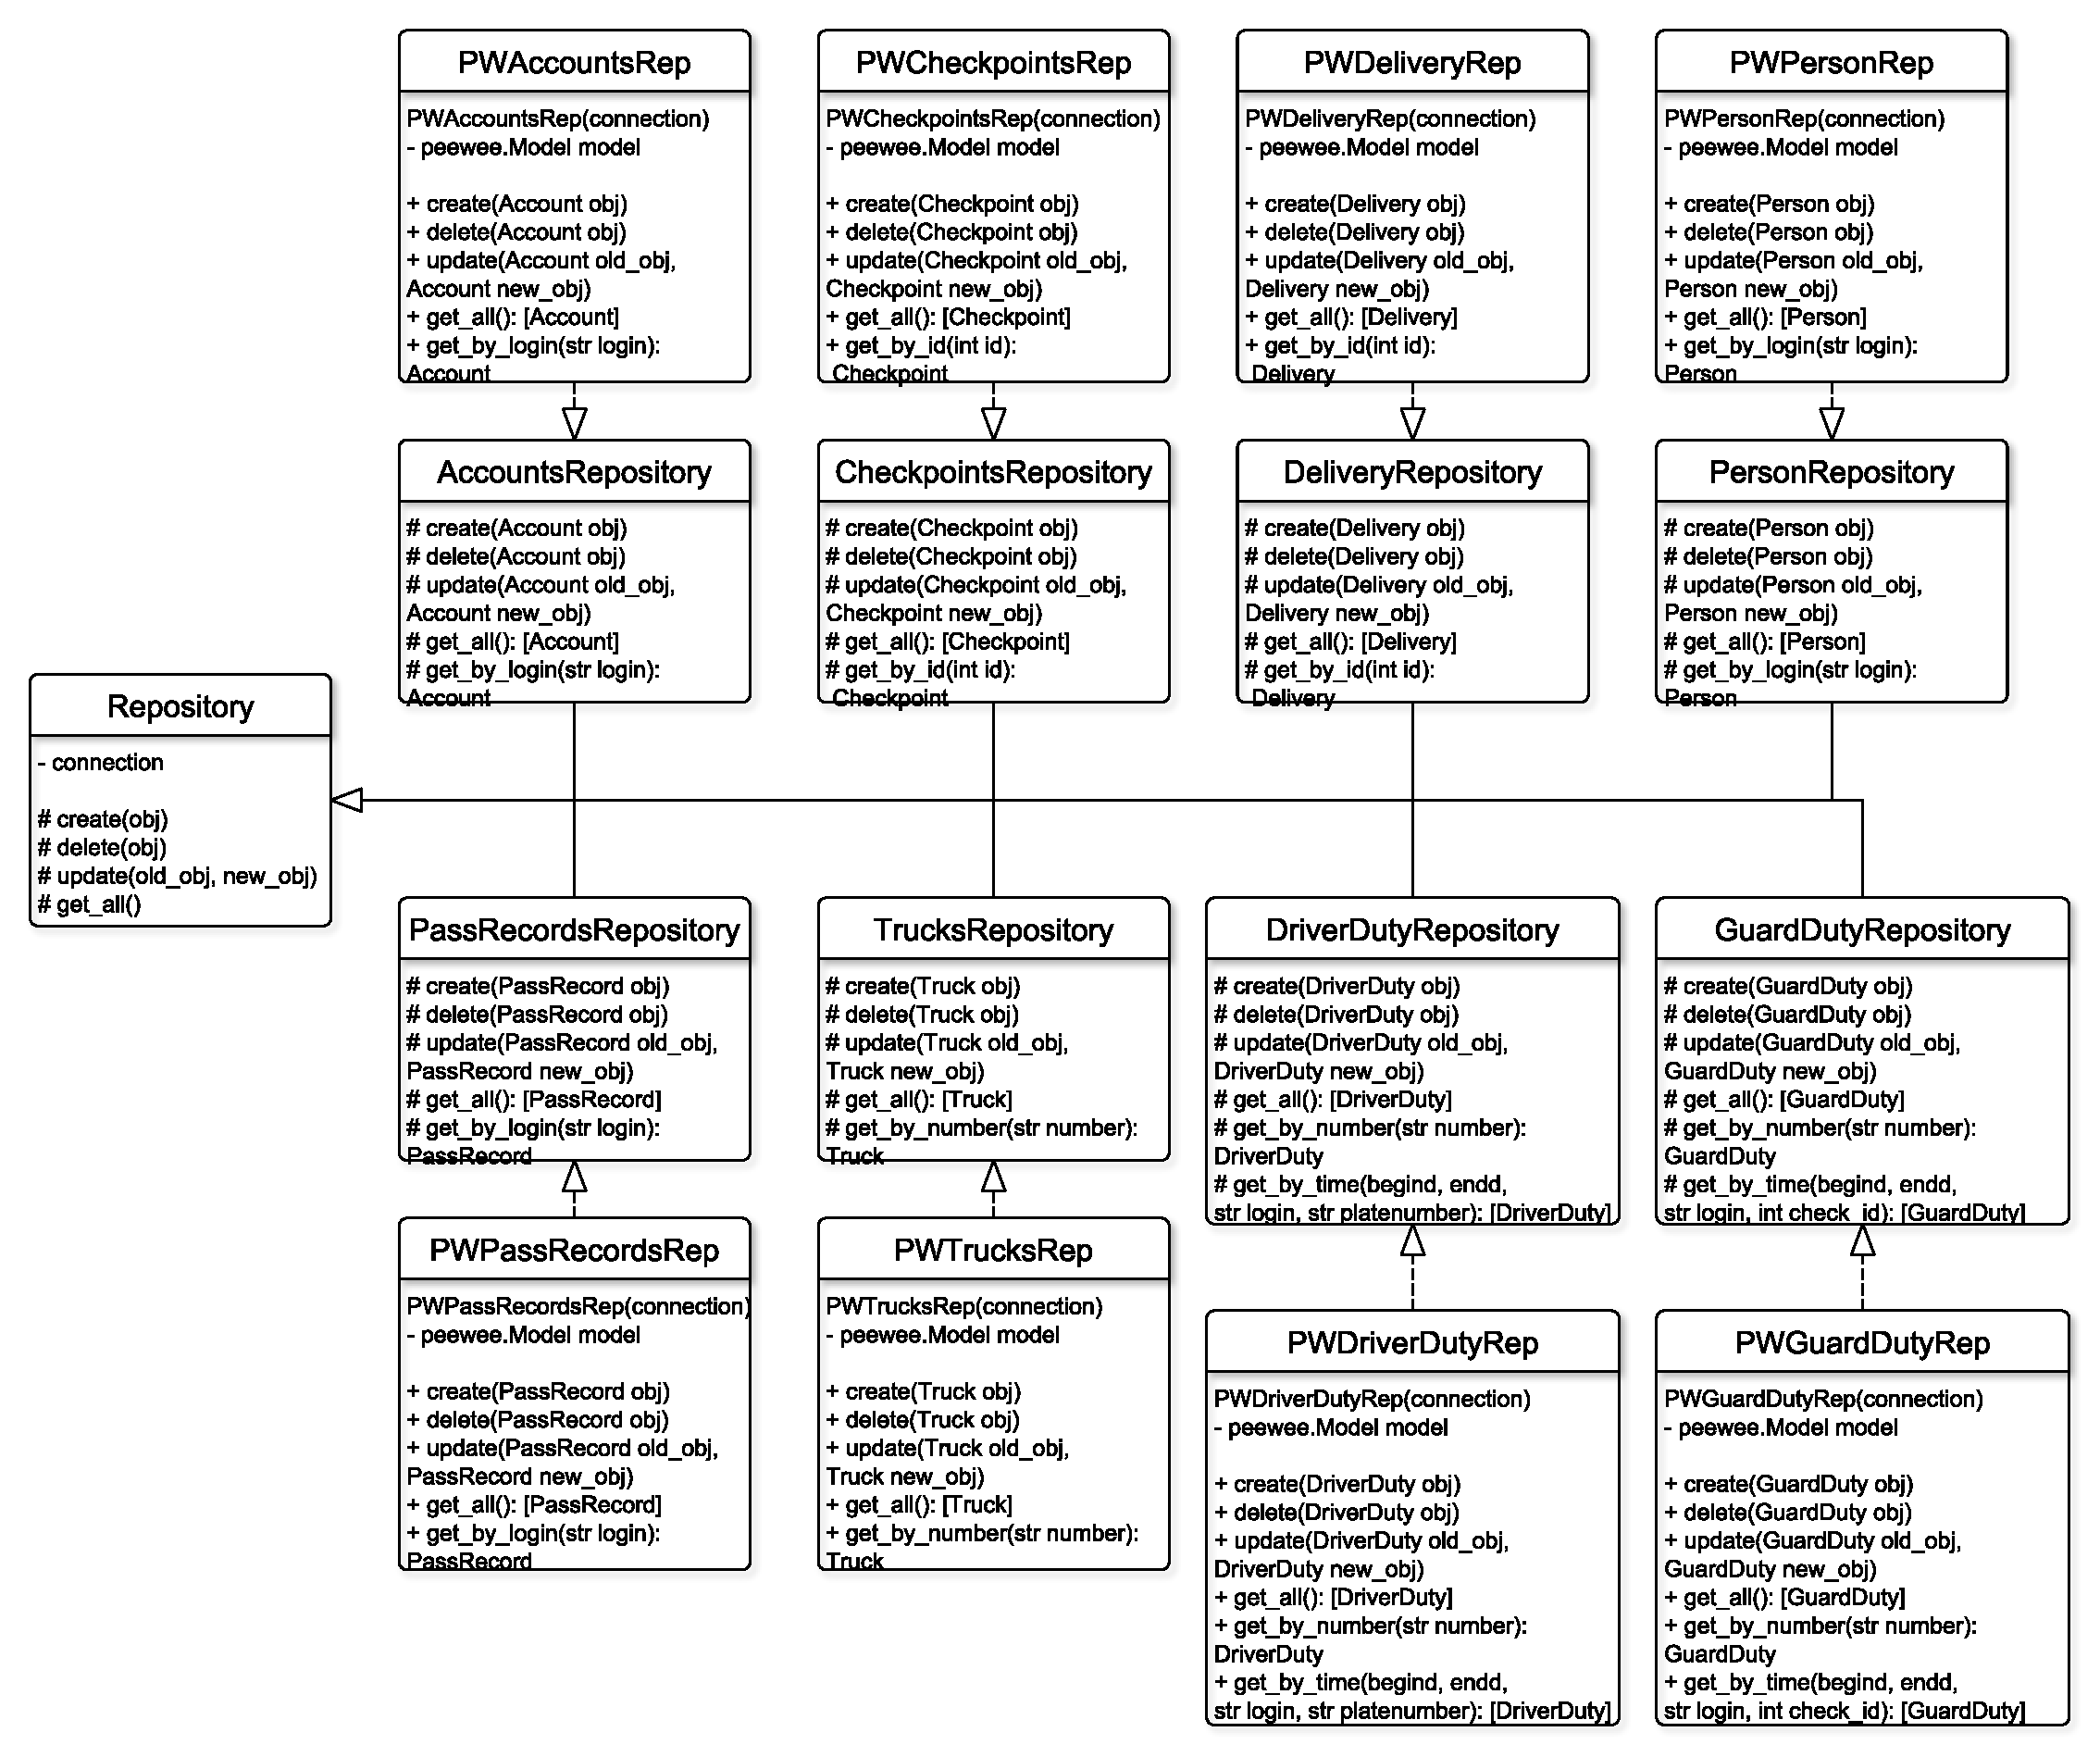
\includegraphics[height=14cm, width = 14cm]{uml/repsoitory.pdf}}
		{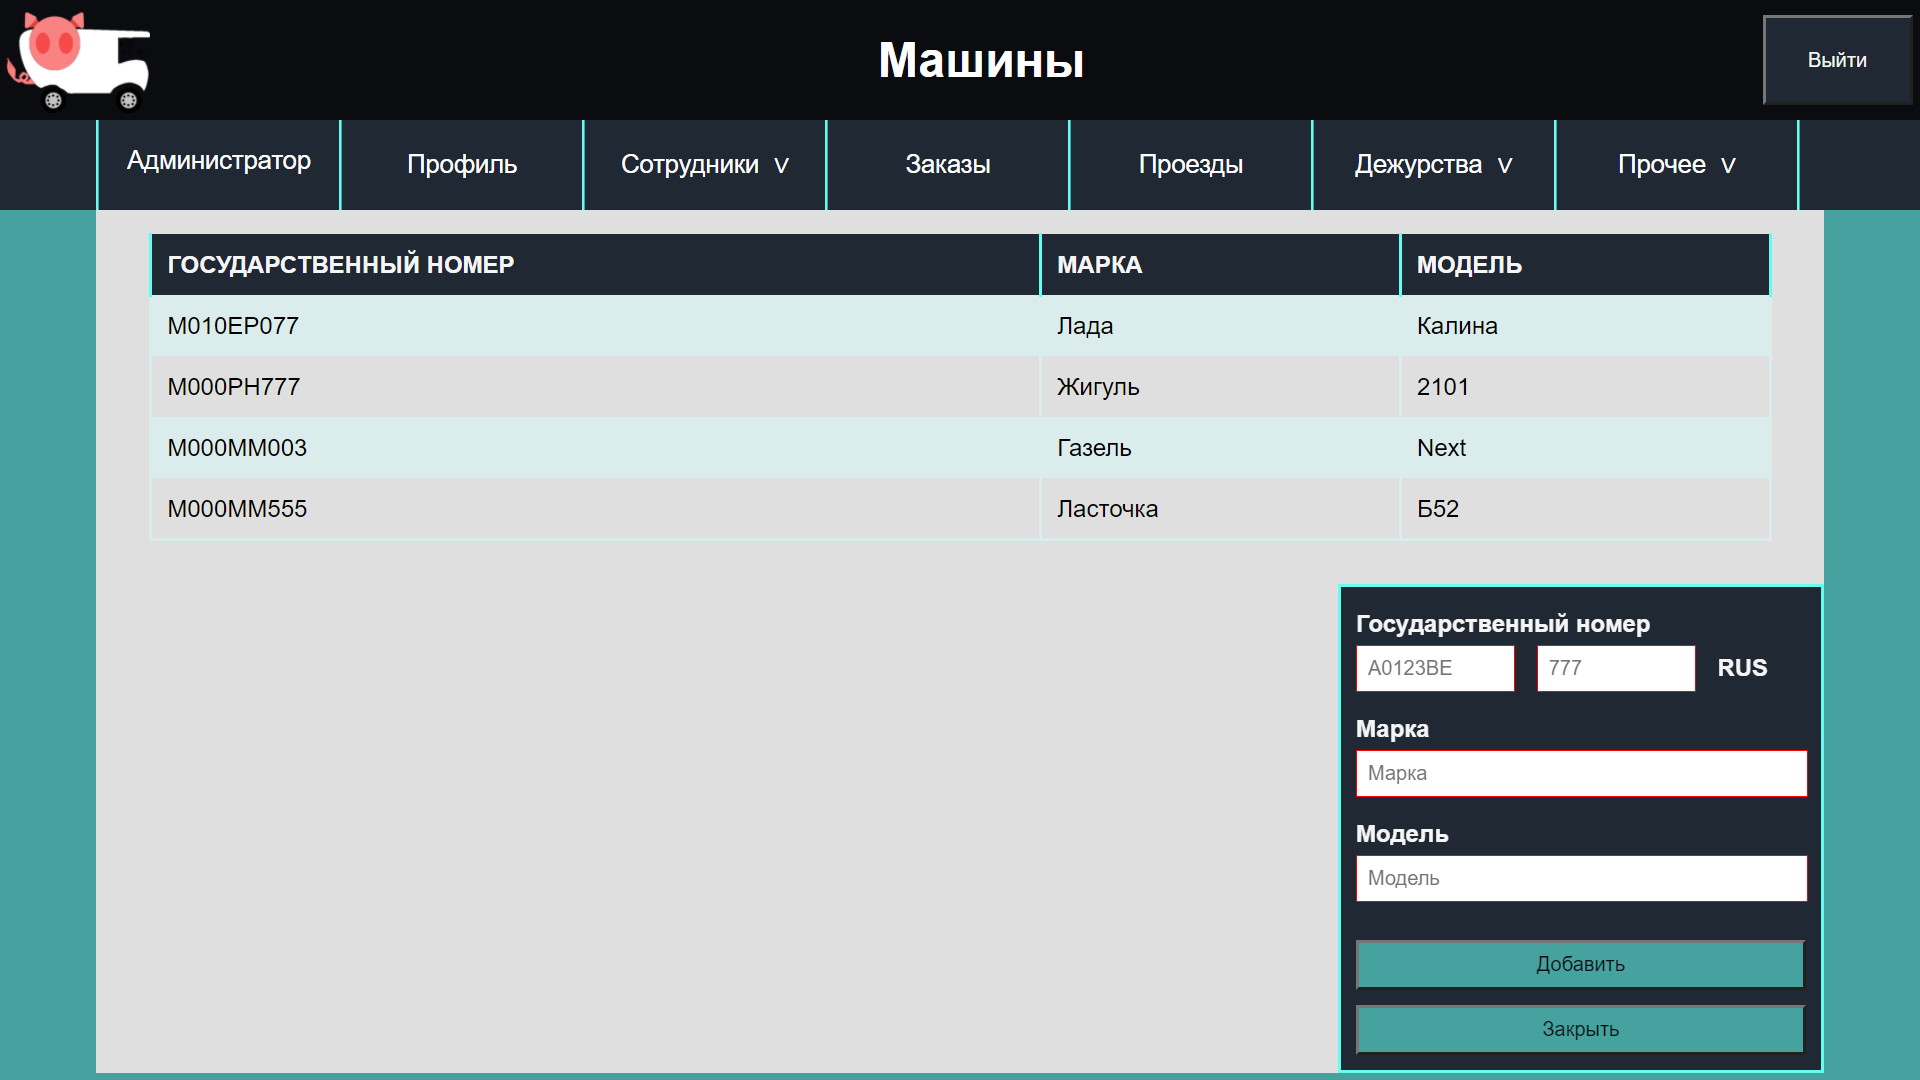
\includegraphics[scale=0.43, angle=0]{sc/trucks}}
		\caption{Страница просмотра и регистрации машин}
	\end{center}
\end{figure}

\begin{figure}[h!] \label{pick_delivery_sc}
	\begin{center}
		%		{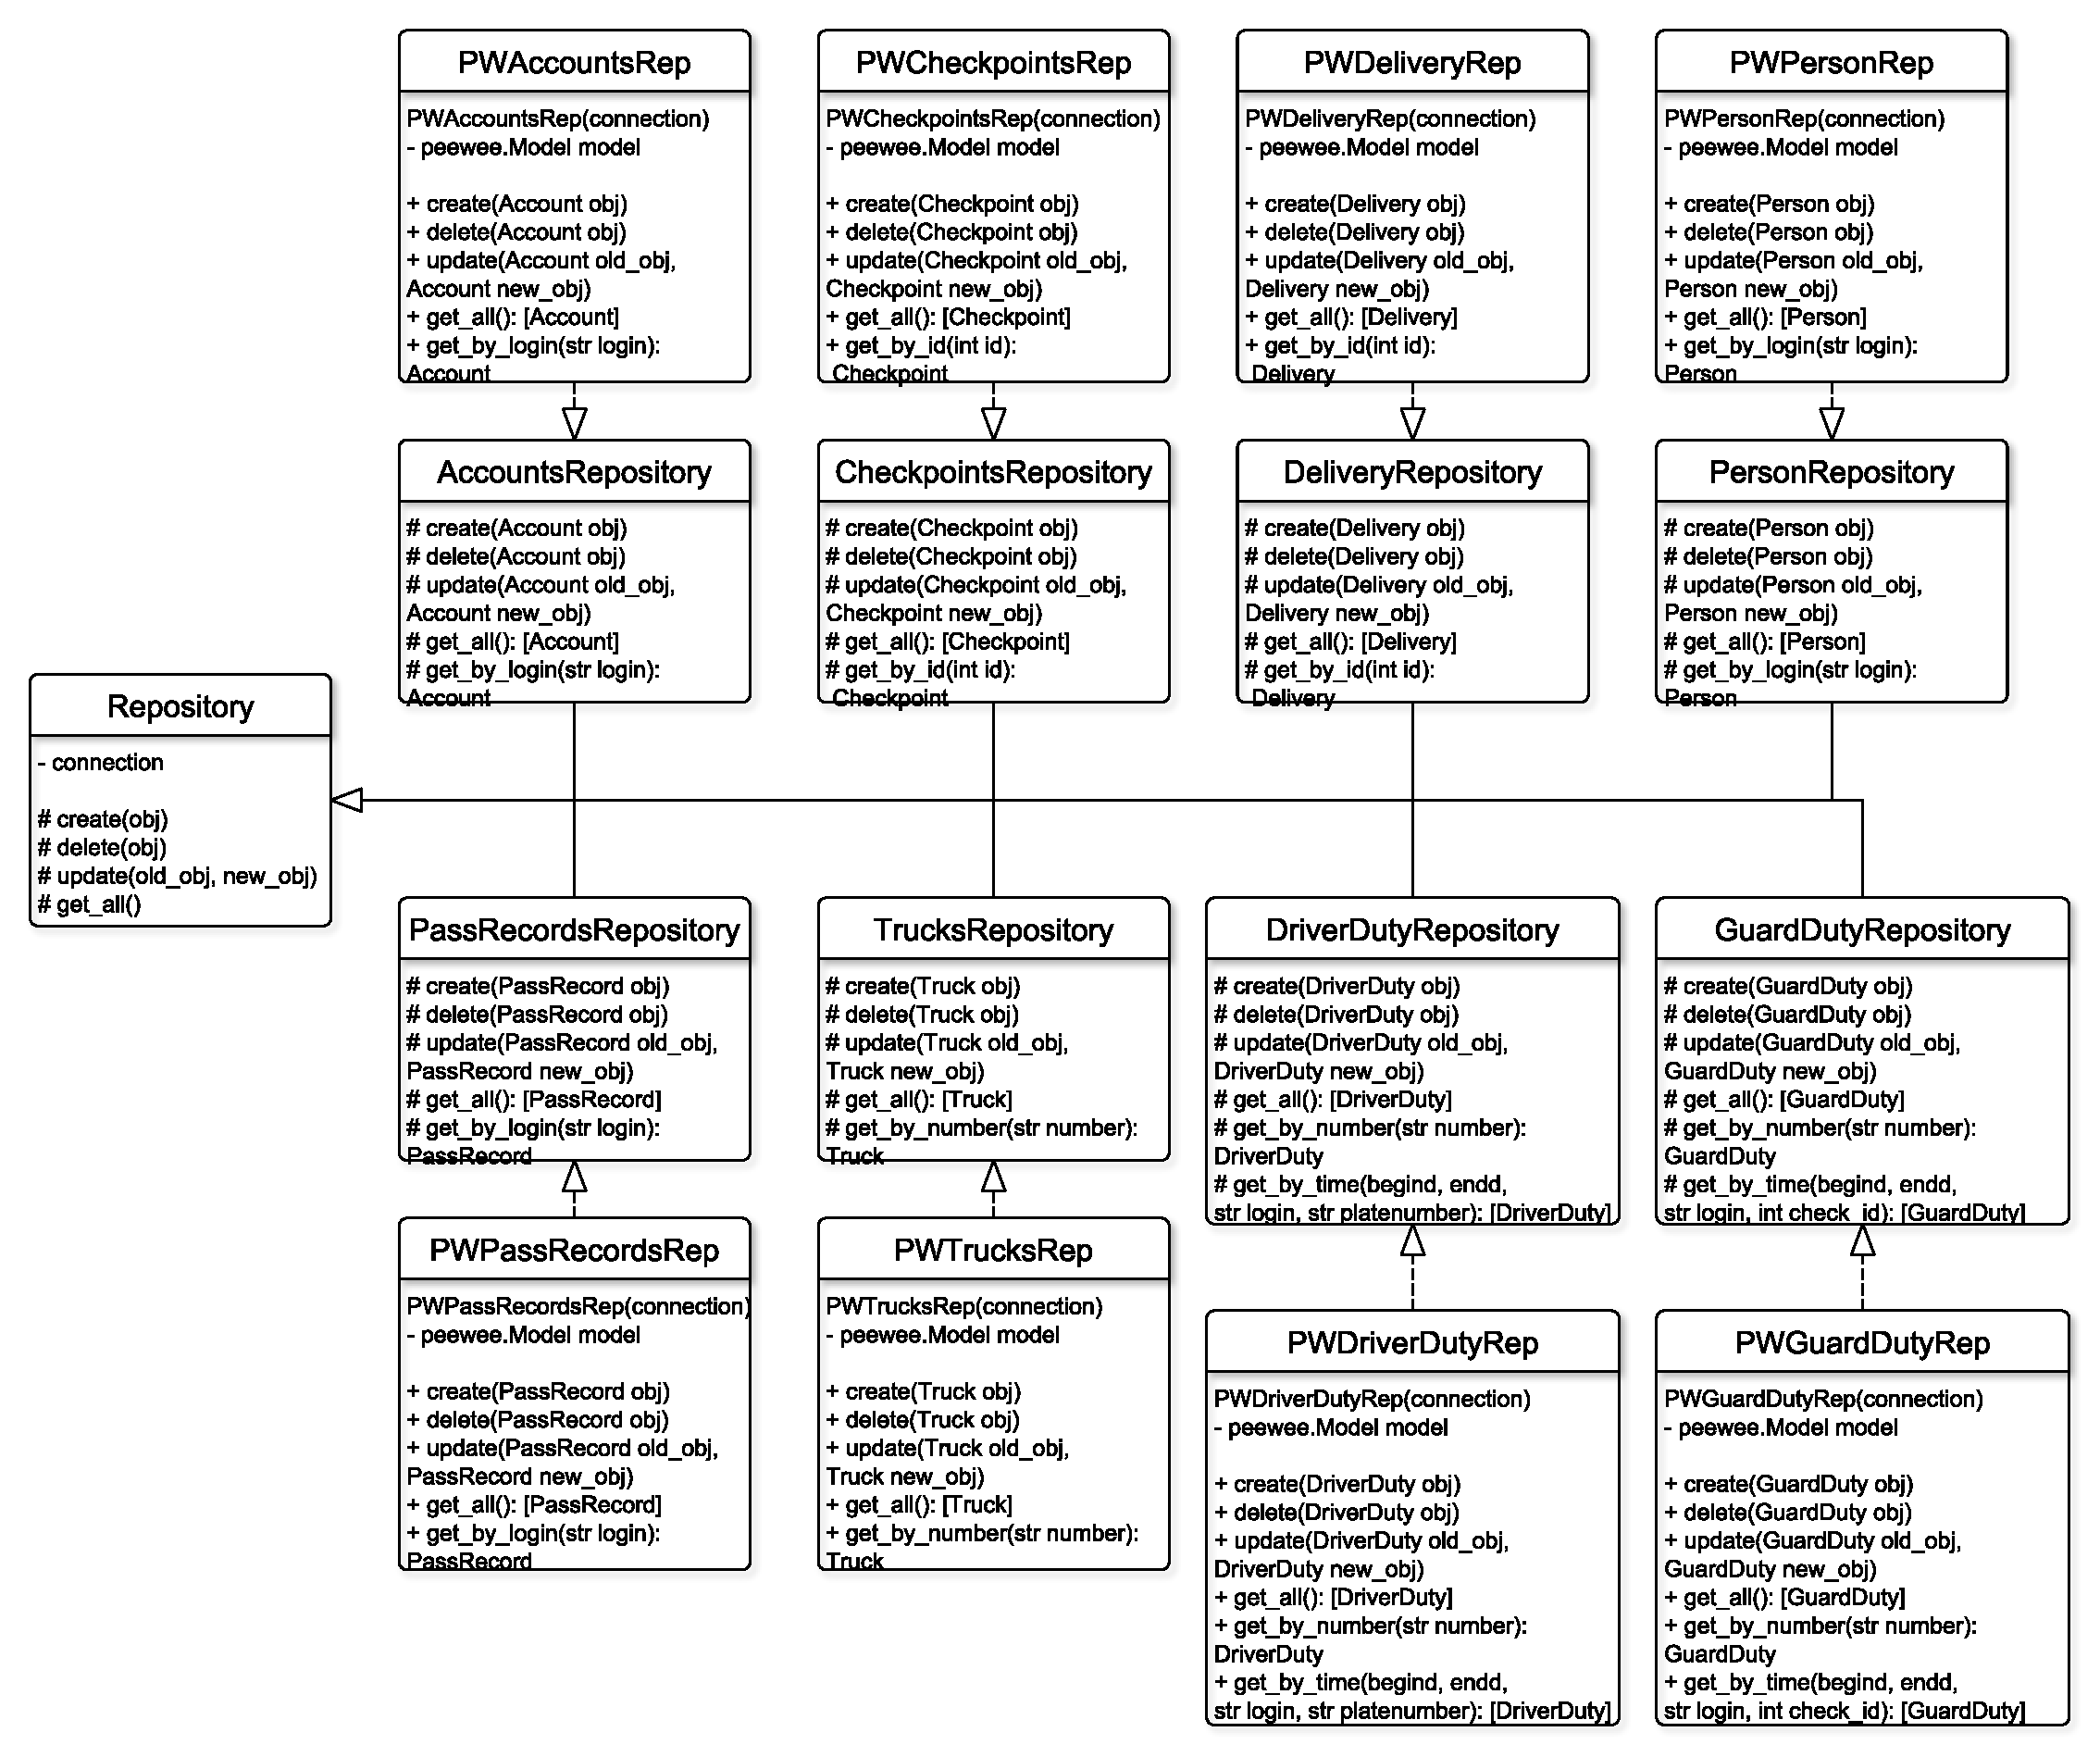
\includegraphics[height=14cm, width = 14cm]{uml/repsoitory.pdf}}
		{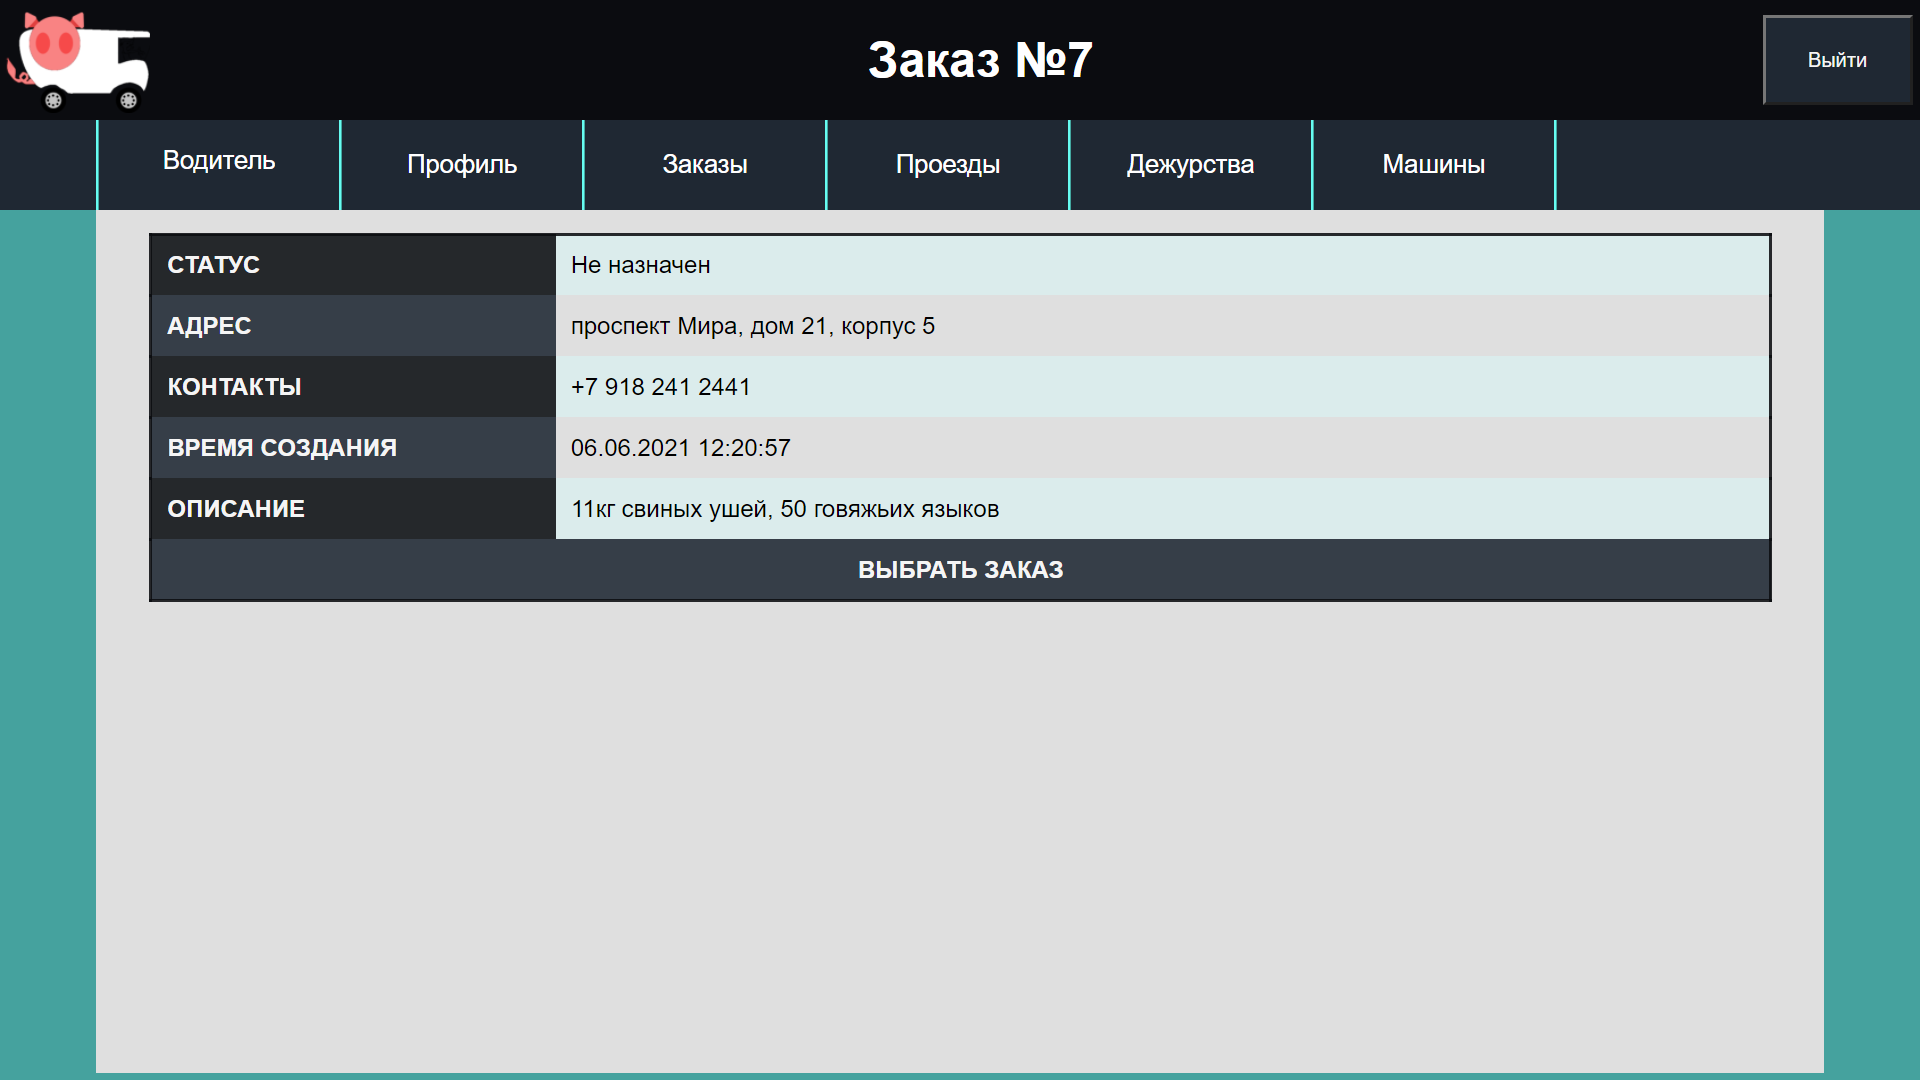
\includegraphics[scale=0.4, angle=0]{sc/pick_delivery}}
		\caption{Страница просмотра и выбора заказа (для роли водителя)}
	\end{center}
\end{figure}

\begin{figure}[h!] \label{driver_profile_sc}
	\begin{center}
		%		{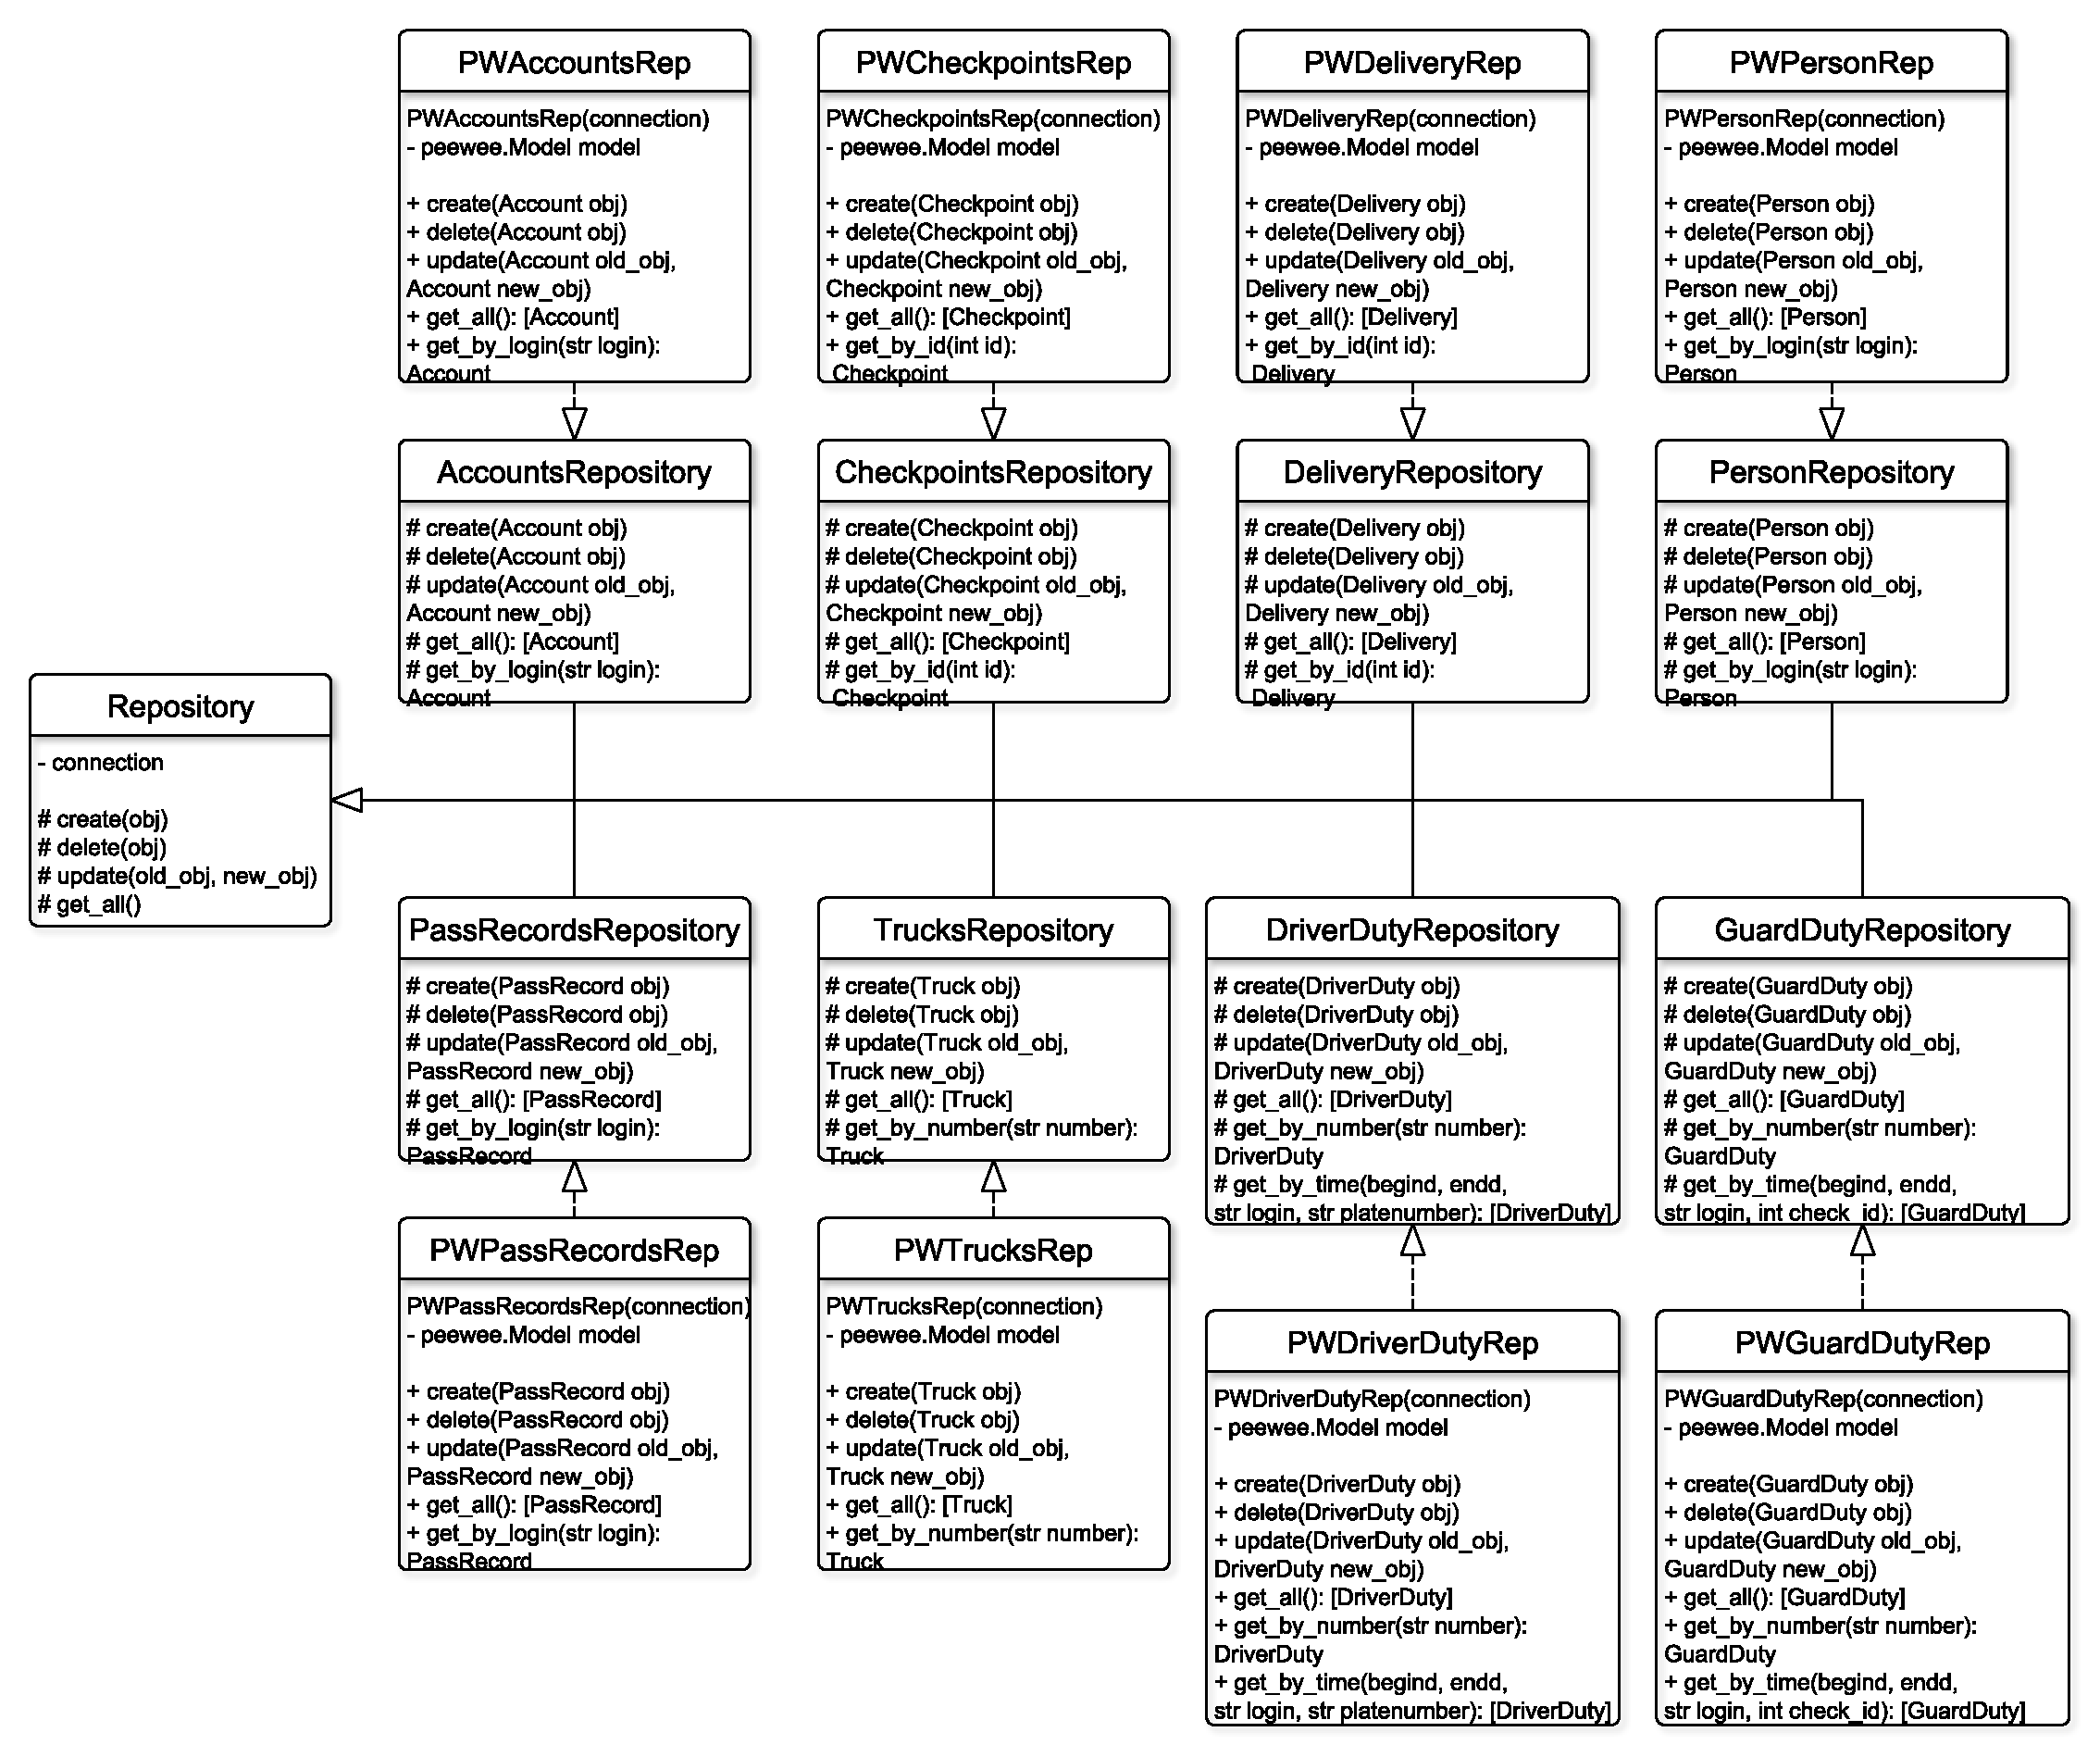
\includegraphics[height=14cm, width = 14cm]{uml/repsoitory.pdf}}
		{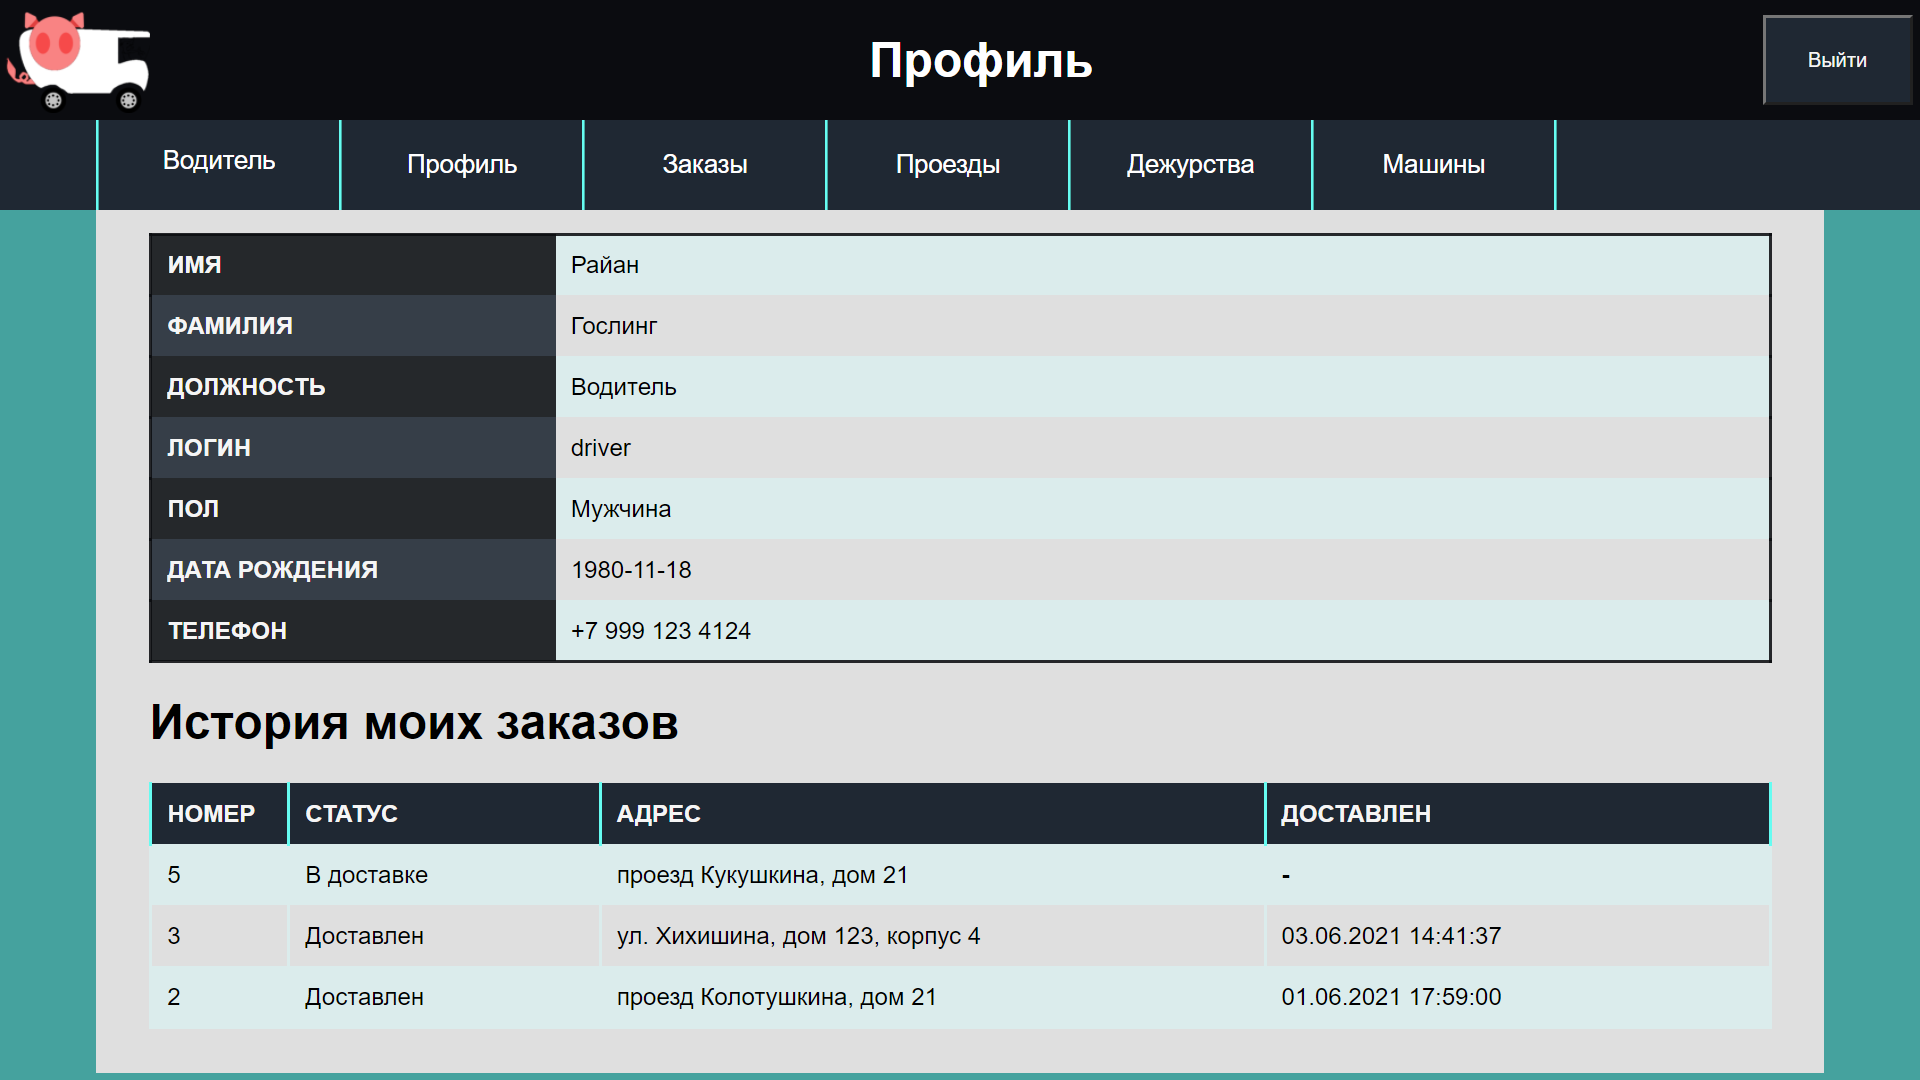
\includegraphics[scale=0.4, angle=0]{sc/driver_profile}}
		\caption{Личная страница (для роли водителя)}
	\end{center}
\end{figure}

\begin{figure}[h!] \label{guard_duty_sc}
	\begin{center}
		%		{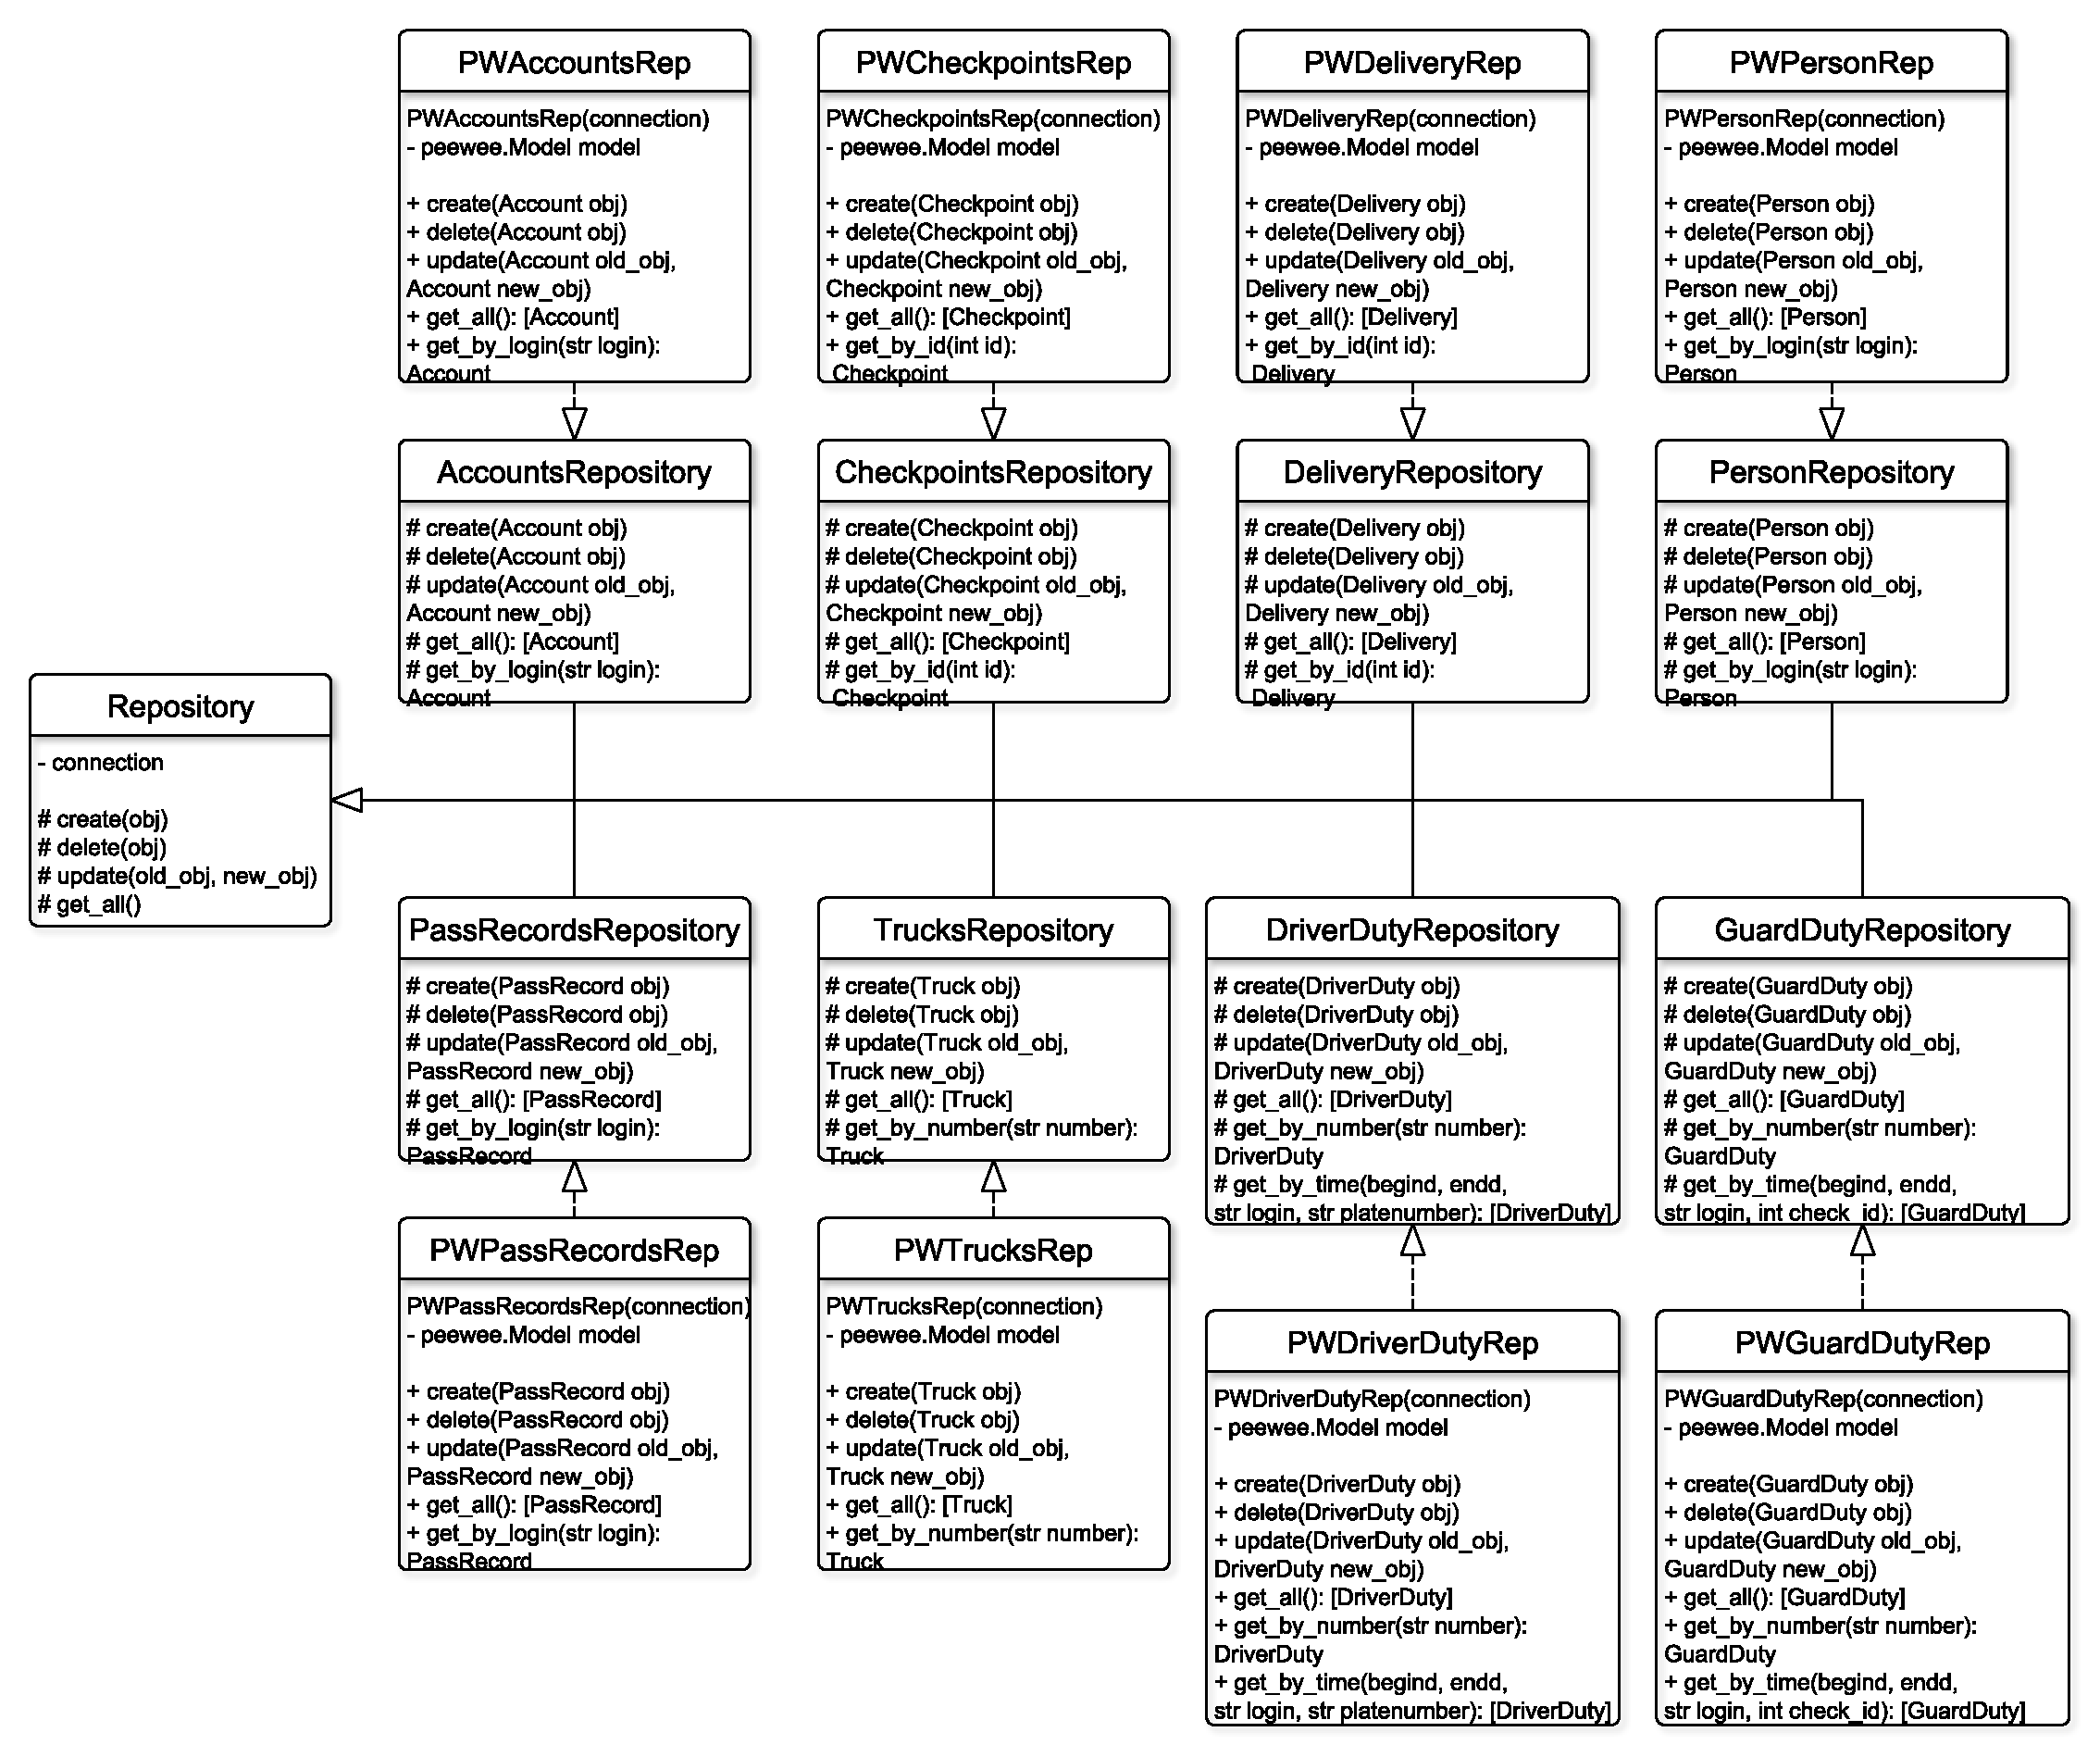
\includegraphics[height=14cm, width = 14cm]{uml/repsoitory.pdf}}
		{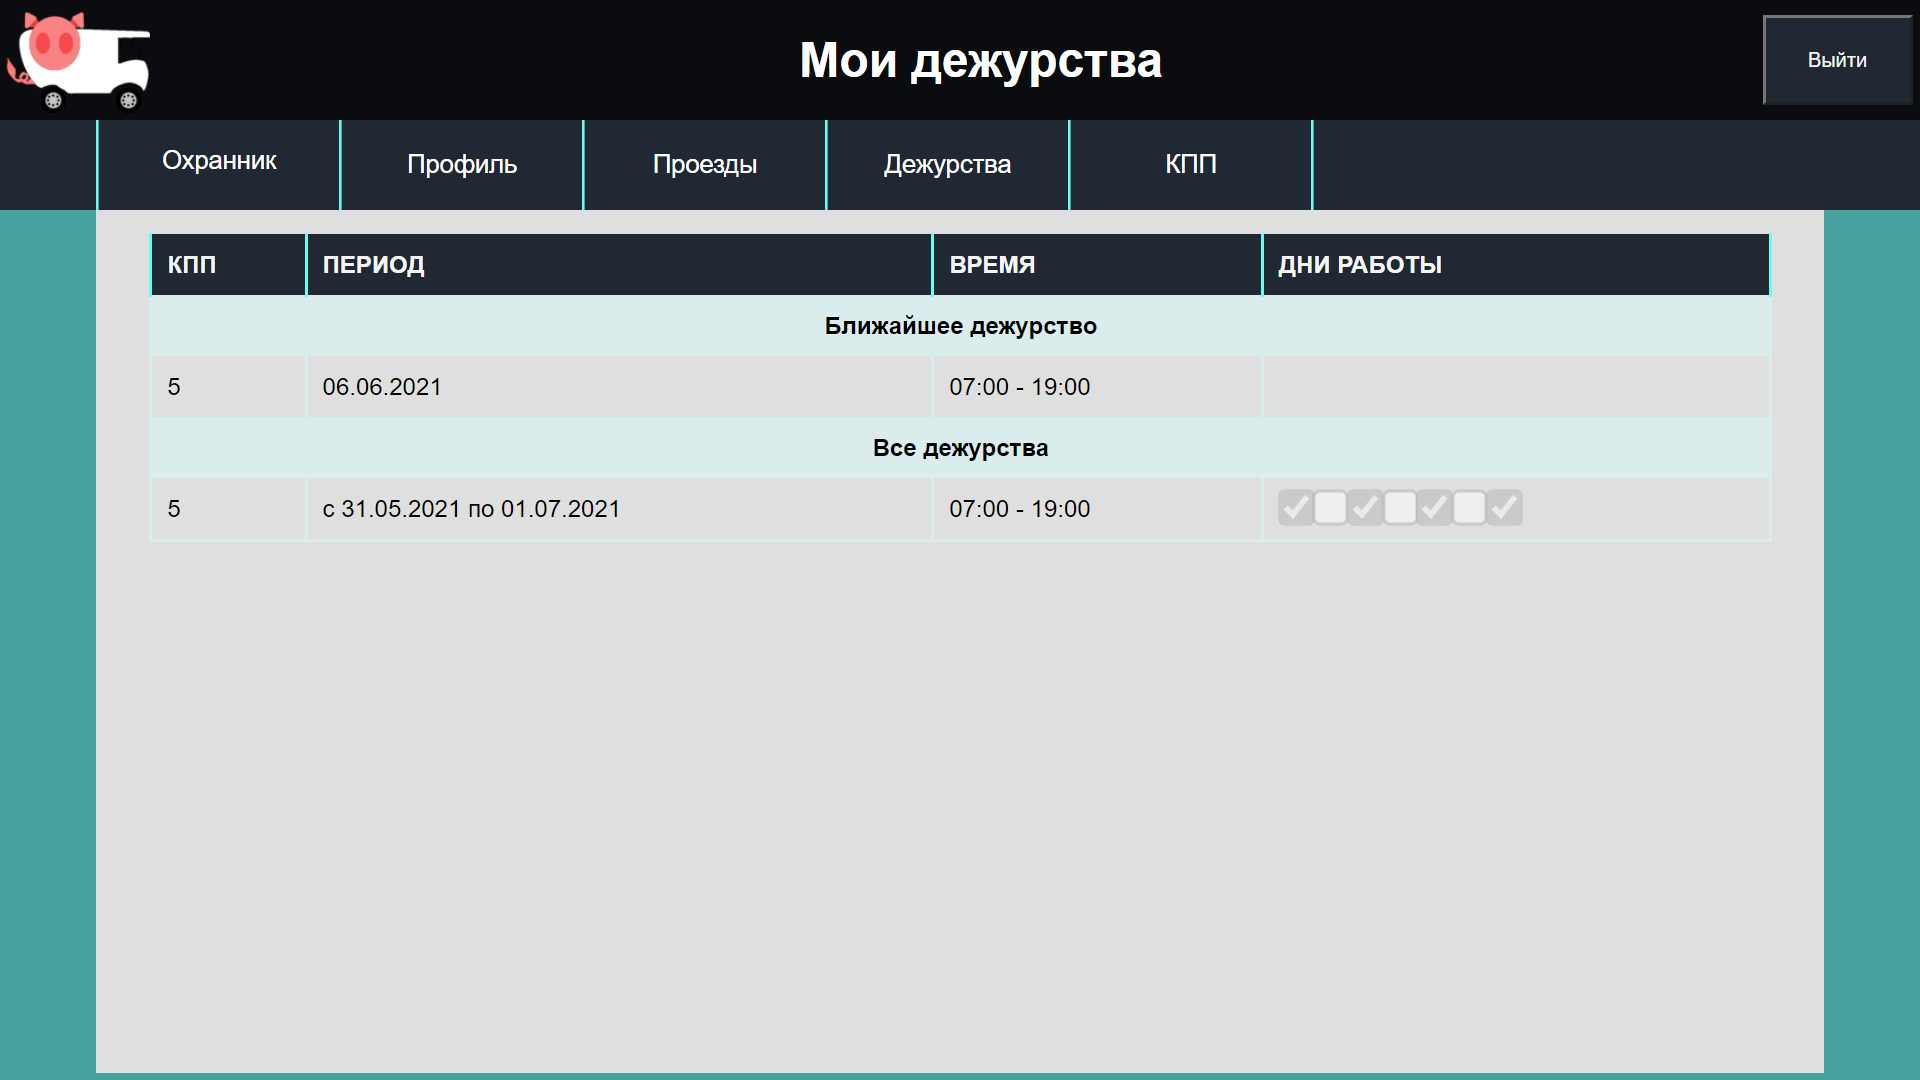
\includegraphics[scale=0.4, angle=0]{sc/guard_duty}}
		\caption{Страница просмотра дежурств (для роли охранника)}
	\end{center}
\end{figure}

\begin{figure}[h!] \label{pass_guard_sc}
	\begin{center}
		%		{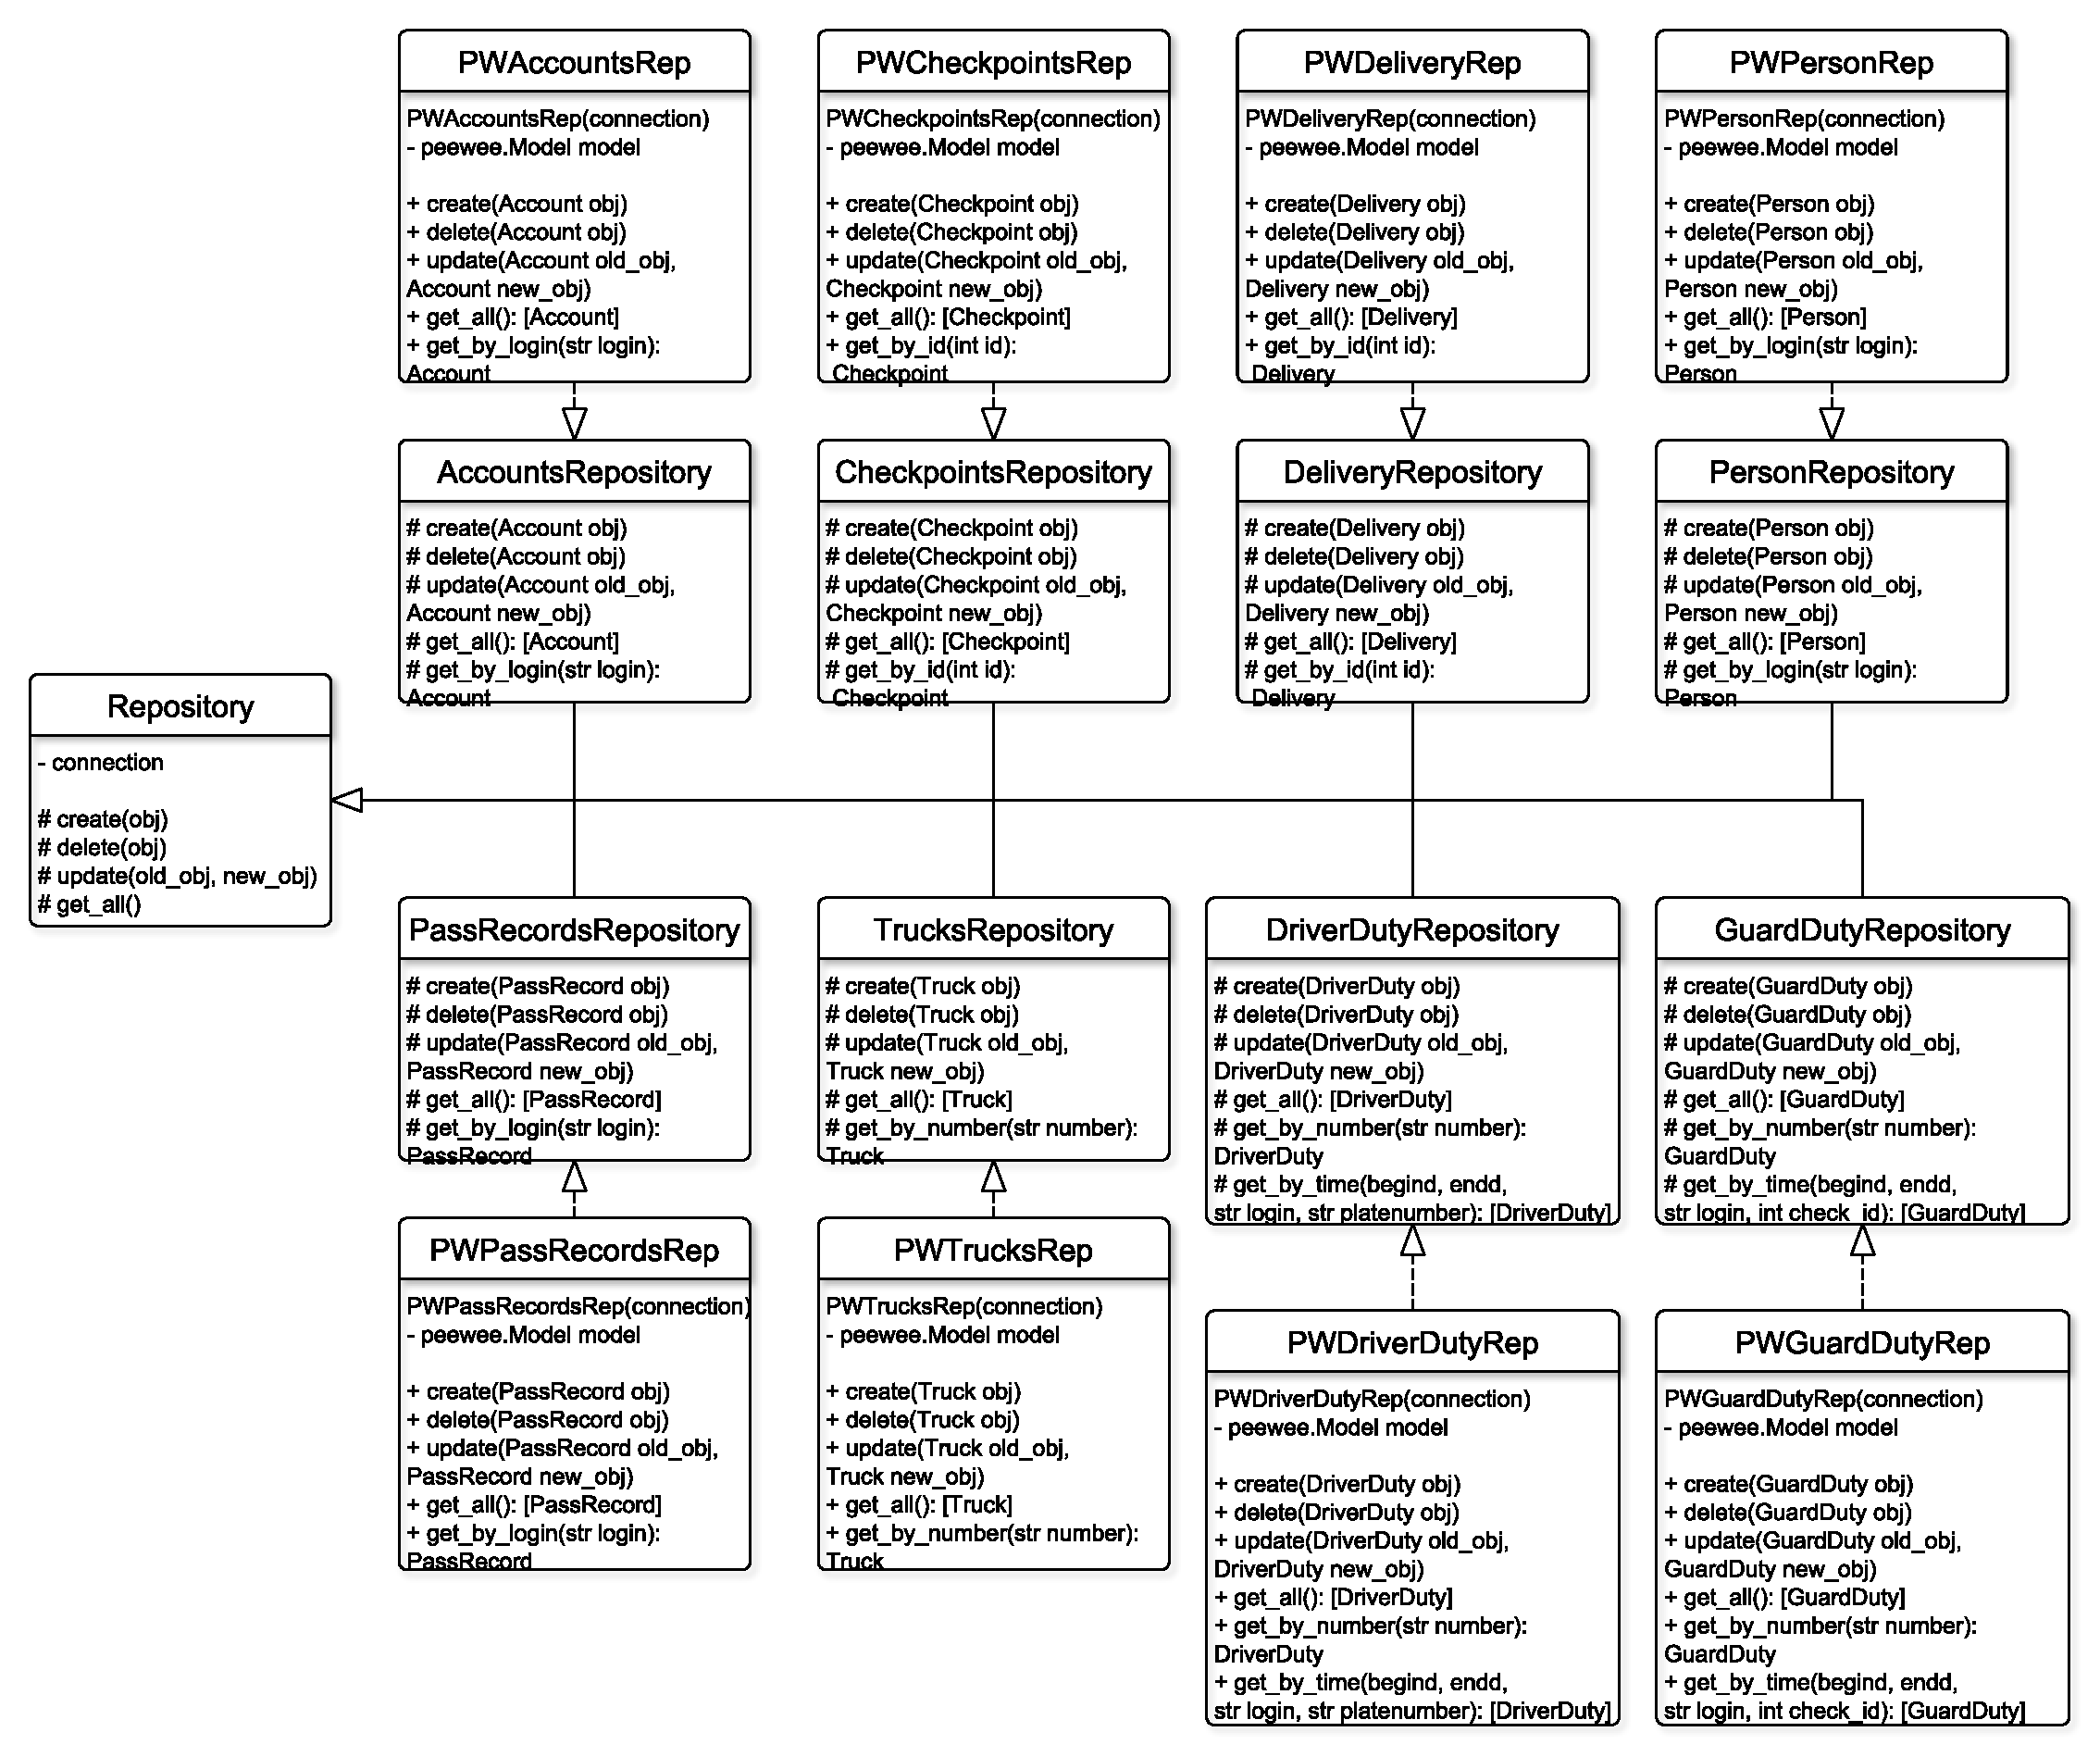
\includegraphics[height=14cm, width = 14cm]{uml/repsoitory.pdf}}
		{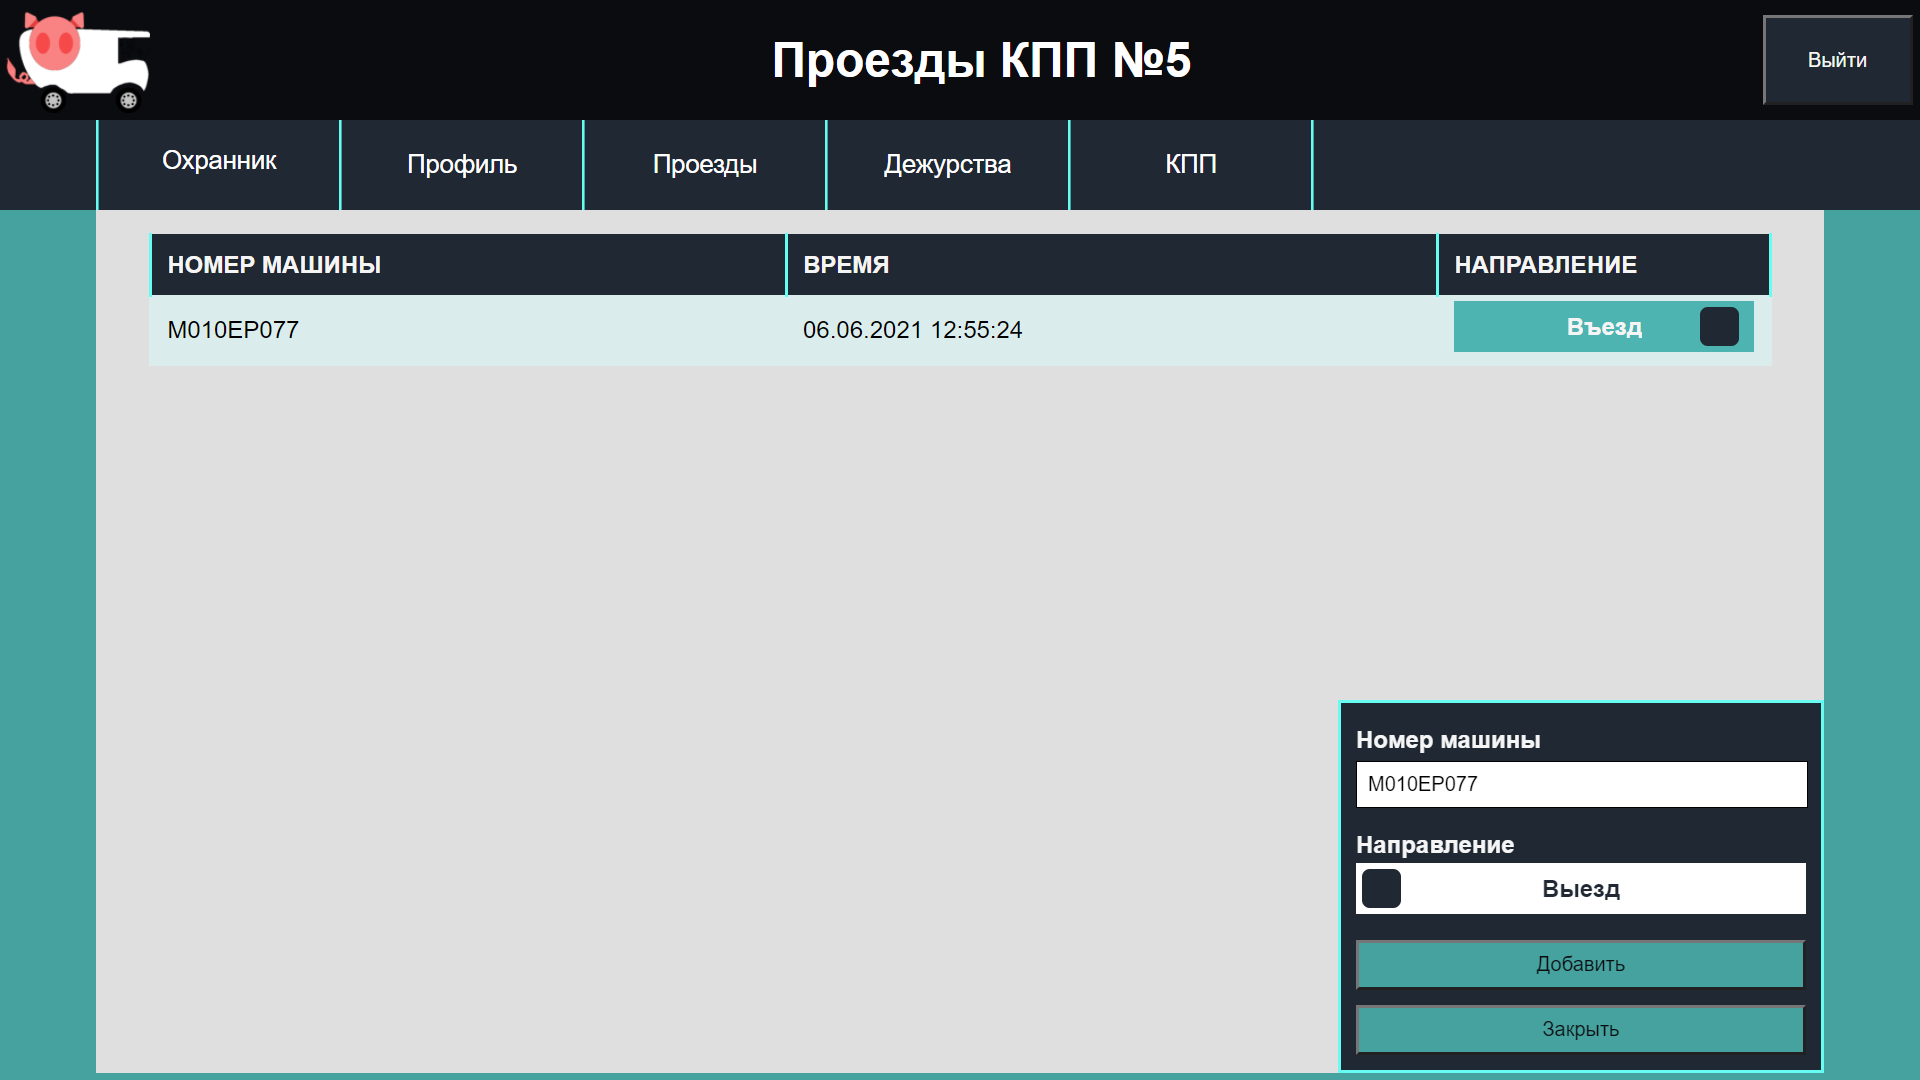
\includegraphics[scale=0.4, angle=0]{sc/pass_guard}}
		\caption{Страница просмотра и добавления записей проездов (для роли охранника)}
	\end{center}
\end{figure}

\newpage
Для неавторизованного пользователя доступны страницы входа в аккаунт и регистрации (рисунок \hyperref[login_sc]{3.16} и \hyperref[signup_sc]{3.17}) 

\begin{figure}[h!] \label{login_sc}
	\begin{center}
		%		{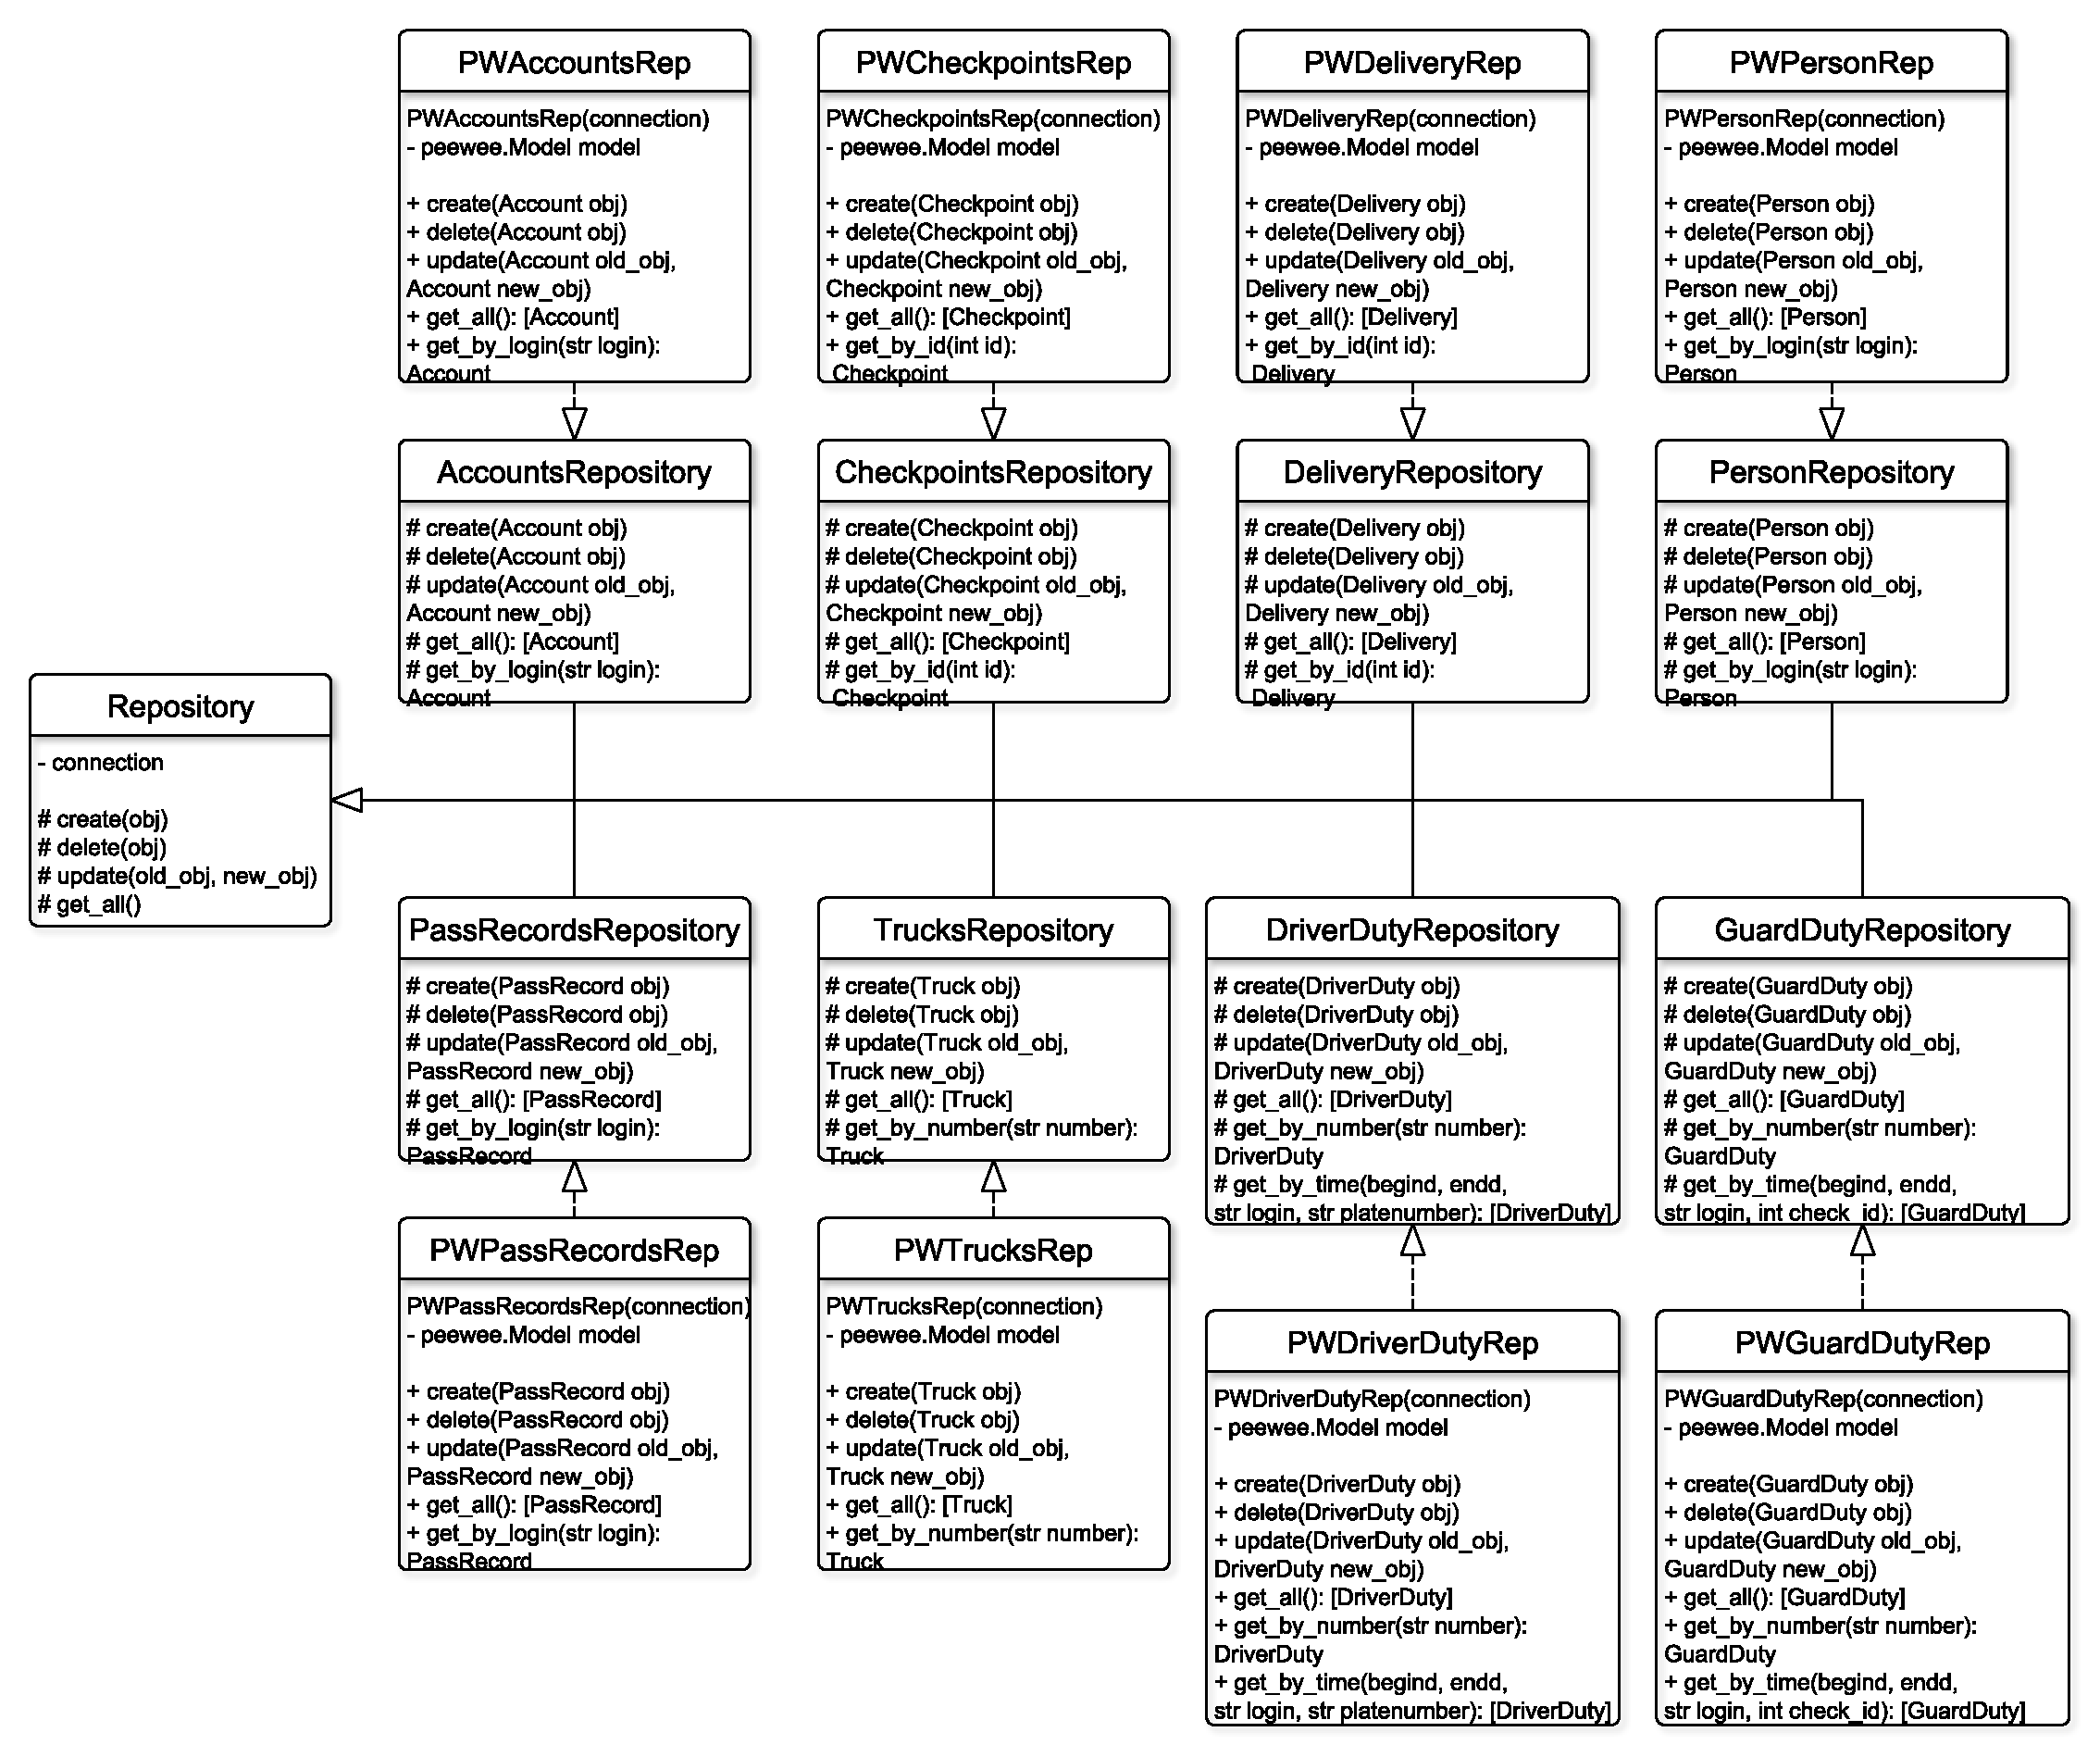
\includegraphics[height=14cm, width = 14cm]{uml/repsoitory.pdf}}
		{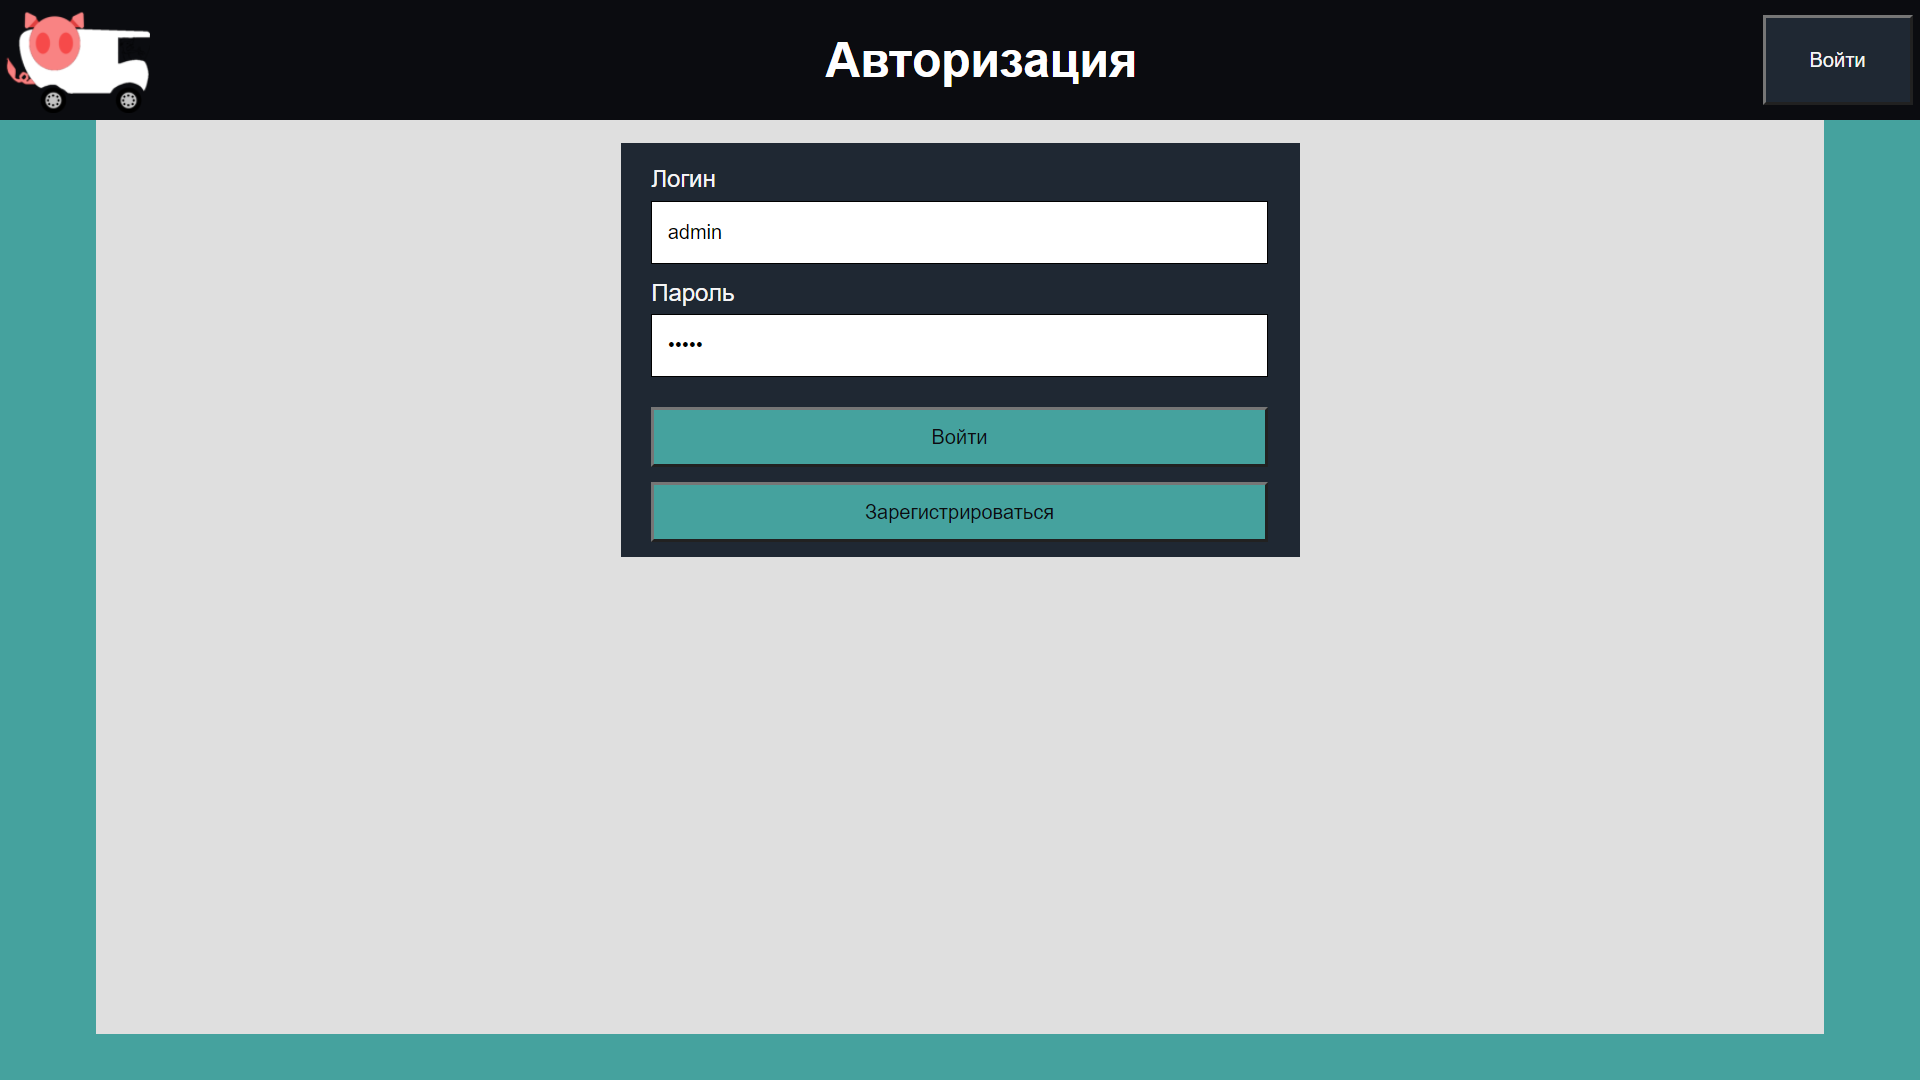
\includegraphics[scale=0.38, angle=0]{sc/login}}
		\caption{Страница авторизации}
	\end{center}
\end{figure}

\begin{figure}[h!] \label{signup_sc}
	\begin{center}
		%		{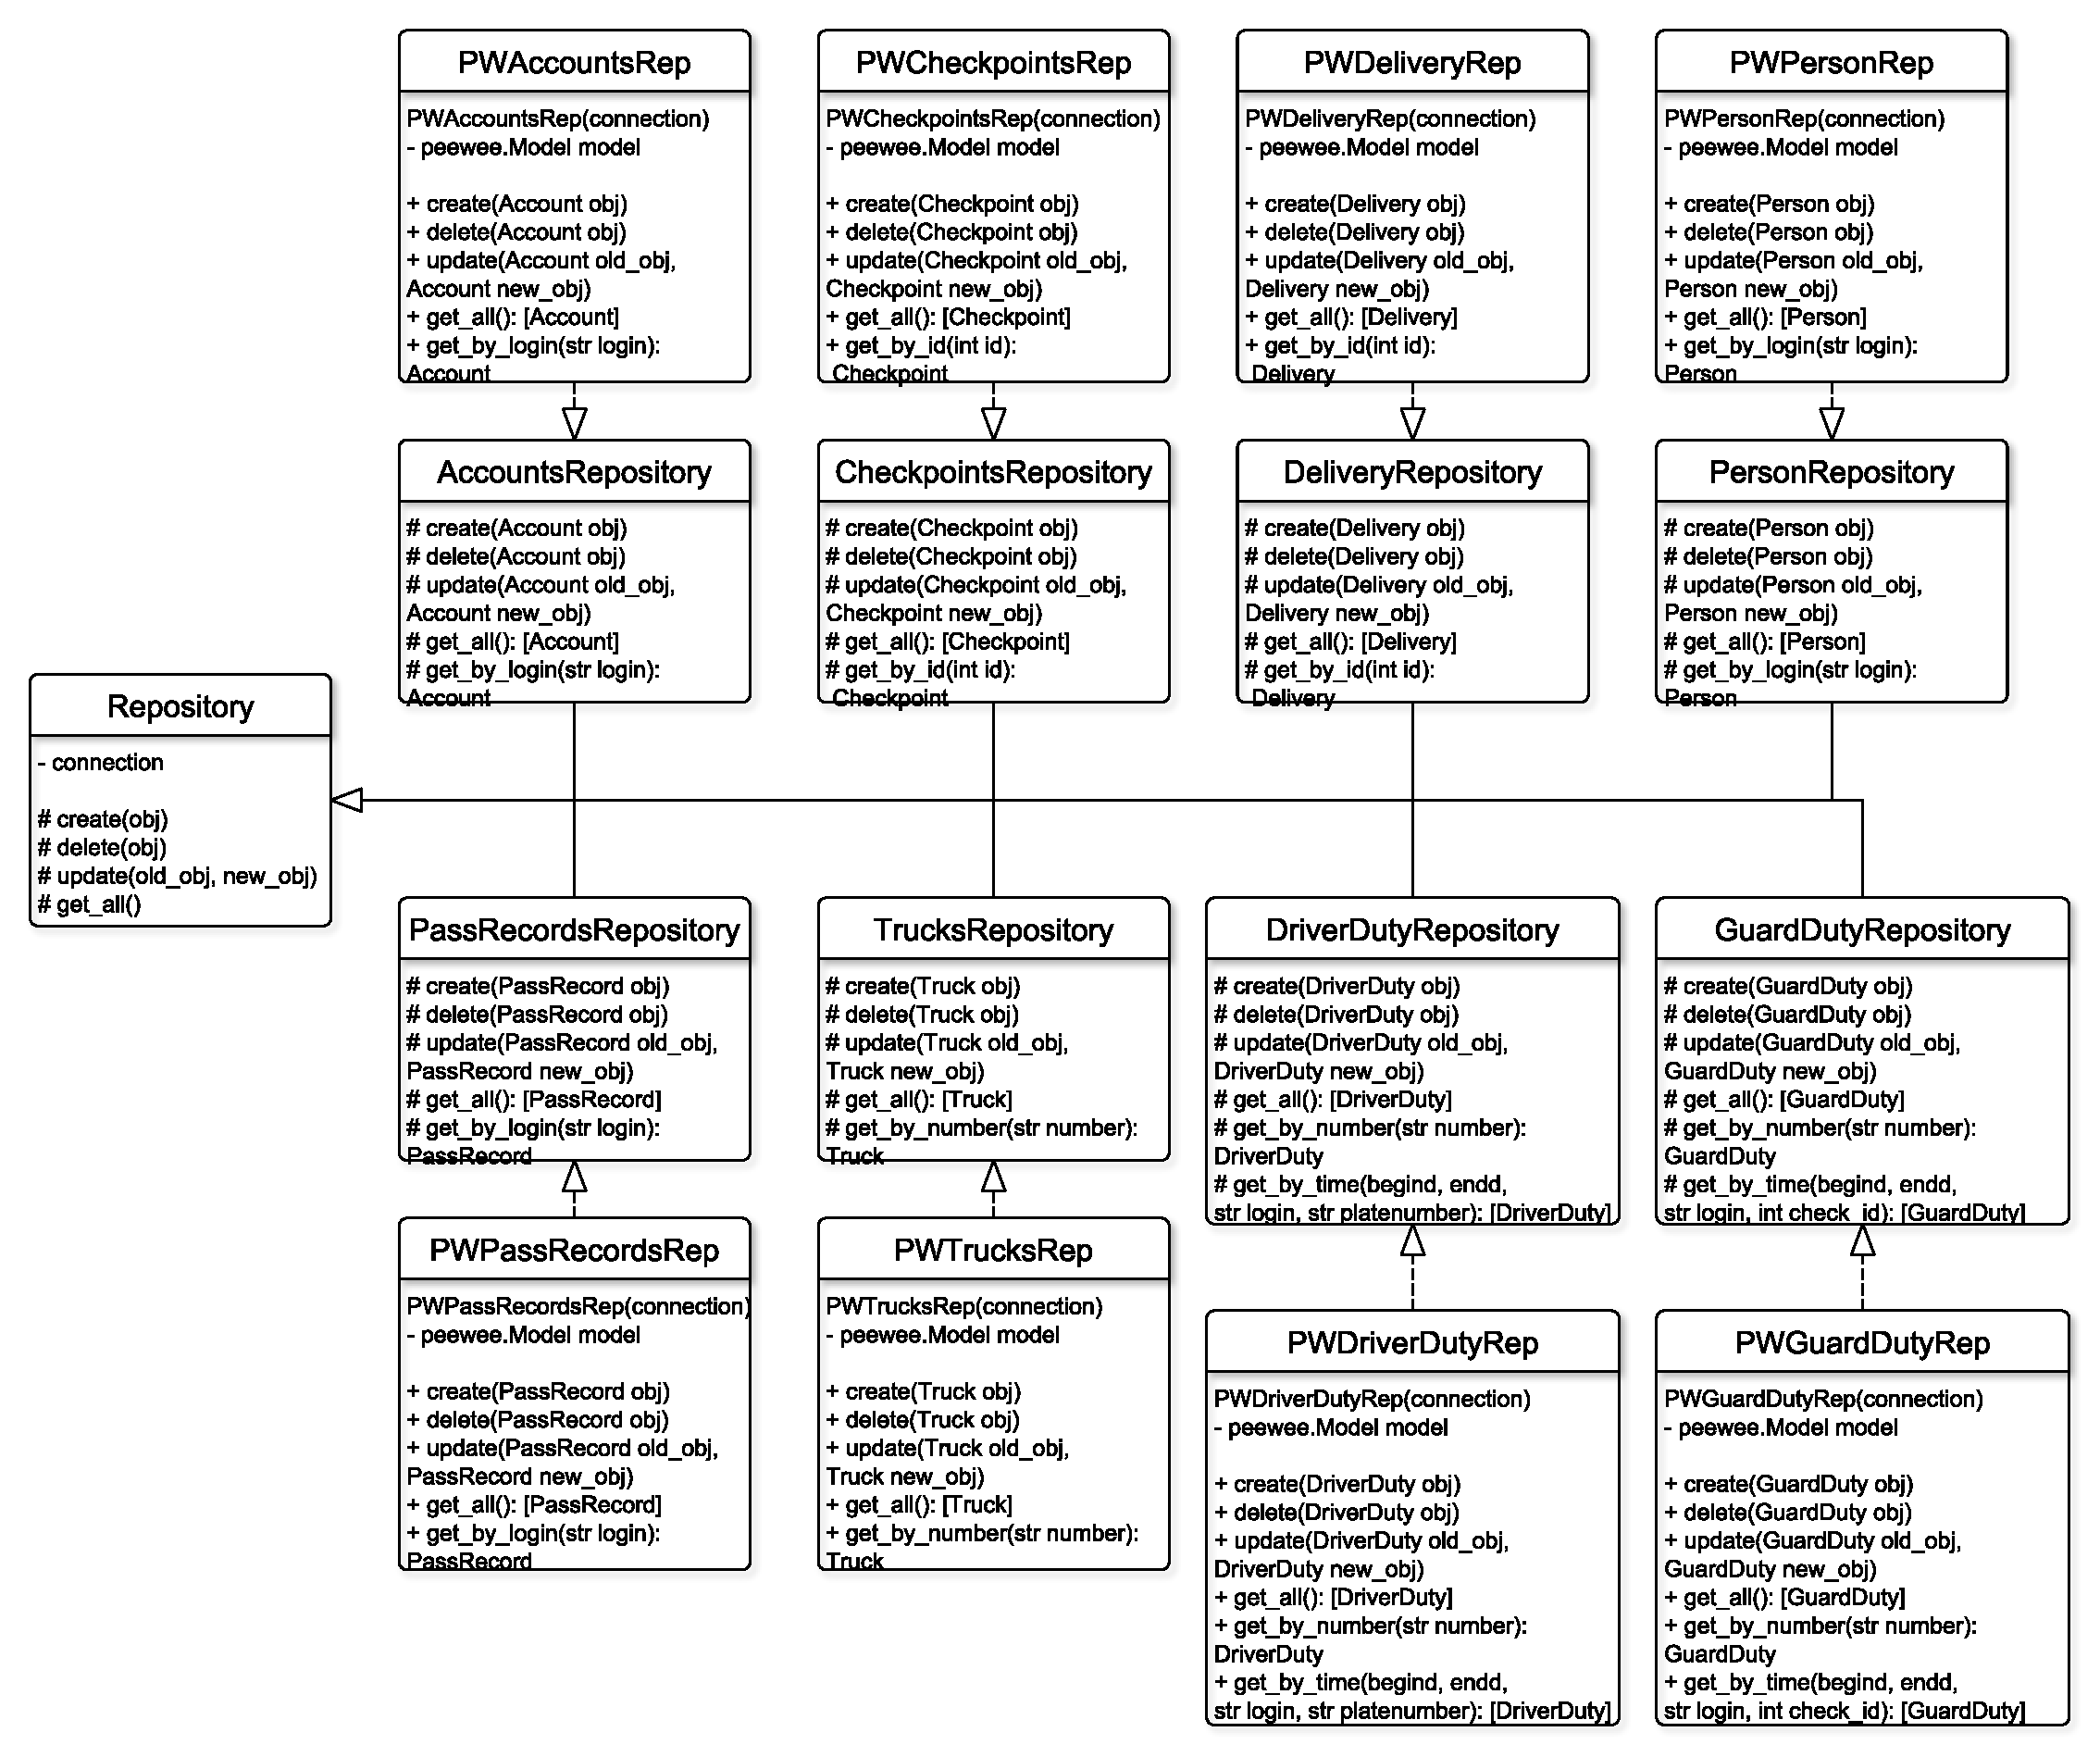
\includegraphics[height=14cm, width = 14cm]{uml/repsoitory.pdf}}
		{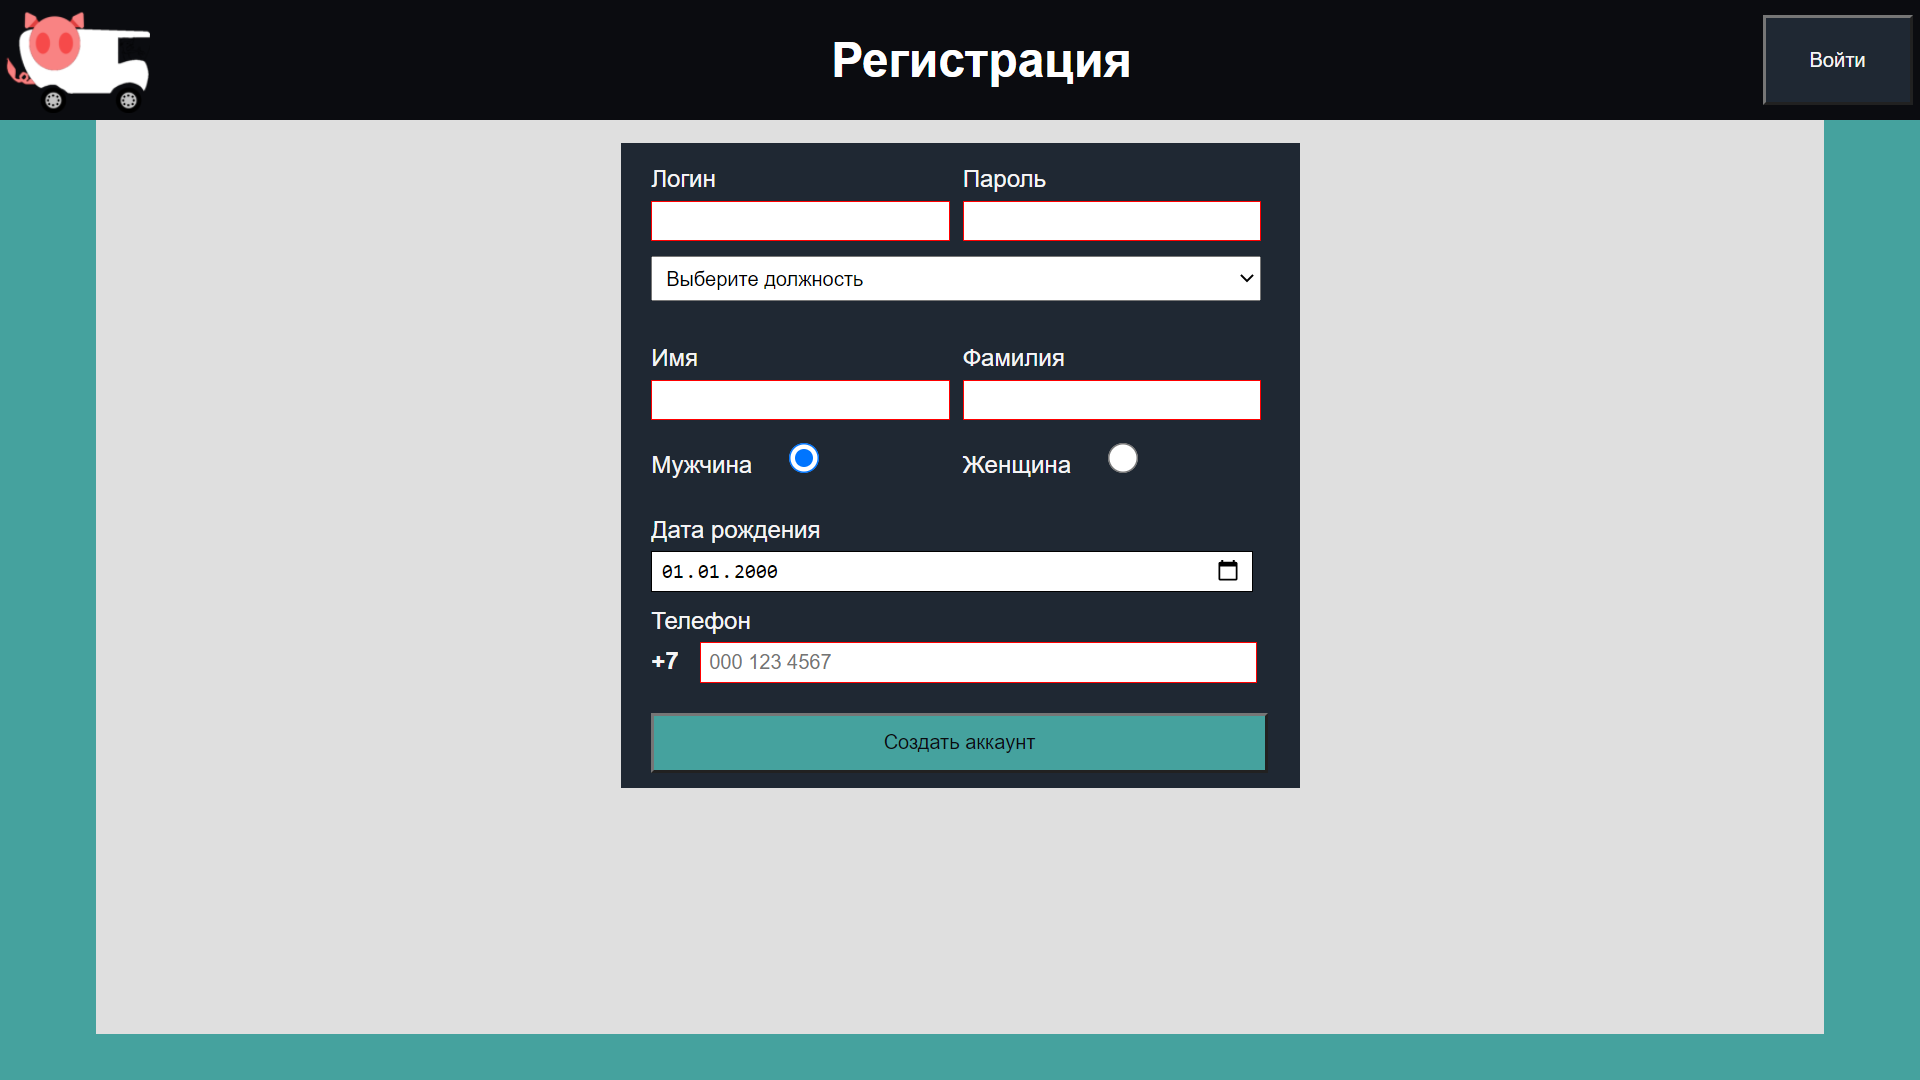
\includegraphics[scale=0.38, angle=0]{sc/signup}}
		\caption{Страница регистрации}
	\end{center}
\end{figure}


\section*{Вывод}
Результатом технологической части стал выбор средств программной реализации, реализация и описание структуры базы данных и приложения, визуальная демонстрация интерфейса приложения.
